%----------------------------------------------------------------------------------------------------------------------
\section{Information Theoretic Analysis}
%----------------------------------------------------------------------------------------------------------------------

As mentioned in Sec.~\ref{sec:sorting-result}, the automated spike sorting had to be abandoned. The dataset used in this section consists of spiking activity manually sorted by the researcher who collected the data.

%----------------------------------------------------------------------------------------------------------------------
\subsection{Methods}

To best illustrate the process gone through in the study, we include some preliminary results amongst the methods.
This is presented so the reader will better understand the decisions taken whilst progressing with the analysis.

%----------------------------------------------------------------------------------------------------------------------
\FloatBarrier
\subsubsection{Artifact elimination}
\label{sec:ma}

Looking at rasters generated to include all the trials across all the sessions, an anomaly was apparent.
For several of the channels in the data from each of the brain regions of each of the animals, some sessions have spikes which align at the same time relative to the stimulus onset. The temporal alignment is very precise, indicating the effect not part of the animal's brain activity but instead due to an external source influencing the detected signal in the recordings. Furthermore, the ``lines'' occurred at regularly spaced intervals, with a period very nearly equal to the refresh rate of the monitor. The spikes across multiple trials line up like this because the experimental equipment will only begin presenting a stimulus when the first pixel on the monitor is being updated, and we of course normalise for the stimulus presentation time across multiple trials.
% INCLUDE RASTER EXAMPLE

An empirical estimate of the artifact periodicity was found by choosing an arbitrary channel which strongly expresses the artifact and measuring by eye the duration of the completed artifact cycles within \unit[530]{ms} (44 for M1, 39 for M2). Since the artifact is tightly localised in time, this could be done with relatively high accuracy. For M1, the period was estimated to be \unit[85.023(1)]{Hz}, whilst for M2 it was \unit[75.023(1)]{Hz}. The discrepancies from the programmed monitor refresh rates of \unit[85]{Hz} and \unit[75]{Hz} respectively can be put down to the specific electronic circuitry used, perhaps issuing the command to the monitor. The discrepancy is small enough to be of little consequence, except we will need \unit[5]{sf} of accuracy rather than \unit[2]{sf} in the following treatment of the artifact. Why it should be out by exactly \unit[0.023]{Hz} for both animals remains unclear, since this corresponds to the refresh cycle running \unit[0.0031]{ms} fast for M1 and \unit[0.0042]{ms} fast for M2. An even bigger mystery is how the artifact has made its way into the recordings. Although it remains possible that the cause is some other piece of equipment also locked to the same refresh cycle, in the following we will refer to this artifact as the ``monitor artifact''. When a collection of datapoints exhibits the monitor artifact, we refer to the data as ``contaminated''.

From the rasters, it seemed as if three-quarters of the channels in M1 V4 were contaminated for at least one session; over two-thirds of the channels for M1 V1 and M2 V4 were contaminated for at least one session; and around a third of the channels for M2 V4 were contaminated for at least one session. The contaminated channels include both high-quality channels with a lot of detected spikes, and low-quality channels with fewer detected spikes. For some of the lowest quality channels and sessions, the artificial spikes were clearly more numerous than the genuine ones. It was considered paramount that the effects of the artifact be corrected for.

To clean up the contamination, a more rigorous method of evaluating the problem was required.
For the collection of spike times from a single channel across multiple trials during a single session, we perform the following steps:
\begin{enumerate}
\item Consider the set of all spiketimes where the visual stimulus has been the same for at least the last \unit[150]{ms}.
\item From each spiketime, $t$, subtract time of nearest stimulus onset/offset, $T_{\text{onset}}$. (Both onset and offset are synchronised with the monitor cycle, and the nearest one offers greatest accuracy.)
$$
t \leftarrow t - T_{\text{onset}}
$$
\item Take the modulo of the spiketimes with respect to the monitor period, $\tau_m$ (\unit[11.7616]{ms} for M1, \unit[13.3292]{ms} for M2).
$$
t \leftarrow t \bmod \tau_m
$$
\item Take a histogram of the spiketimes over bins with the width of the reciprocal of the sampling frequency of the spikes (sampling frequency \unit[32556.000]{Hz}; bin width \unit[0.030716]{ms}).
\end{enumerate}
Conceptually, this is equivalent to stacking all the ``lines'' in the raster on top of each other and seeing how thick the resulting line is.
When the visual stimulus has remained unchanged for at least \unit[150]{ms}, the neurons in V1 and V4 settle down to a steady firing rate, so we expect there to be about the same number of spikes in each of these bins. However, as the monitor artifact increases the number of spikes at set intervals after the monitor refresh commences, there will be an increase in the number of spikes in these bins when the monitor artifact is manifest in the data.

% ./figs/monitor_hist_blanco_v4_ch4_s336_20120817T085037.eps
% ./figs/monitor_hist_jack_v1_ch9_s51_20120817T084845.eps
% ./figs/monitor_hist_jack_v1_ch9_s56_20120817T084855.eps
% ./figs/monitor_hist_jack_v4_ch41_s31_20120817T085111.eps
%%\begin{figure}[htbp]
%%    \begin{subfigure}[b]{0.5\linewidth}
%%        \centering
%%        \caption{}
%%        \label{fig:mahist-b4}
%%        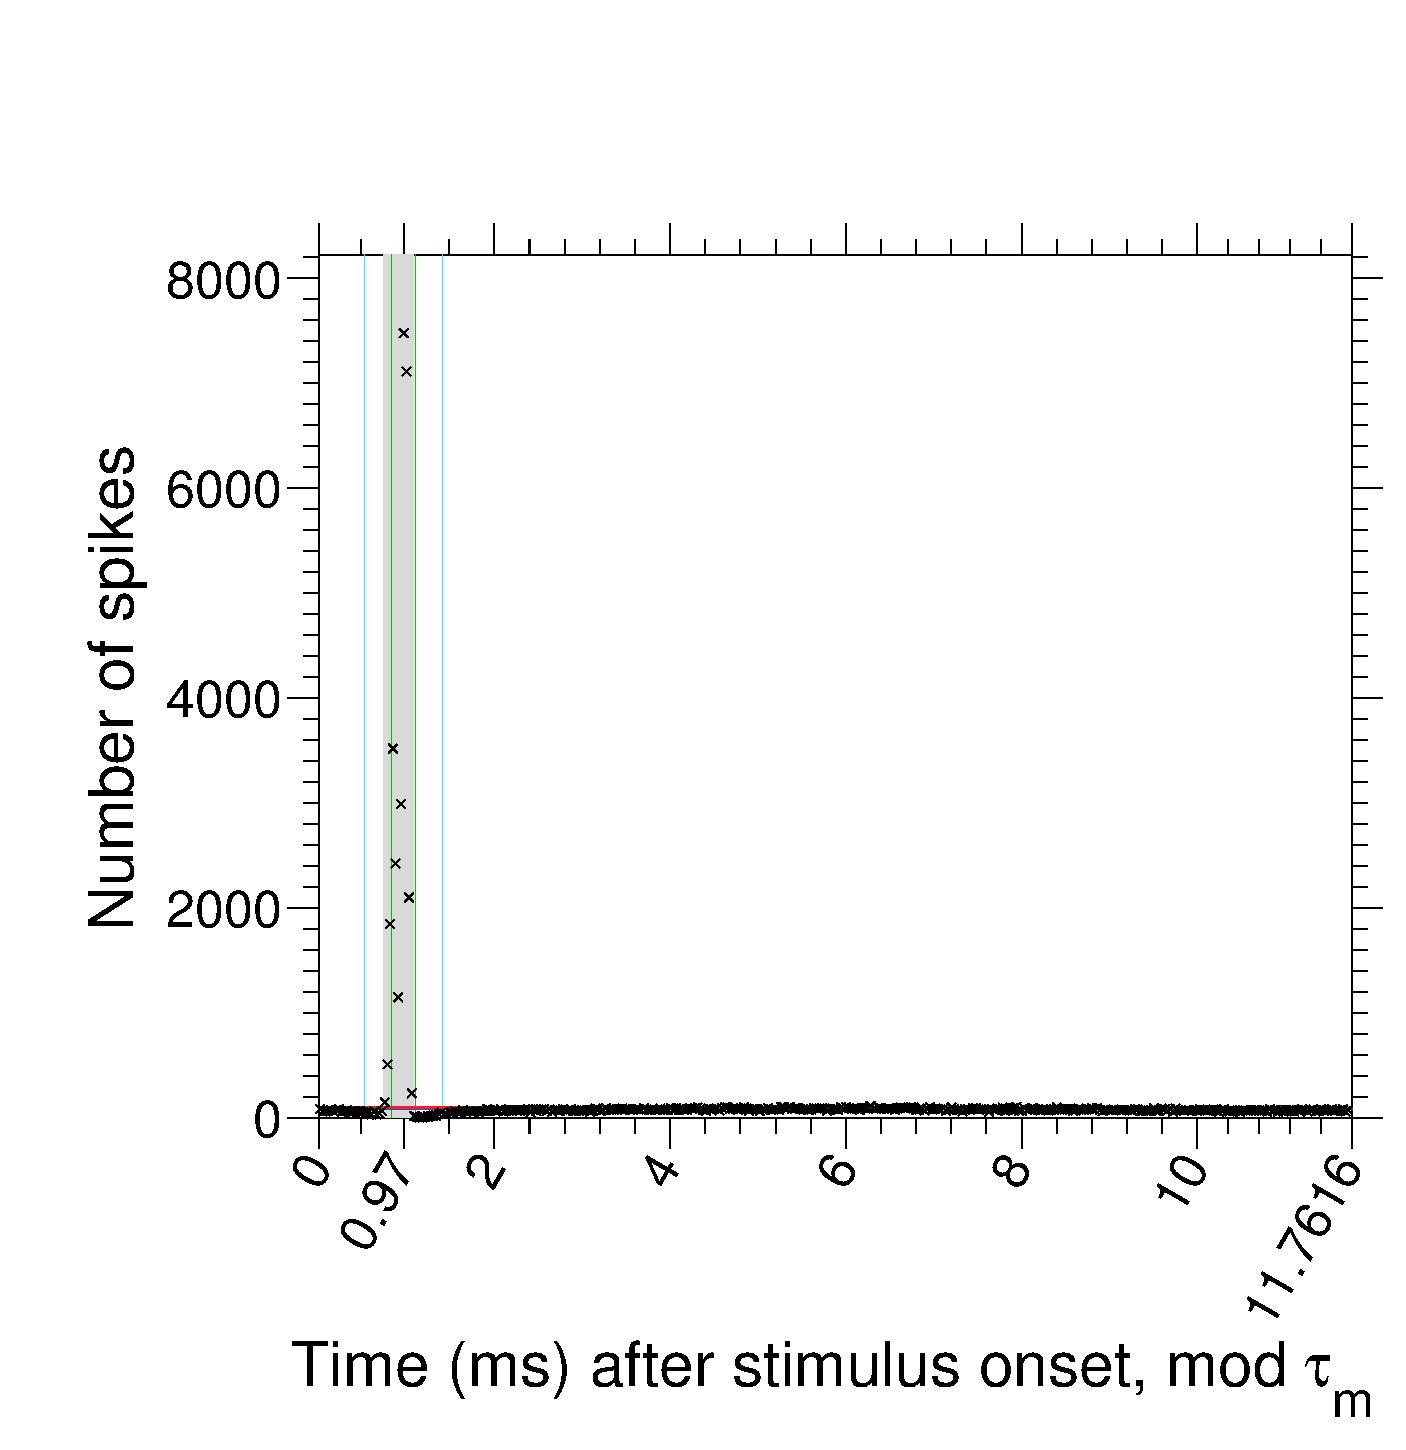
\includegraphics[width=\linewidth]{%
%%./figs/monitor_hist_blanco_v4_ch4_s336_20120817T085037.eps}
%%    \end{subfigure}
%%    ~~
%%    \begin{subfigure}[b]{0.5\linewidth}
%%        \centering
%%        \caption{}
%%        \label{fig:mahist-j4}
%%        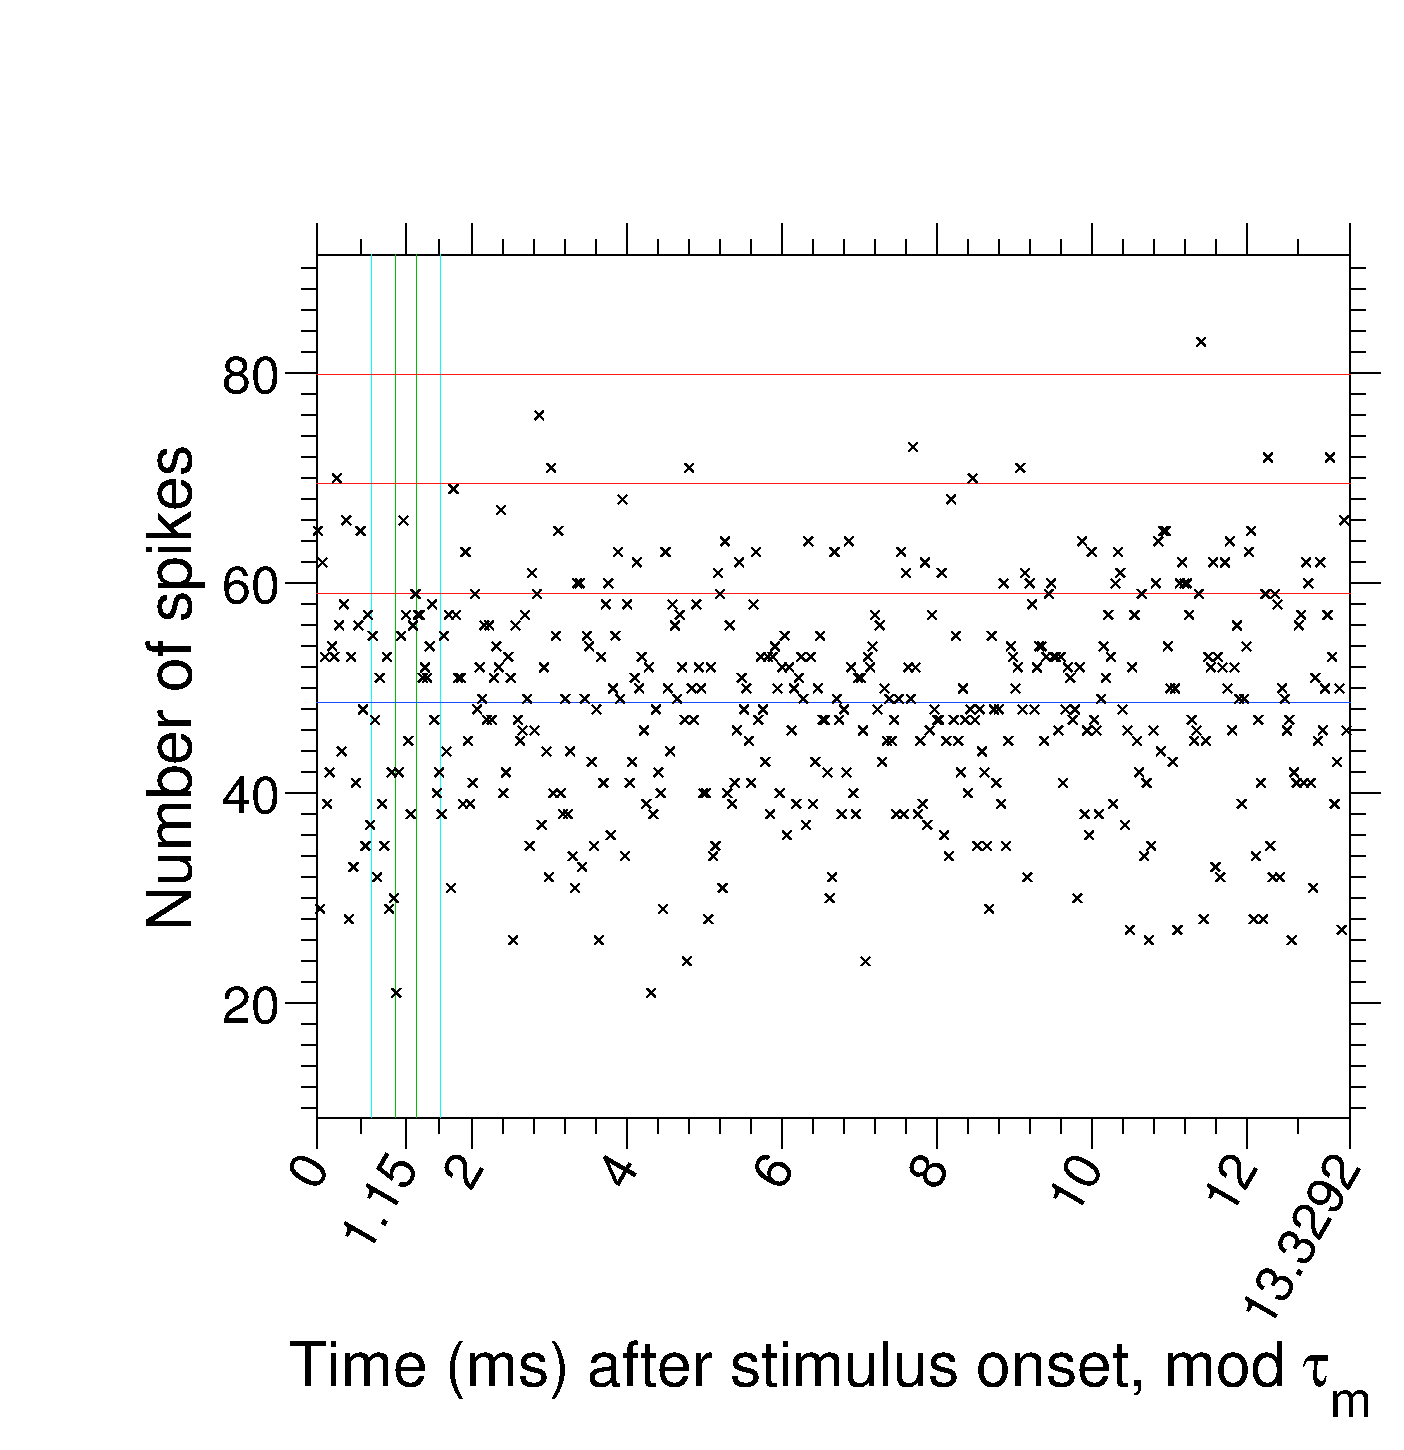
\includegraphics[width=\linewidth]{%
%%./figs/monitor_hist_jack_v4_ch41_s31_20120817T085111.eps}
%%    \end{subfigure}
%%    \\
%%    \begin{subfigure}[b]{0.5\linewidth}
%%        \centering
%%        \caption{}
%%        \label{fig:mahist-j1s51}
%%        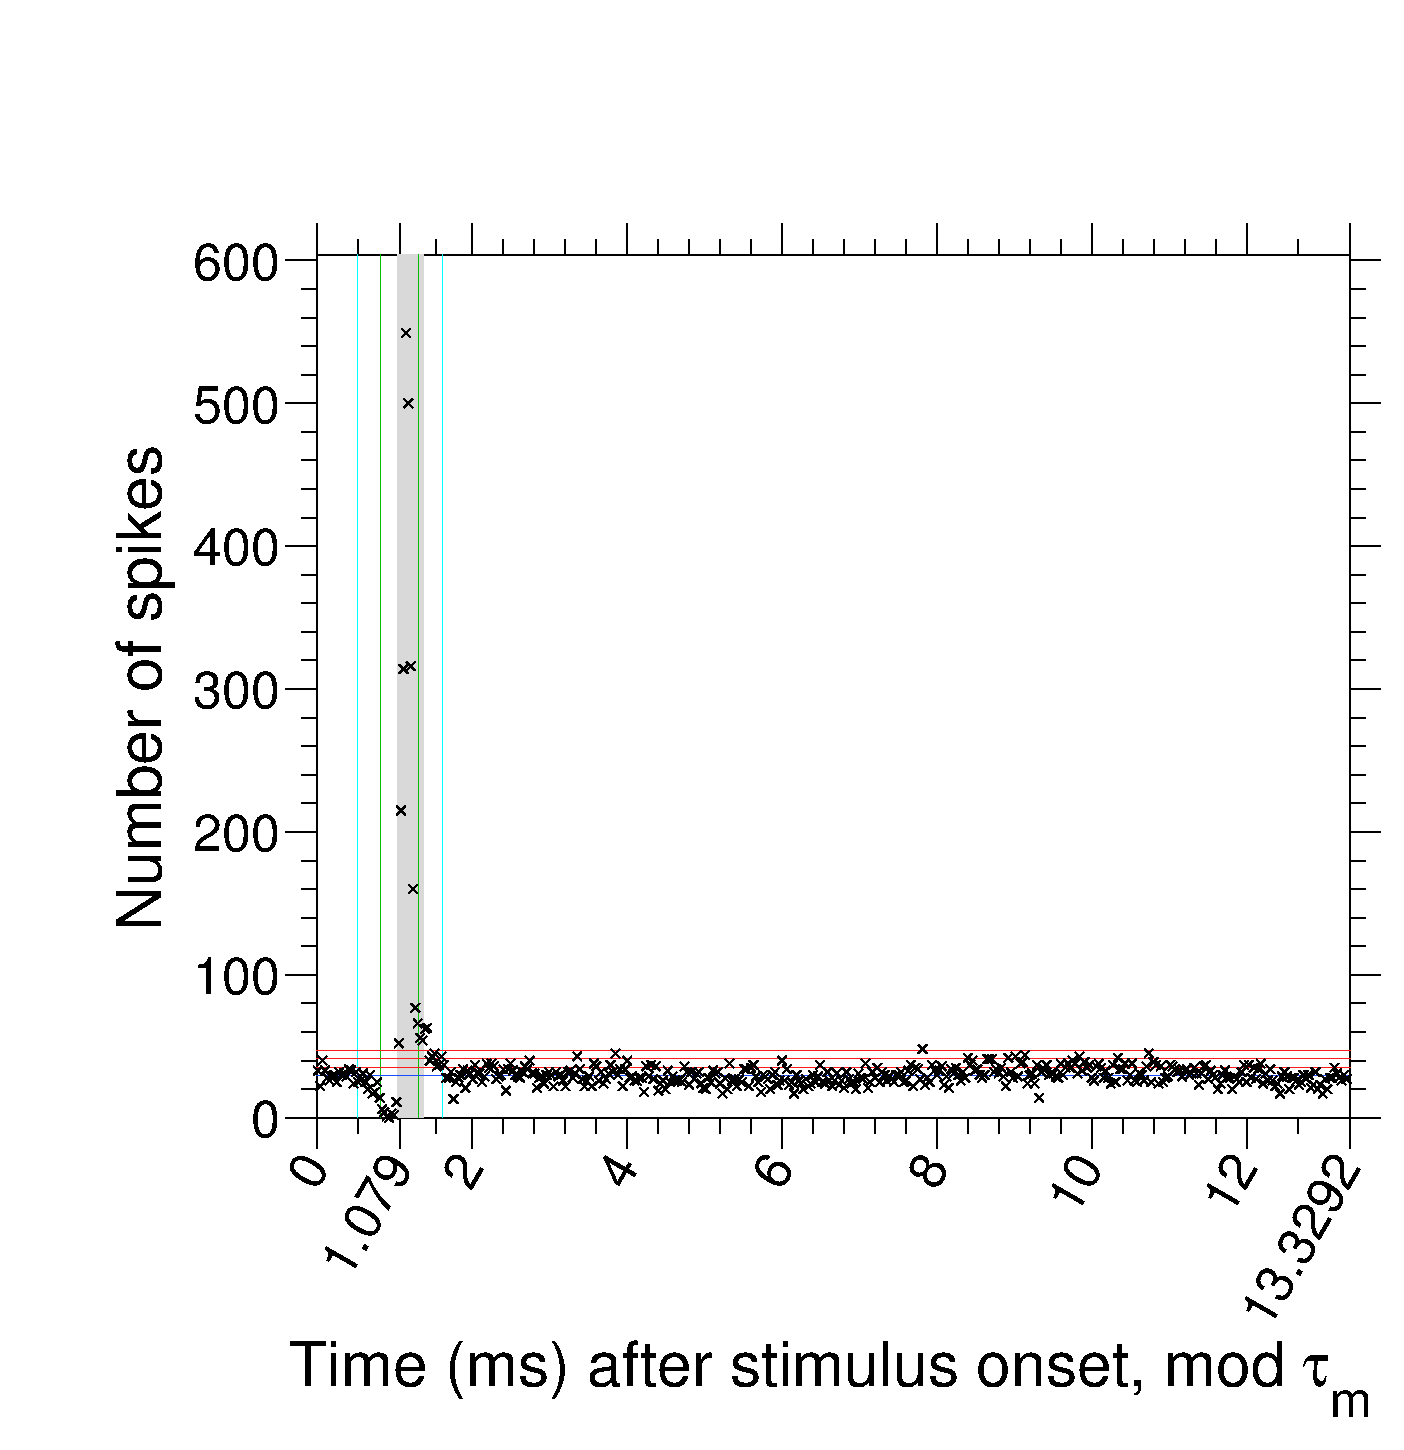
\includegraphics[width=\linewidth]{%
%%./figs/monitor_hist_jack_v1_ch9_s51_20120817T084845.eps}
%%    \end{subfigure}
%%    ~~
%%    \begin{subfigure}[b]{0.5\linewidth}
%%        \centering
%%        \caption{}
%%        \label{fig:mahist-j1s56}
%%        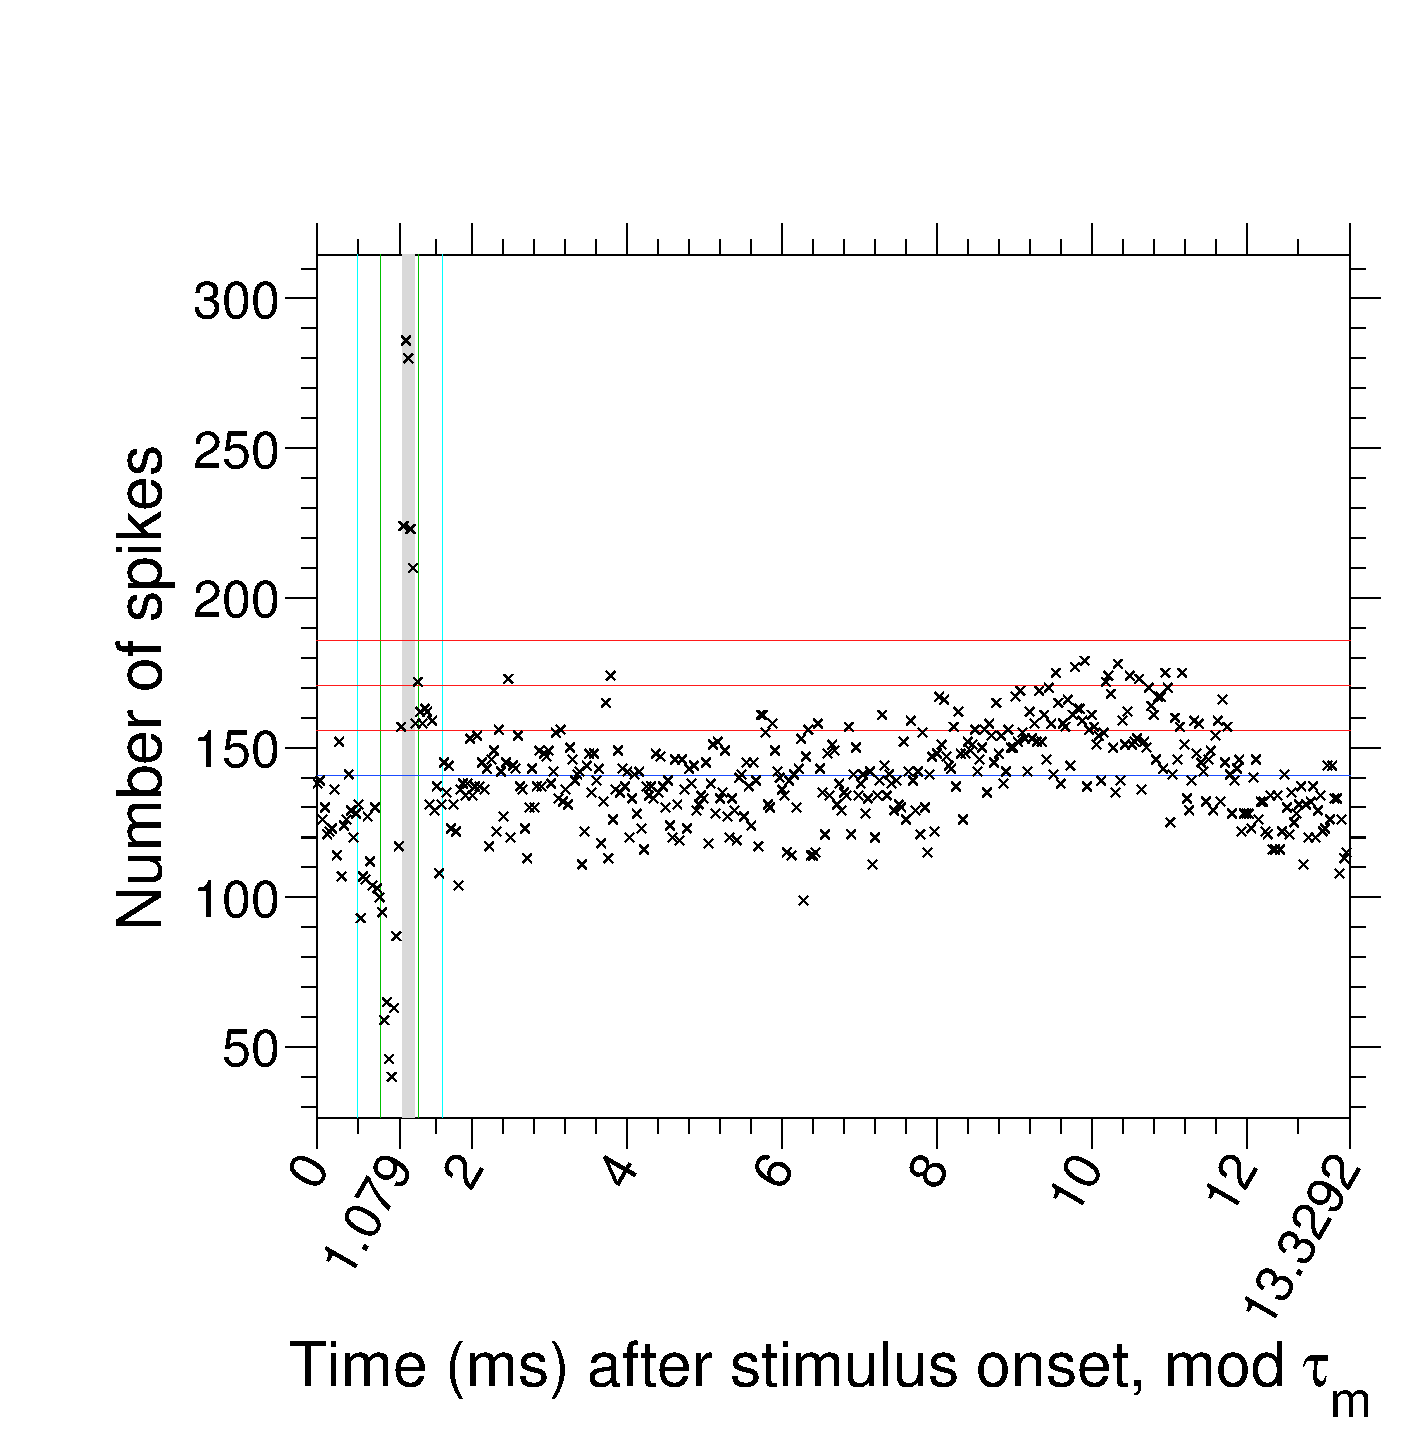
\includegraphics[width=\linewidth]{%
%%./figs/monitor_hist_jack_v1_ch9_s56_20120817T084855.eps}
%%    \end{subfigure}
%%    \caption{Crosses: Histogram of spikes in bins of width \unit[0.030716]{ms}.
%%\ref{fig:mahist-b4}: M1 V4, channel 4, session 336; a channel and session very strongly exhibiting the monitor artifact.
%%\ref{fig:mahist-j4}: M2 V4, channel 41, session 31; a dataset where the artifact is not present.
%%\ref{fig:mahist-j1s51}: M2 V1, channel 9, session 51; data strongly presenting the monitor artifact.
%%\ref{fig:mahist-j1s56}: M2 V1, channel 9, session 56; data mildly showing the effect of the monitor artifact.
%%Green vertical lines: extremities of search window (contained between the lines).
%%Cyan vertical lines: extremities of mean region.
%%Blue line: mean of the data (excluding area between cyan lines).
%%Red lines: mean plus 1, 2 and 3 standard deviations respectively.
%%Gray background: Spikes marked as contaminated and scheduled for redaction.
%%}
%%    \label{fig:mahist}
%%\end{figure}

% INSERT HIST FIGURE 

As shown in Fig.~\ref{fig:mahist}, the analysis conforms to our expectations.
However, doing the analysis in this more rigorous manner revealed the contamination was more widespread than previously assumed. The histograms of spiketimes indicate that more sessions are contaminated than not, and only a couple of channels are completely clean for every session.

For the most part, the timing of the monitor artifact $\bmod \tau_m$ is very reliable and it affects the same 6 or so bins whenever the data is contaminated. The contaminated part of each monitor cycle is thus restricted to at most \unit[0.2]{ms}, and, assuming this period of time contains both genuine spikes and artificial spikes, if we simply delete all datapoints with this \unit[0.2]{ms} window, we will lose at most less than 2\% of the genuine spikes. This level of data loss is not terribly significant, and justifiable for the gain in reliability of the remaining dataset, particularly for sessions where artificial spikes seem to be more common than genuine ones.

\begin{table}[hbtp]
\caption{Typical time of the peak in number of spikes due to the monitor artifact effect. The time is given relative to the start of the monitor refresh as given by the stimulus onset times. Monitor artifacts occur at $t = t^*_m + k \tau_m$, for $k \in \Z$. For channels recording from M2 V1, the artifact will occur at one of the two stated times throughout a given session, but which of the two varies from channel-to-channel for any individual session, and from session-to-session for any individual channel. Why this happens is unclear.}
\label{tab:mapeak}
\begin{center}
\begin{tabular}{rlc}
\toprule
Animal  & Region & Time of artifact peak $t^*_m$ $\pm 0.01$ (\unit{ms})
\\
\midrule
M1  & V1    & 0.95
\\
        & V4    & 0.97
\\
M2    & V1    & either 0.97 or 1.19
\\
        & V4    & 1.15
\\
\bottomrule
\end{tabular}
\end{center}
\end{table}

% However it is apparent that this method is not great (see jack v1 ch7 s57)

However, it is possible to do better that this and to isolate and remove only the contaminated bins. As shown in Fig.~\ref{fig:mahist}, the effect of the artifact is greater for some sessions than others and
From observations on the typical width time of the width and peak time (Table.~\ref{tab:mapeak}) of the artifact, along with its periodicity ($\tau_m$), the following method of removal was devised and implemented.
\begin{enumerate}
\item Perform the modulo $\tau_m$ and take the histogram as described above.
\item Define the ``search region'' as bins which contain spike within $t^*_m \pm \unit[0.130]{ms}$, so we have one bin more than the anticipated artifact width in either direction. (For M2 V1, we use the range \unit[$(0.968 - 0.130 , 1.190 + 0.130)$]{ms}.)
\item Find the mean, $\mu$, and standard deviation, $\sigma$, of all the bins which are at least 10 away (\unit[0.3]{ms} away) from the search region. We also exclude the final bin since $0.030716 \bmod \tau_m \neq 0$ and it is only part-full.
\item If any one of the bins in the search region exceeds $\mu + 3 \sigma$, we declare the session contaminated and proceed with the following steps. If not, it is declared intact and left as it is.
\item All bins in the search region which contain more than $\mu + 3 \sigma$ spikes are declared contaminated.
\item Let $t_m$ denote the time of the centre of the bin in the search region containing the most spikes.
\item All bins which contain spikes within $t_m \pm \unit[0.1]{ms}$ are placed in ``quarantine''.
\item All quarantined bins which contain more than $\mu + 2.5 \sigma$ spikes are declared contaminated.
\item All bins between the first and last contaminated bins are declared contaminated.
\item Consider immediate neighbours of the first bin and if they are also contain more than $\mu + 2.5 \sigma$ spikes, they are declared contaminated.
\item Repeat the above step until either a neighbour is found which is not contaminated, or until a maximum of three bins have been added to the contaminated region.
\item Consider immediate neighbours of the last bin and if they are also contain more than $\mu + 2.5 \sigma$ spikes, they are declared contaminated.
\item Repeat the above step until either a neighbour is found which is not contaminated, or until a maximum of three bins have been added to the contaminated region.
\item Consider the full dataset of spikes for this particular channel and session.
\item For each spike, consider which bin its spiketime would be arranged into.
\item If it is a contaminated bin, the spike is removed from the dataset.
\end{enumerate}

This allows us to have prior assumptions about the location and width of the monitor artifact effect, but be flexible about exactly where it falls and which sets of bins are affected.
It is possible that the dynamically targeted removal method may cause issues due to inconsistency in the data across different sessions, but there is a clearly a gain in the amount of preserved data and a gain in the reliability of the data which remains.

%----------------------------------------------------------------------------------------------------------------------
\FloatBarrier
\subsubsection{Session-based analysis}

merged all neurons together for a single channels

Neurolynx NSE files were loaded into MATLAB using the Neurolynx supplied code when operating on Windows, and an version 6 of an unofficial port for Linux (recommended by Neurolynx) otherwise.%
\footnote{Available at
\\ \url{http://www.urut.ch/new/serendipity/index.php?/pages/downloads.html}}

The information was computed for each day of training (hereafter referred to as a session), for each of the channels from which recordings were available. To gauge the typical behaviour of a neuron, the mean was taken over all the channels.
The mutual information between the spiking activity during test presentation and the identity of the test stimulus was computed
using a spike-timing based code.
This computation was done using the \verb|information| function from the freely available Information Break-down Toolbox \cite{Magri2009} for MATLAB.%
\footnote{Available at \url{http://www.ibtb.org}}

A moving window of $\unit[20]{ms}$ was taken and subdivided into 5 sequential bins, each of $\unit[4]{ms}$.
The number of spikes within each of the 5 bins was totalled up to provide a code letter for the bin.
The combination of the 5 sequential counts forms a codeword.

This is performed across all the trials in a session with the $\unit[20]{ms}$ window placed with the same offset relative to the test stimulus onset.
By assembling the trials according to their test contrast, the mutual information between the contrast and the spiking activity in this window can be computed.

Following the methods employed by the research group, only trials in which the monkey responded correctly were used for this analysis.

%----------------------------------------------------------------------------------------------------------------------
% 5bins of 4ms
% ./figs/I_sessionwise_blanco_v1_chmean23_s343-359_oc1_5bins_of_4ms_dr_naive_pcolorhot_20120815T150057.png
% ./figs/I_sessionwise_blanco_v4_chmean31_s307,308,311,313,314,317,318,320,321,329-341_oc1_5bins_of_4ms_dr_naive_pcolorhot_20120815T150100.png
% ./figs/I_sessionwise_jack_v1_chmean25_s51-72_oc1_5bins_of_4ms_dr_naive_pcolorhot_20120815T150049.png
% ./figs/I_sessionwise_jack_v4_chmean20_s24-49_oc1_5bins_of_4ms_dr_naive_pcolorhot_20120815T150053.png
% 1 bin of 20ms
% ./figs/I_sessionwise_blanco_v1_chmean23_s343-359_oc1_1bins_of_20ms_dr_naive_pcolorhot_20120815T190833.png
% ./figs/I_sessionwise_blanco_v4_chmean31_s307,308,311,313,314,317,318,320,321,329-341_oc1_1bins_of_20ms_dr_naive_pcolorhot_20120815T190836.png
% ./figs/I_sessionwise_jack_v1_chmean25_s51-72_oc1_1bins_of_20ms_dr_naive_pcolorhot_20120815T190825.png
% ./figs/I_sessionwise_jack_v4_chmean20_s24-49_oc1_1bins_of_20ms_dr_naive_pcolorhot_20120815T190829.png
% 
% ./figs/I_sessionwise_blanco_v1_chmean23_s343-359_oc1_5bins_of_4ms_dr_naive_pcolorhot_20120815T202102.png
% ./figs/I_sessionwise_blanco_v4_chmean31_s307,308,311,313,314,317,318,320,321,329-341_oc1_5bins_of_4ms_dr_naive_pcolorhot_20120815T202106.png
% ./figs/I_sessionwise_jack_v1_chmean25_s51-72_oc1_5bins_of_4ms_dr_naive_pcolorhot_20120815T202053.png
% ./figs/I_sessionwise_jack_v4_chmean20_s24-49_oc1_5bins_of_4ms_dr_naive_pcolorhot_20120815T202058.png


%%\begin{figure}
%%\centering
%%\subfloat[A big tikz picture.\label{fig:one}]{%
%%  \makebox[\textwidth][l]{% %%% as above
%%  \resizebox{.45\largefigure}{!}{%
%%    \input{fig/tikzfile}}}}%
%%\hfill%
%%\subfloat[Another big tikz picture.\label{fig:two}]{%
%%  \makebox[\textwidth][l]{% %%% as above
%%  \resizebox{.45\largefigure}{!}{%
%%    \input{fig/tikzfile}}}}%
%%\caption{Two tikz pictures}
%%\label{fig:label}
%%\end{figure}
%%
%%\begin{figure}%
%%\centering
%%\subfloat[][]{...figure code...}%
%%\qquad
%%\subfloat[][]{...figure code...}%
%%\caption{Here are the first two figures of a continued figure.}%
%%\label{fig:cont}%
%%\end{figure}

\begin{figure}[htbp]%
    \centering
    \subfloat[][M1 V1.\label{fig:sessb1}]{%
        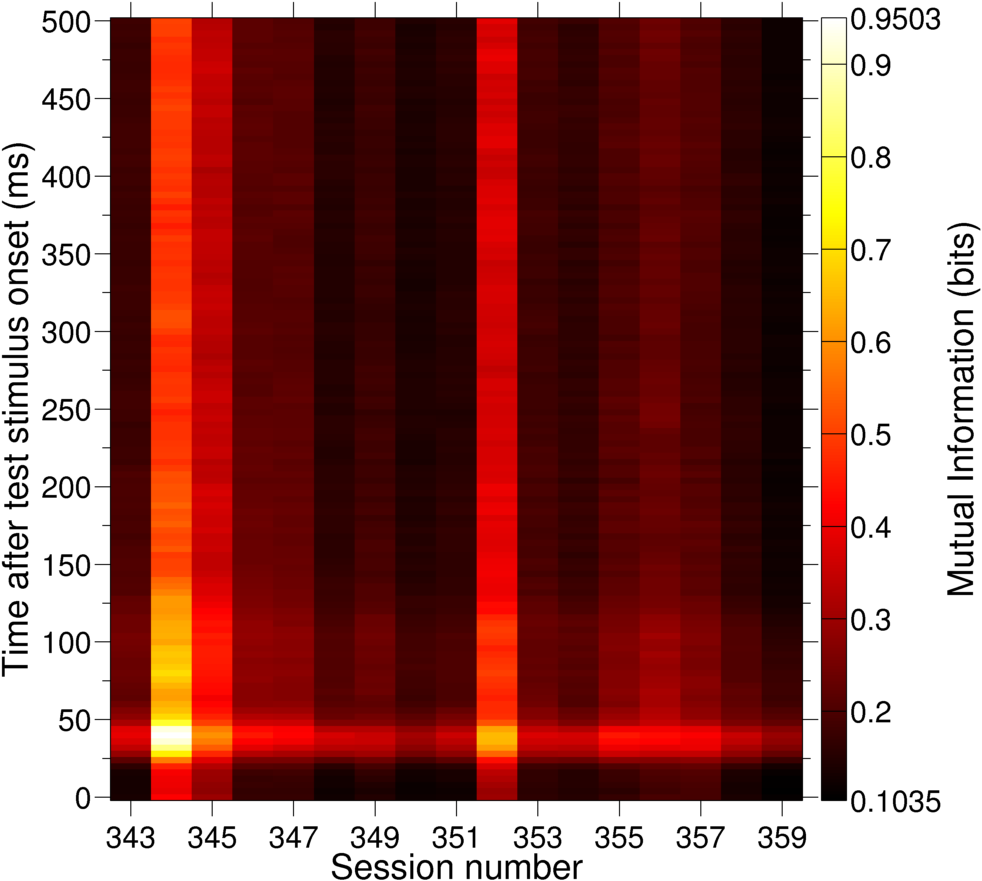
\includegraphics[scale=.25]{%
./figs/I_sessionwise_blanco_v1_chmean23_s343-359_oc1_5bins_of_4ms_dr_naive_pcolorhot_20120815T202102.png}
    }%
    ~~
    \subfloat[][M1 V4.\label{fig:sessb4}]{%
        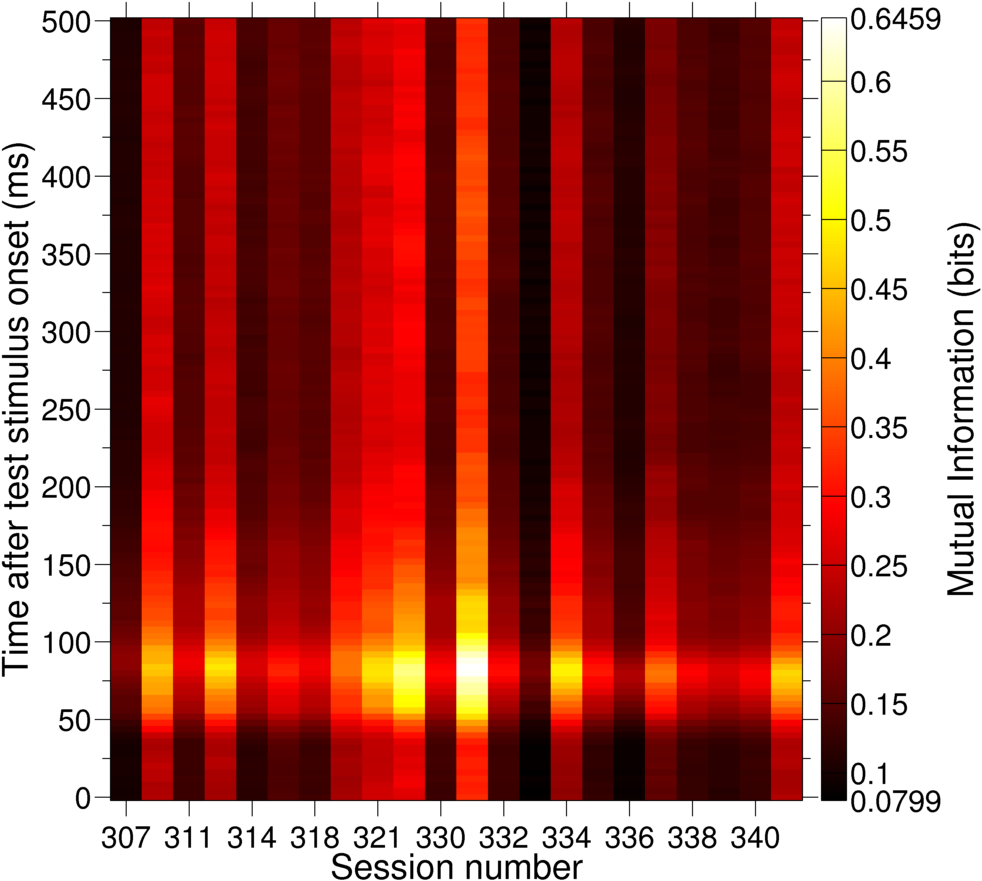
\includegraphics[scale=.25]{%
./figs/I_sessionwise_blanco_v4_chmean31_s307,308,311,313,314,317,318,320,321,329-341_oc1_5bins_of_4ms_dr_naive_pcolorhot_20120815T202106.png}
    }%
    \\
    \subfloat[][M2 V1.\label{fig:sessj1}]{%
        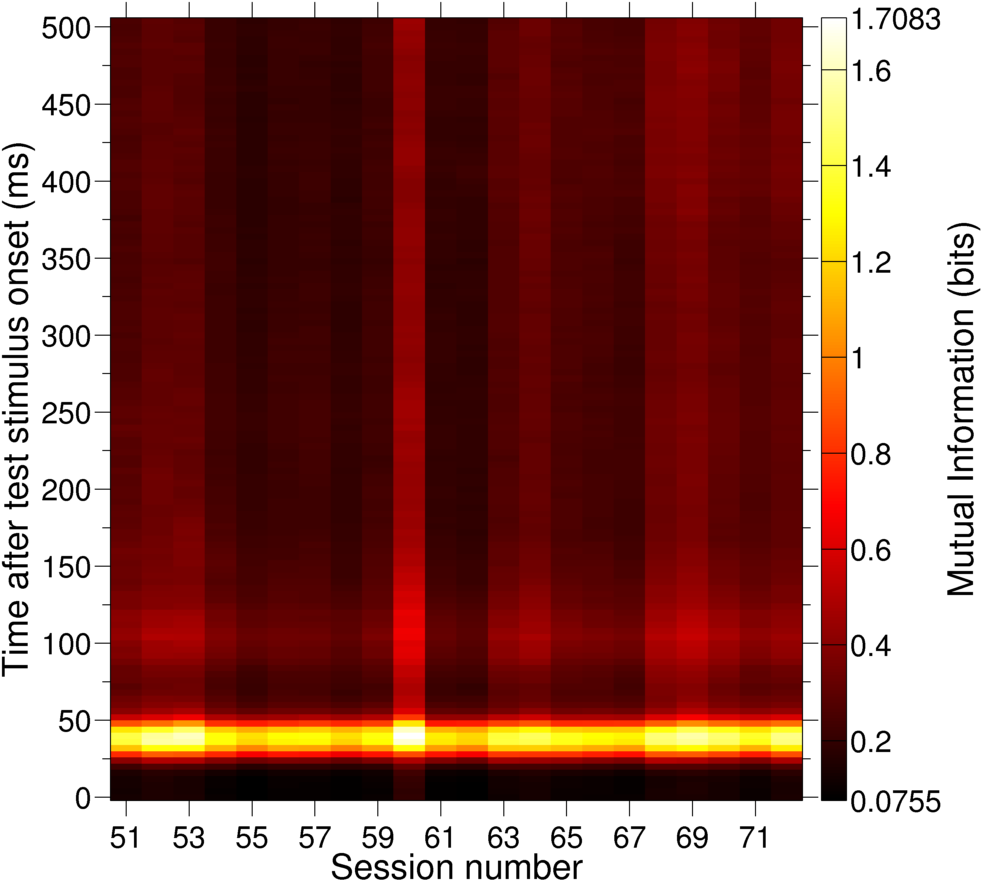
\includegraphics[scale=.25]{%
./figs/I_sessionwise_jack_v1_chmean25_s51-72_oc1_5bins_of_4ms_dr_naive_pcolorhot_20120815T202053.png}
    }%
    ~~
    \subfloat[][M2 V4.\label{fig:sessj4}]{%
        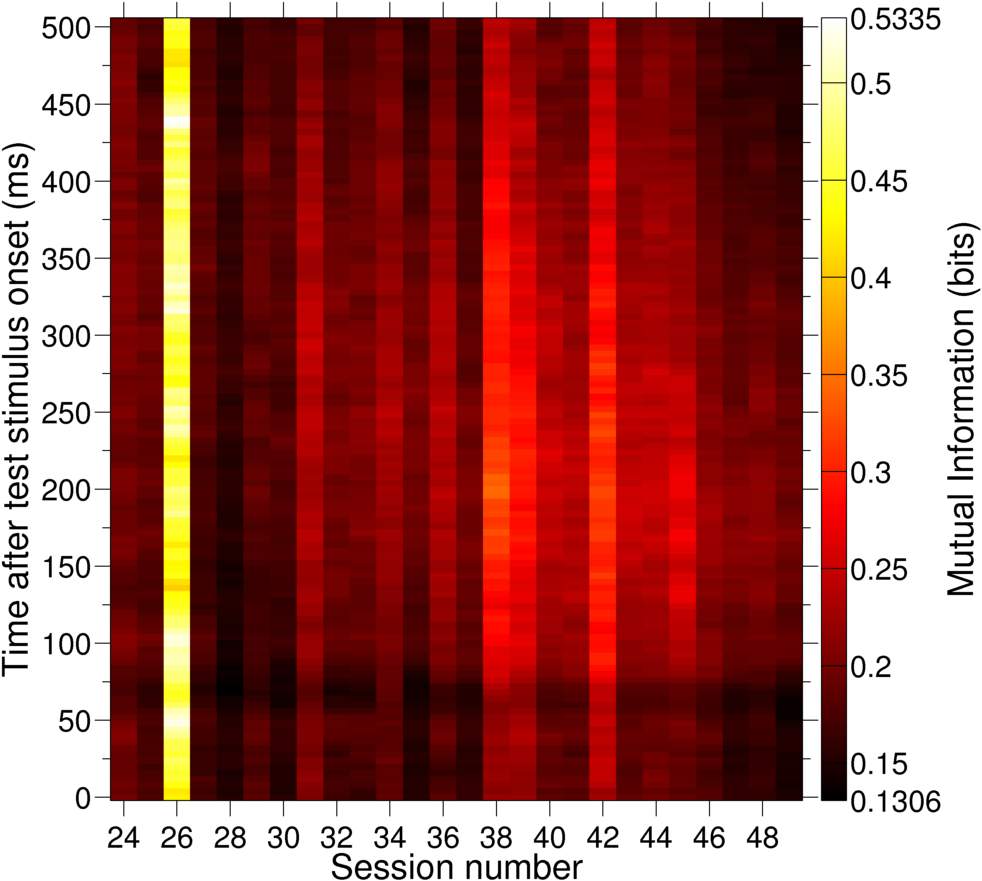
\includegraphics[scale=.25]{%
./figs/I_sessionwise_jack_v4_chmean20_s24-49_oc1_5bins_of_4ms_dr_naive_pcolorhot_20120815T202058.png}
    }%
    \caption{Mutual information between the test stimulus and the neural activity during test presentation.
The mutual information with the test stimulus is taken for a spike timing based code for a \unit[20]{ms} window of spiking activity, sampled with the start of the window offset ($y$-axis) from \unit[0]{ms} up to \unit[500]{ms} after test stimulus onset (which is slightly more than \unit[20]{ms} before test stimulus offset). The sampling is in intervals of \unit[5]{ms}, so any 4 adjacent squares within each session are highly correlated.
The recording session number for the data is given along the $x$-axis, and the number of days the animal has been trained for increases from left to right.
Average mutual information across all the channels is denoted by the pseudo-colour of each of the rectangular patches, centred around the $(x,y)$ co-ordinate to which the measurement relates.
In each case the average is taken across all available channel data: \ref{fig:sessb1}~23 channels, \ref{fig:sessb4}~30 channels, \ref{fig:sessj1}~25 channels, \ref{fig:sessj4}~20 channels.
% The PT bias correction method was used (see text).
The plug-in method without bias correction was used (see text).
}
    \label{fig:sess}
\end{figure}

% ./figs/I_sessionwise_blanco_v1_chmean23_s343-359_oc1_5bins_of_4ms_dr_pt_pcolorhot_20120811T130028.eps
% ./figs/I_sessionwise_blanco_v4_chmean31_s307,308,311,313,314,317,318,320,321,329-341_oc1_5bins_of_4ms_dr_pt_pcolorhot_20120811T130522.eps
% ./figs/I_sessionwise_jack_v1_chmean25_s51-72_oc1_5bins_of_4ms_dr_pt_pcolorhot_20120811T130003.eps
% ./figs/I_sessionwise_jack_v4_chmean20_s24-49_oc1_5bins_of_4ms_dr_pt_pcolorhot_20120811T133212.eps

The results of this initial analysis are shown in Fig.~\ref{fig:sess}.
% Although the relationship between different window offsets and the mutual information is similar for each of the sessions, the
No trend in information content with learning can be discerned because the measured mutual information content varies wildly from session-to-session.

% %----------------------------------------------------------------------------------------------------------------------
% \chapter{}
% %----------------------------------------------------------------------------------------------------------------------
% \subsection{Methods}


% Demonstrate how this is dominated by the number of trials in the session, regardless of bias correction technique

% ./figs/ntrialsIbyNindiv_blanco_v1_dr_naive_20120812T164553.eps
% ./figs/ntrialsIbyNindiv_blanco_v4_dr_naive_20120812T164553.eps
% ./figs/ntrialsIbyNindiv_jack_v1_dr_naive_20120812T164553.eps
% ./figs/ntrialsIbyNindiv_jack_v4_dr_naive_20120812T164553.eps
%
% ./figs/ntrialsIandNindiv_blanco_v1_dr_naive_20120812T175154.eps
% ./figs/ntrialsIandNindiv_blanco_v4_dr_naive_20120812T175154.eps
% ./figs/ntrialsIandNindiv_jack_v1_dr_naive_20120812T175154.eps
% ./figs/ntrialsIandNindiv_jack_v4_dr_naive_20120812T175154.eps
%
% ./figs/ntrialsIandNindiv_blanco_v1_dr_naive_1bins_of_20ms_20120815T200333.eps
% ./figs/ntrialsIandNindiv_blanco_v4_dr_naive_1bins_of_20ms_20120815T200333.eps
% ./figs/ntrialsIandNindiv_jack_v1_dr_naive_1bins_of_20ms_20120815T200333.eps
% ./figs/ntrialsIandNindiv_jack_v4_dr_naive_1bins_of_20ms_20120815T200333.eps
% 
% ./figs/ntrialsIandNindiv_blanco_v1_dr_naive_5bins_of_4ms_20120815T201856.eps
% ./figs/ntrialsIandNindiv_blanco_v4_dr_naive_5bins_of_4ms_20120815T201856.eps
% ./figs/ntrialsIandNindiv_jack_v1_dr_naive_5bins_of_4ms_20120815T201856.eps
% ./figs/ntrialsIandNindiv_jack_v4_dr_naive_5bins_of_4ms_20120815T201856.eps
% 
% % \begin{figure}[htbp]
% %     \begin{subfigure}[b]{0.5\linewidth}
% %         \centering
% %         \caption{M1 V1}
% %         \label{fig:IandNb1}
% %         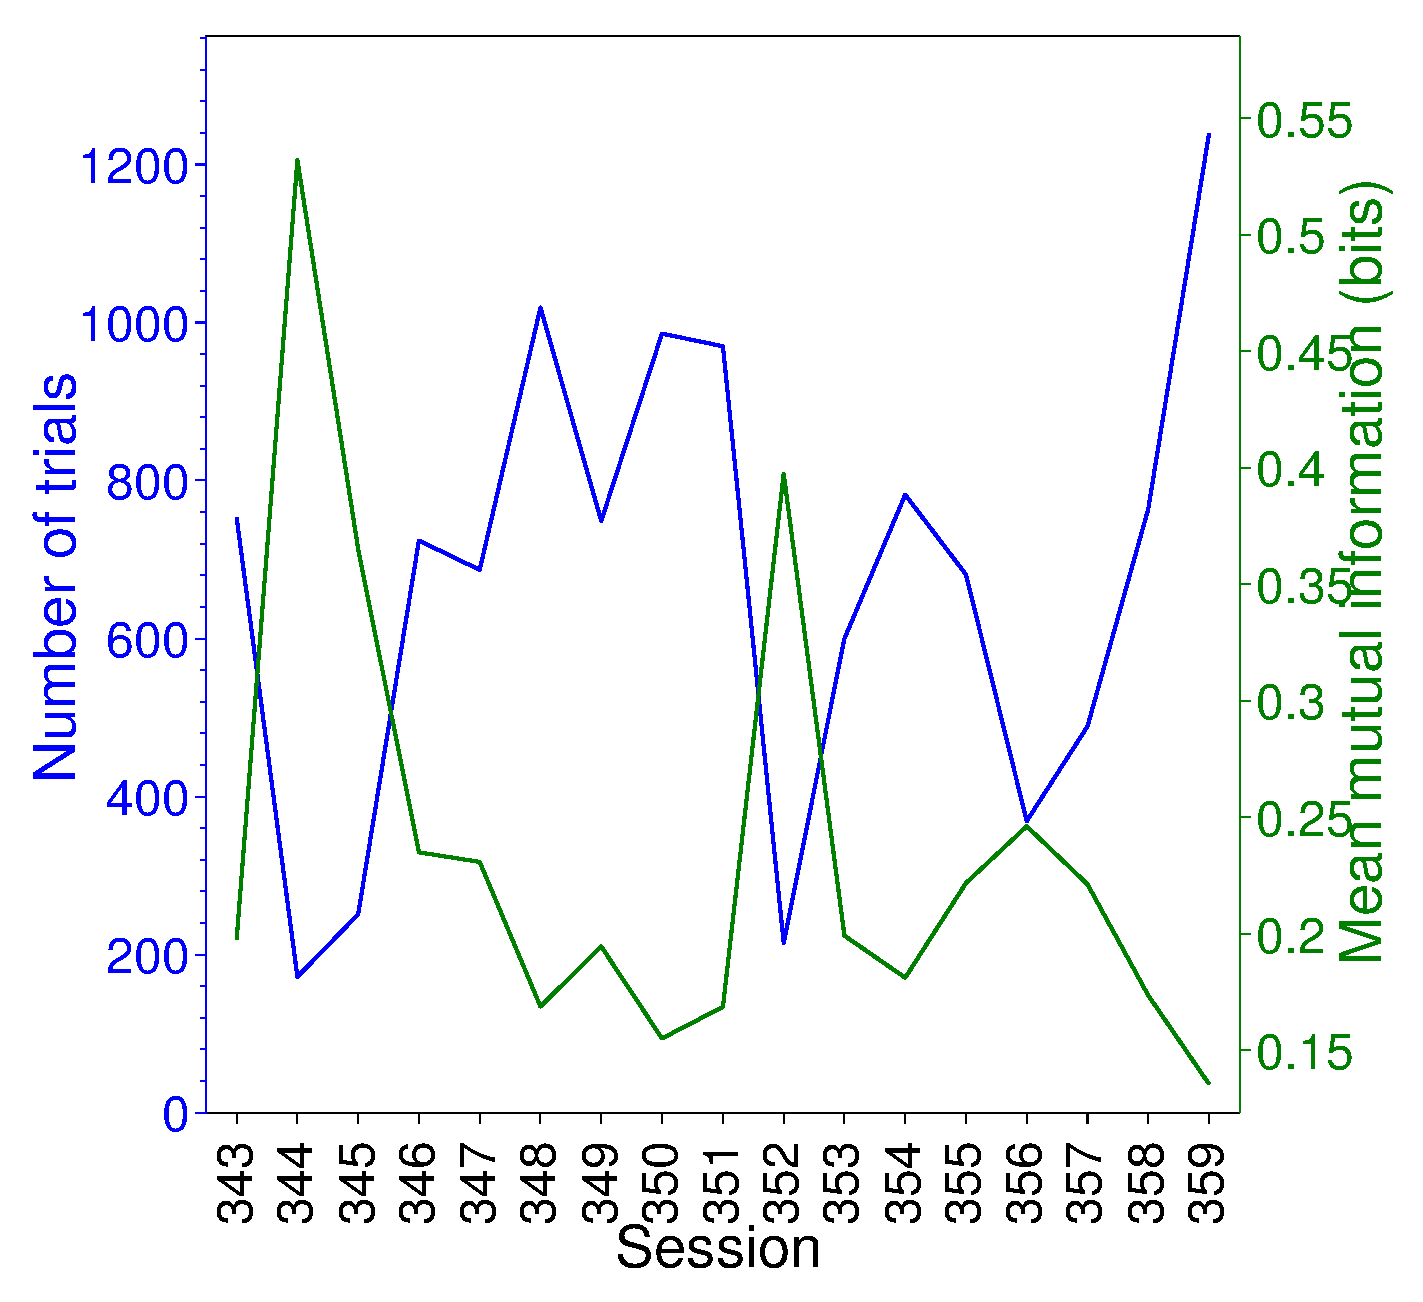
\includegraphics[width=\linewidth]{%
% % ./figs/ntrialsIandNindiv_blanco_v1_dr_naive_5bins_of_4ms_20120815T201856.eps}
% %     \end{subfigure}
% %     \begin{subfigure}[b]{0.5\linewidth}
% %         \centering
% %         \caption{M1 V4}
% %         \label{fig:IandNb4}
% %         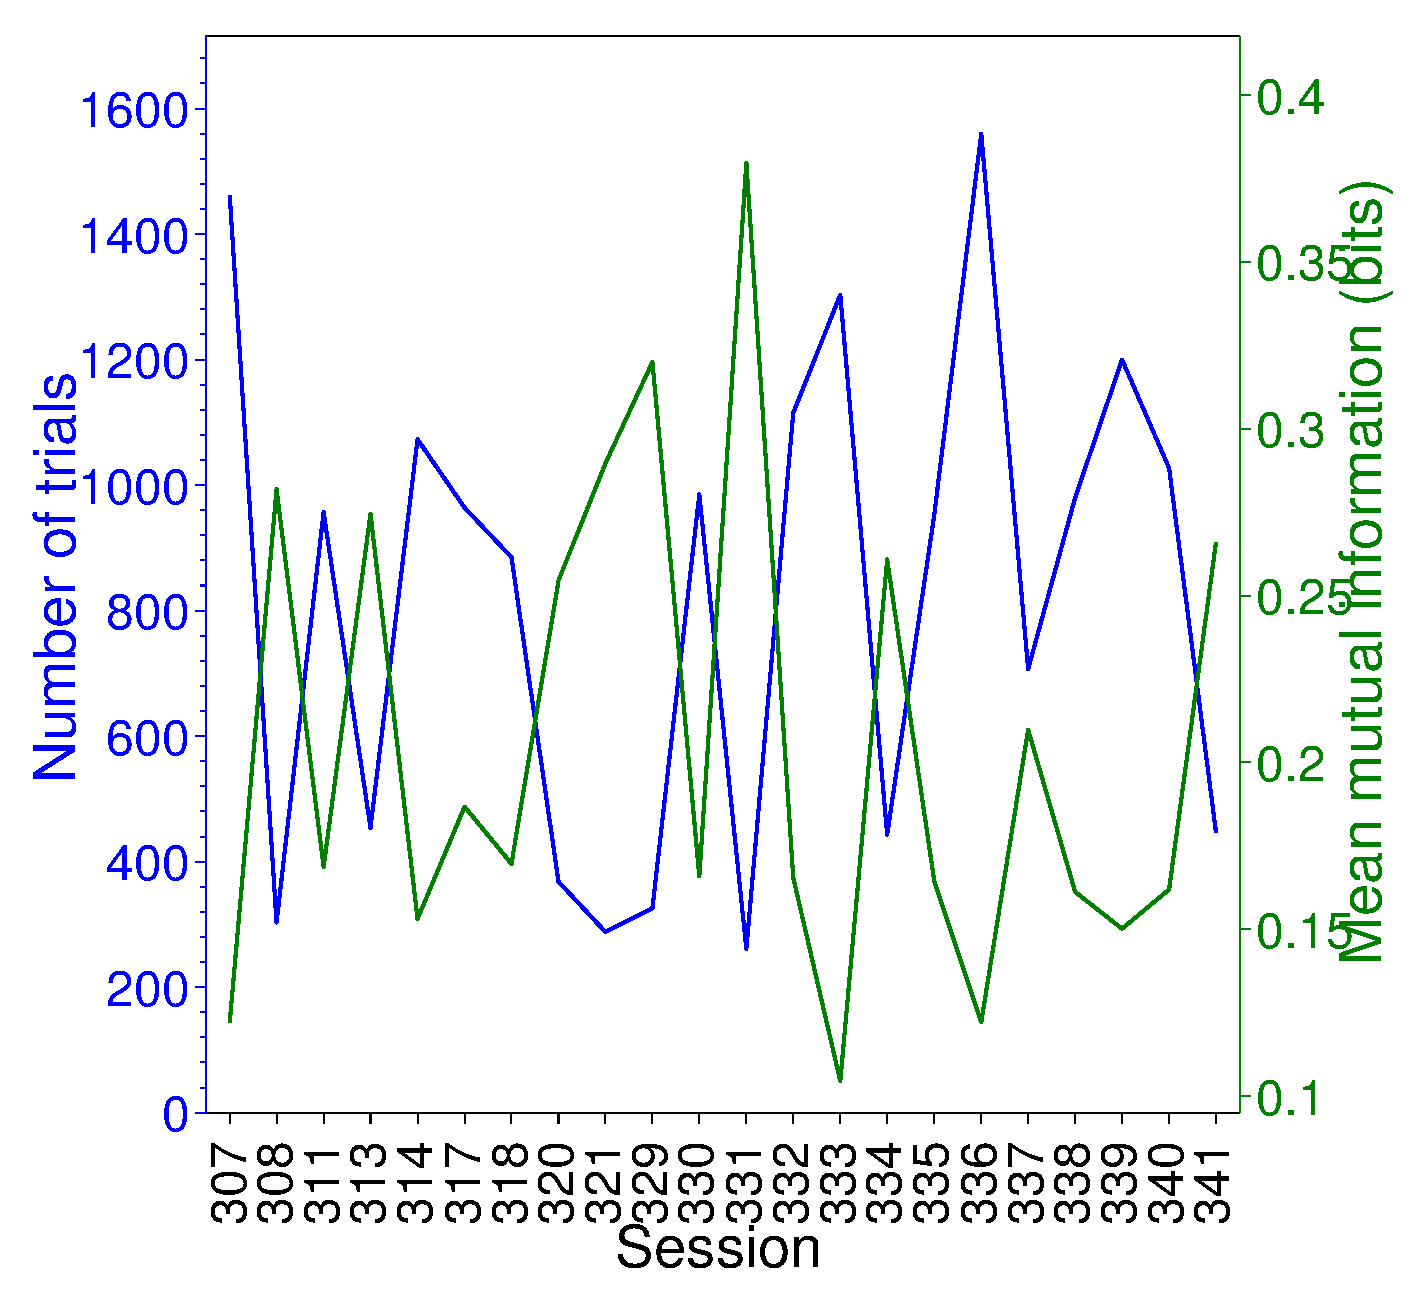
\includegraphics[width=\linewidth]{%
% % ./figs/ntrialsIandNindiv_blanco_v4_dr_naive_5bins_of_4ms_20120815T201856.eps}
% %     \end{subfigure}
% %     \\
% %     \begin{subfigure}[b]{0.5\linewidth}
% %         \centering
% %         \caption{M2 V1}
% %         \label{fig:IandNj1}
% %         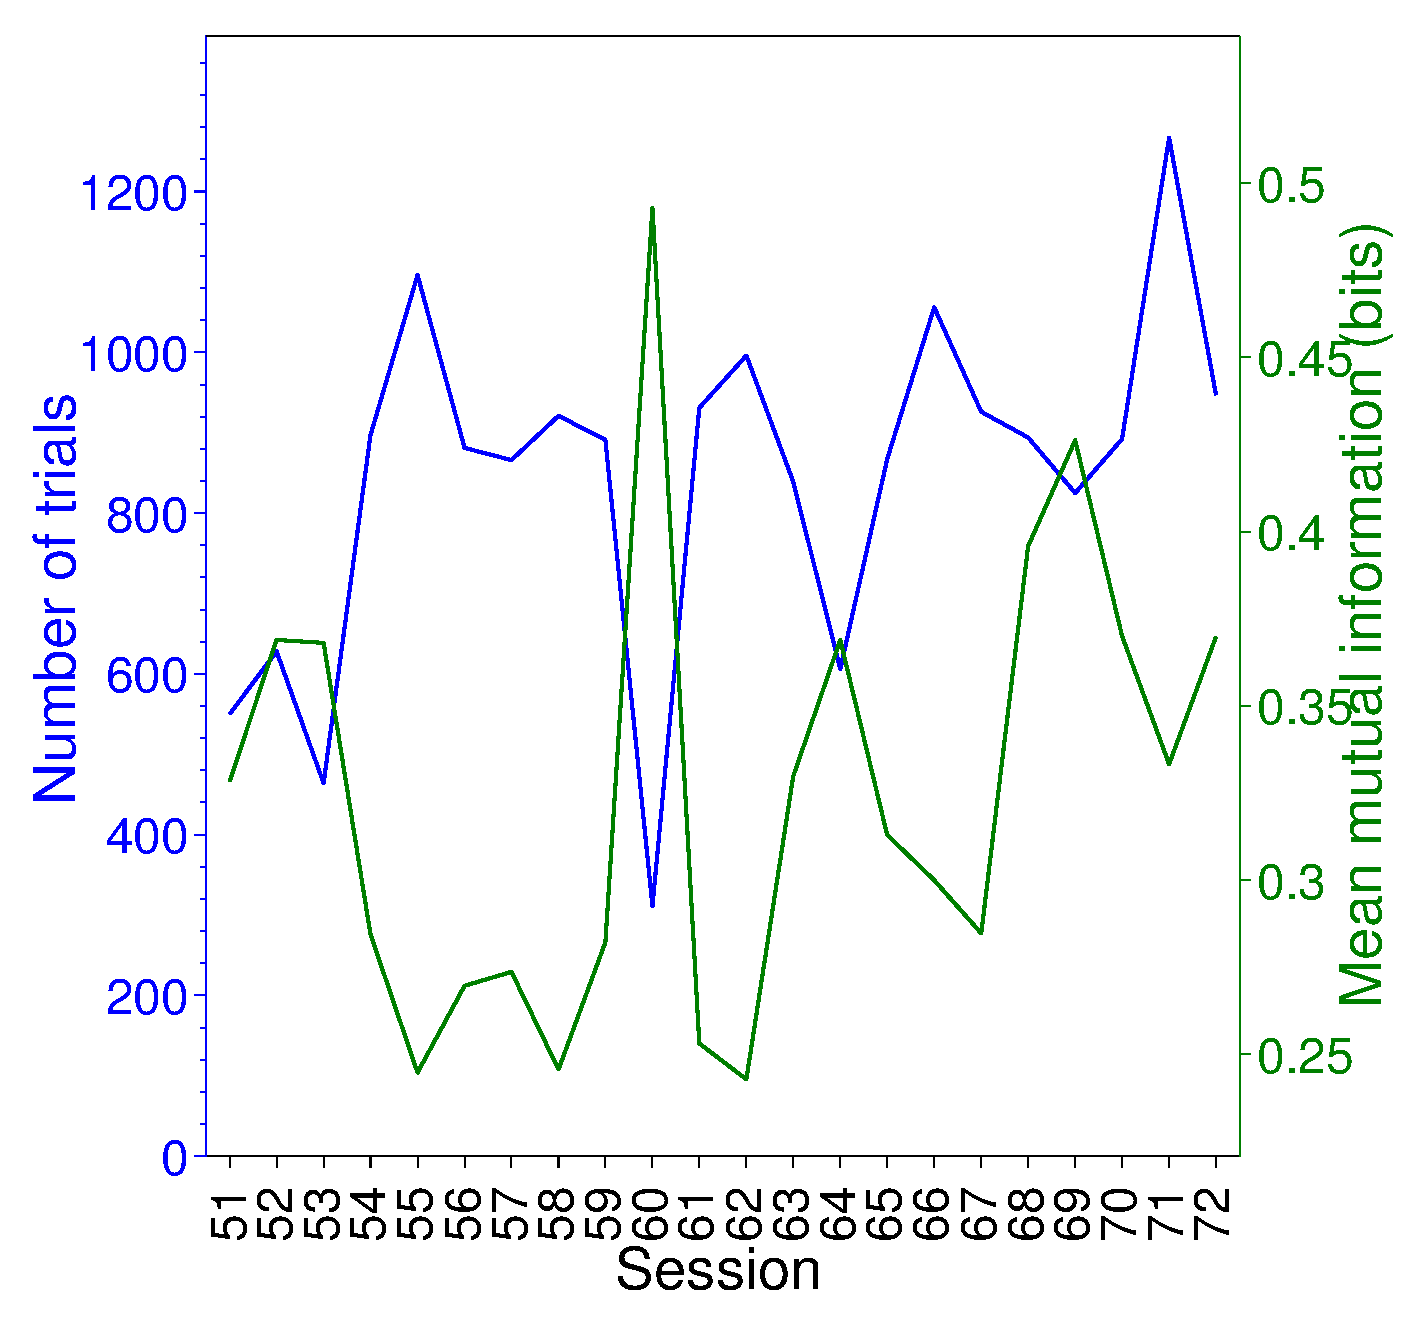
\includegraphics[width=\linewidth]{%
% % ./figs/ntrialsIandNindiv_jack_v1_dr_naive_5bins_of_4ms_20120815T201856.eps}
% %     \end{subfigure}
% %     \begin{subfigure}[b]{0.5\linewidth}
% %         \centering
% %         \caption{M2 V4}
% %         \label{fig:IandNj4}
% %         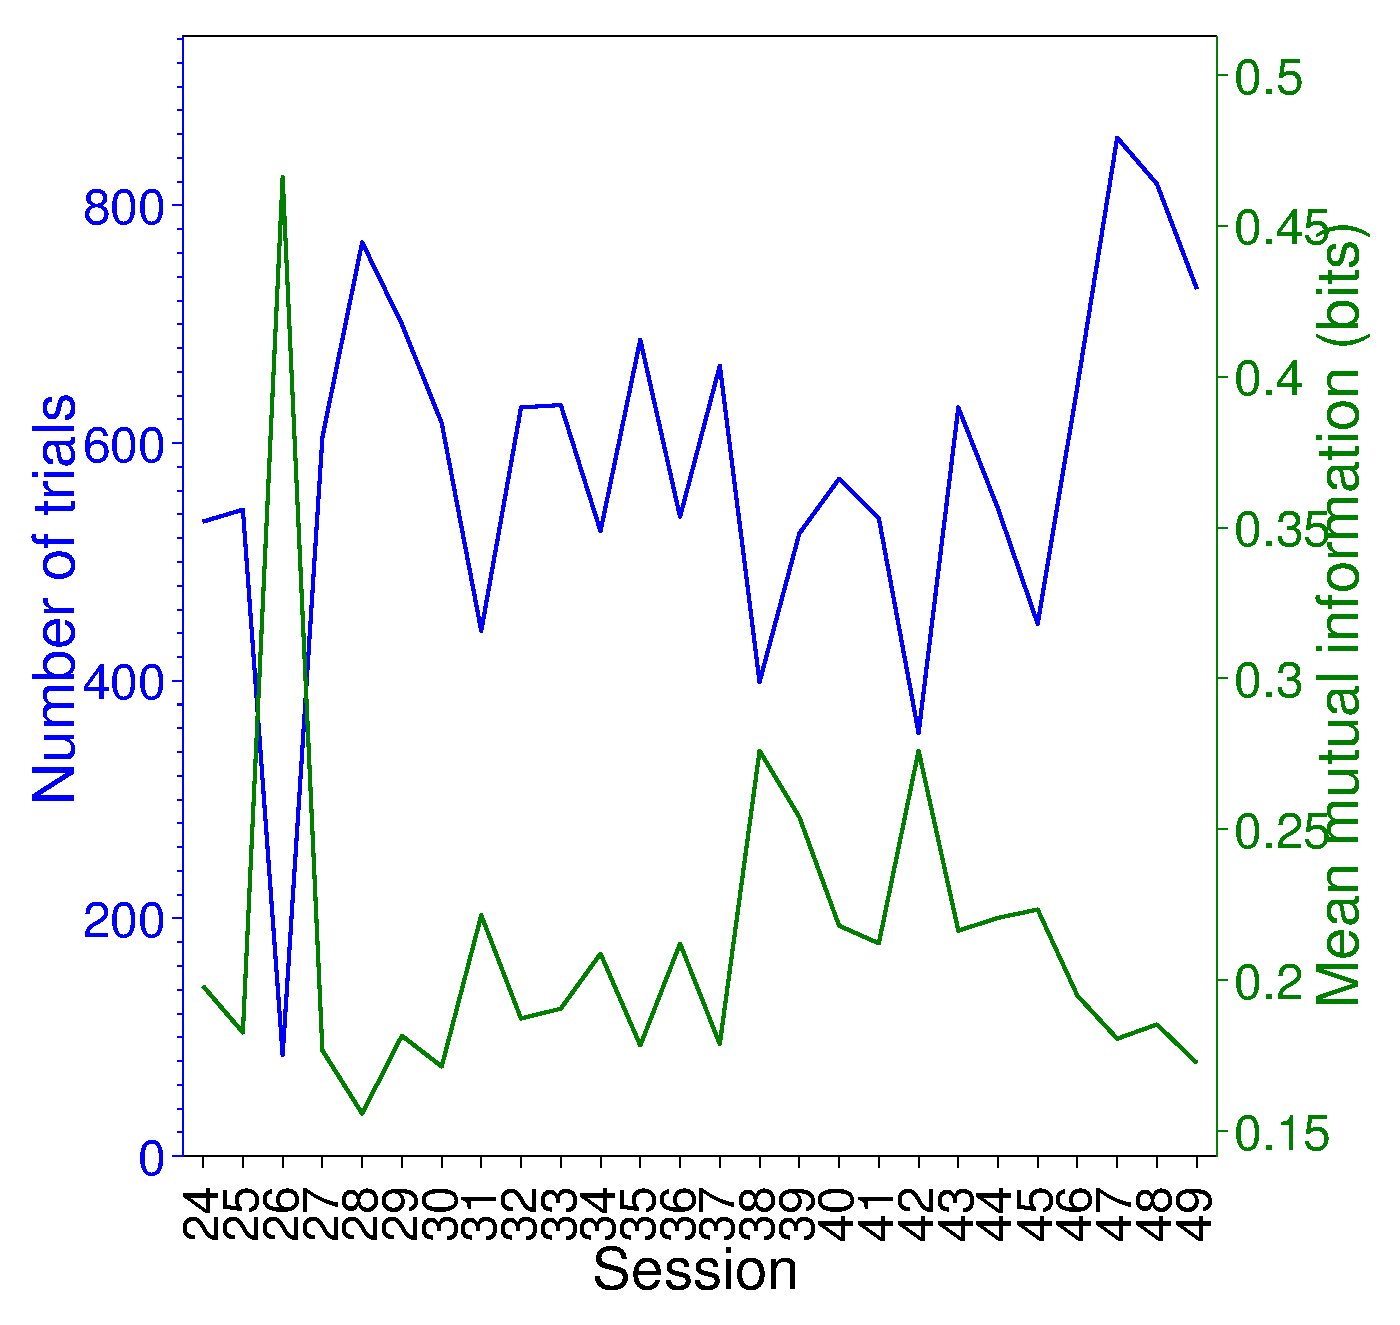
\includegraphics[width=\linewidth]{%
% % ./figs/ntrialsIandNindiv_jack_v4_dr_naive_5bins_of_4ms_20120815T201856.eps}
% %     \end{subfigure}
% %     \caption{Mutual information seems to be anti-correlated with the number of trials in the session. The number of correctly responded trials in each session is plotted on top of the mean information in individual sessions. The mutual information is the ``plug-in estimate'', not corrected for bias, and averaged across the whole period of test stimulus presentation.
% % %There is a missing data point for M2 V4 because in one session there were not enough trials per condition for the QE algorithm to function.
% % }
% %     \label{fig:IandN}
% % \end{figure}

Fig.~\ref{fig:IandN} shows that the changes in the measured mutual information are dominated by the number of trials in the session, not by increases with perceptual learning (corresponding to increments in the session number).
The only exception to this rule seems to be for M2 V1, shown in Fig.~\ref{fig:IandNj1}, where the information increases with learning despite an increase in the number of trials per session over this period.

% ./figs/ntrialsIvsinvNcombindiv_blanco_v1_20120812T164553.eps
% ./figs/ntrialsIvsinvNcombindiv_blanco_v4_20120812T164553.eps
% ./figs/ntrialsIvsinvNcombindiv_jack_v1_20120812T164553.eps
% ./figs/ntrialsIvsinvNcombindiv_jack_v4_20120812T164553.eps
% 
% ./figs/ntrialsIvsinvNcombindiv_blanco_v1_5bins_of_4ms_20120815T204808.eps
% ./figs/ntrialsIvsinvNcombindiv_blanco_v4_5bins_of_4ms_20120815T204808.eps
% ./figs/ntrialsIvsinvNcombindiv_jack_v1_5bins_of_4ms_20120815T204808.eps
% ./figs/ntrialsIvsinvNcombindiv_jack_v4_5bins_of_4ms_20120815T204808.eps
% 
% % \begin{figure}[htbp]
% %     \begin{subfigure}[b]{0.5\linewidth}
% %         \centering
% %         \caption{M1 V1}
% %         \label{fig:IvNb1}
% %         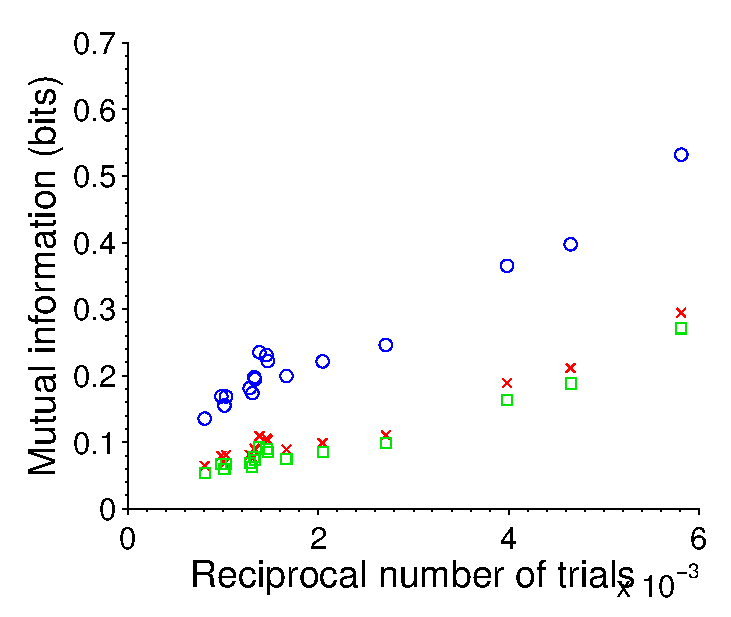
\includegraphics[width=\linewidth]{%
% % ./figs/ntrialsIvsinvNcombindiv_blanco_v1_5bins_of_4ms_20120815T204808.eps}
% %     \end{subfigure}
% %     \begin{subfigure}[b]{0.5\linewidth}
% %         \centering
% %         \caption{M1 V4}
% %         \label{fig:IvNb4}
% %         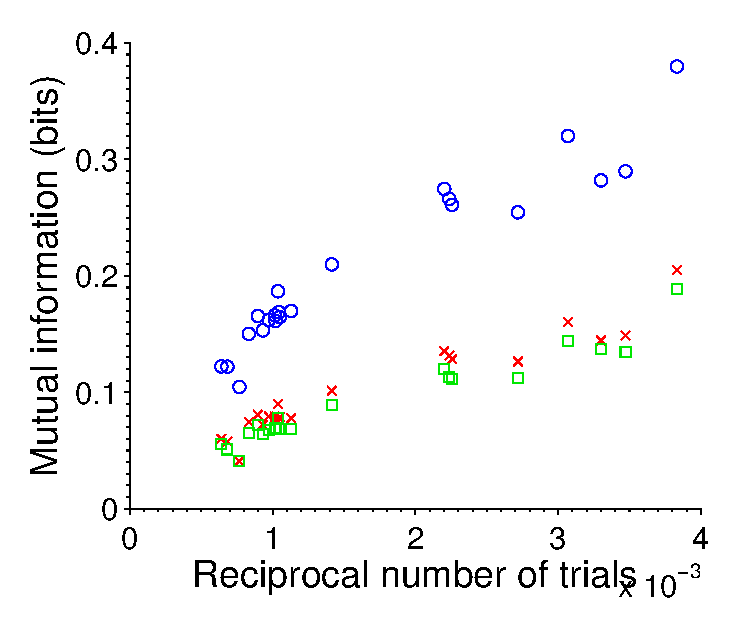
\includegraphics[width=\linewidth]{%
% % ./figs/ntrialsIvsinvNcombindiv_blanco_v4_5bins_of_4ms_20120815T204808.eps}
% %     \end{subfigure}
% %     \\
% %     \begin{subfigure}[b]{0.5\linewidth}
% %         \centering
% %         \caption{M2 V1}
% %         \label{fig:IvNj1}
% %         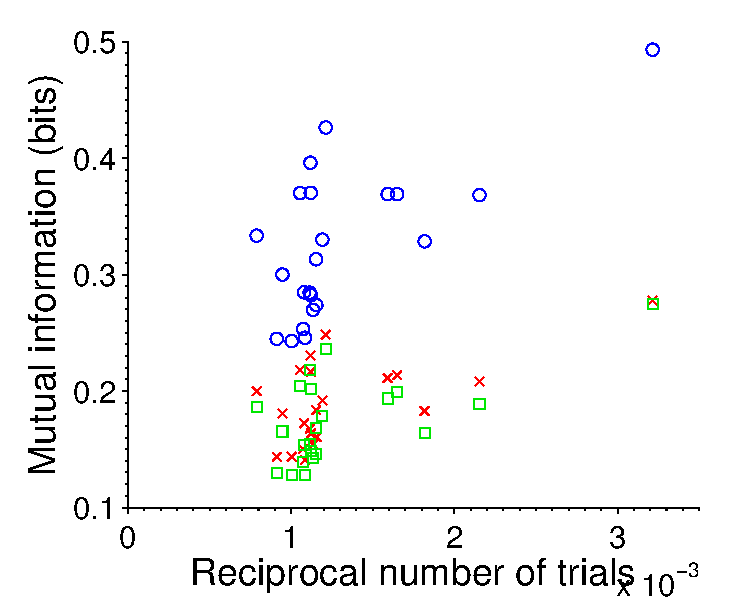
\includegraphics[width=\linewidth]{%
% % ./figs/ntrialsIvsinvNcombindiv_jack_v1_5bins_of_4ms_20120815T204808.eps}
% %     \end{subfigure}
% %     \begin{subfigure}[b]{0.5\linewidth}
% %         \centering
% %         \caption{M2 V4}
% %         \label{fig:IvNj4}
% %         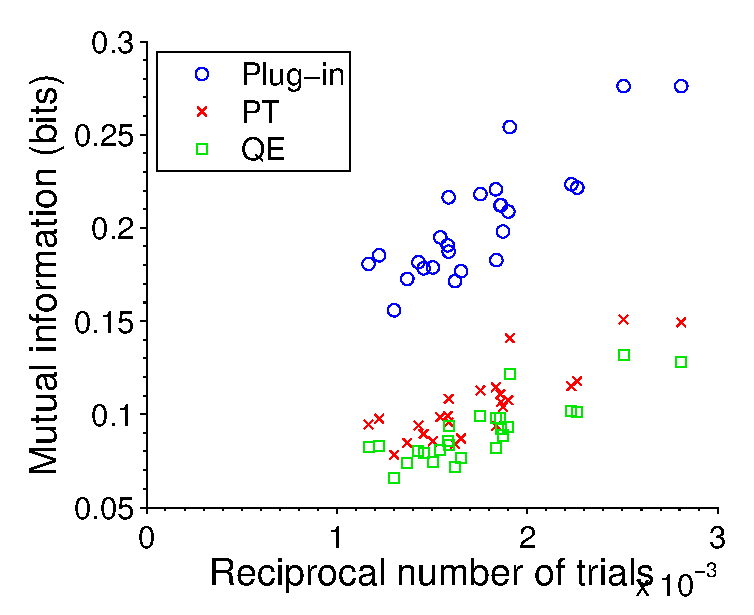
\includegraphics[width=\linewidth]{%
% % ./figs/ntrialsIvsinvNcombindiv_jack_v4_5bins_of_4ms_20120815T204808.eps}
% %     \end{subfigure}
% %     \caption{Mutual information is inversely correlated with the number of trials in the session. The mutual information for a single session is averaged over all channels, and averaged over all times during stimulus presentation, and plotted against the reciprocal of the number of trials in the session ($\nicefrac{1}{N}$). Plug-in:~with no bias correction. PT:~using the Panzeri-Treves method to correct for bias \cite{Panzeri1996}. QE:~using quadratic extrapolation for bias correction \cite{Strong1998}.
% % %There is a missing data point for M2 V4 because in one session there were not enough trials per condition for the QE algorithm to function.
% % }
% %     \label{fig:IvN}
% % \end{figure}

In particular, the measured value for the mutual information is strongly correlated with the reciprocal of the number of trials in the session (Fig.~\ref{fig:IvN}). The correlation is still very strong even if we use one of the two bias correction techniques. As discussed above, for M2 V1 the number of trials per session and the measured information  are both correlated with time, which reduces the correlation observed in Fig.~\ref{fig:IvNj1}.

The problem is that although PT and QE both do a reasonable attempt at removing the bias, they are not perfect and some bias will remain. As the bias is dependent on the number of trials, it is unsurprising the remaining bias follows the same dependency.
In particular, in the asymptotic regime the leading term in the expansion of $I_{\text{measured}}$ is known to be proportional \cite{Treves1995} to $\nicefrac{1}{N}$; the same relationship observed here.

In particular, the difficult faced is changes due to perceptual learning which are of interest may only be slight, but the the number of trials per session varies five-fold: from 250 up to 1250. Consequently it is unsurprising that the observed differences in information day-to-day are dominated by the number of trials.

% %----------------------------------------------------------------------------------------------------------------------
% \subsection{Results}
% 
% %----------------------------------------------------------------------------------------------------------------------
% \chapter{Information Theoretic Analysis (trial-wise)}
% %----------------------------------------------------------------------------------------------------------------------

%----------------------------------------------------------------------------------------------------------------------
\FloatBarrier
\subsubsection{Trial-based analysis}

To counter the correlation between measured information and number of trials, an obvious solution is to use the same number of trials for every computation. We now consider how many trials should be taken at once to obtain a reasonably reliable estimate.

Some rules-of-thumb for the number of trials are offered by \cite{Panzeri2007}.
Let $\overline{R}$ denote the number of possible response codes.
Then, for the plug-in estimate of mutual information, we need to have at least $N_S \ge 2^{32} \, \overline{R}$ trials per stimulus,
whilst if the PT or QE bias correction methods are applied, we only need $N_S > 2 \, \overline{R}$.

% The spike detection software was set to only detect spikes at least \unit[3]{ms} apart, and moreover, 
The probability of having two spikes within \unit[4]{ms} from a non-bursting neuron is very low. For example, a neuron with a high firing rate might fire at \unit[100]{Hz}, which means inter-spike intervals are typically around \unit[10]{ms} (and \unit[100]{Hz} is a high firing rate for the channels in our dataset).
Consequently any \unit[4]{ms} bin will realistically contain either 0 or 1 spikes, and the number of possible response codes in our spike timing code analysis with 5 bins each of \unit[4]{ms} is $\overline{R} = 2^5 = 32$. In comparison for a spike count code, if we assume spikes cannot be closer together than \unit[3]{ms}, there are between 0 and 7 spikes in any \unit[20]{ms} interval. Consequently there are $\overline{R} = 8$ possible response codes.

As we wish our analysis to work for both spike timing and spike count codes, using the above rules we need to use at least 64 trials per stimulus to get a reasonable estimate of the information with one of the bias correction methods in place.
Since there are 14 different stimuli, this means at least 896 trials in total are needed. This presents a dilemma, since most of the sessions are shorter than this, even when both correctly and incorrectly responded trials are included. Excluding sessions with fewer than 896 trials would severely limit the size of the dataset.
% and the patchwork of holes which would result would limit how much can be read into the results due to  which would result.

The solution found was to concatenate the sessions together and analyse groups of $N$ trials taken from multiple consecutive sessions.
The na\"{i}ve justification for this approach is a ``first-order approximation'' to perceptual learning would be that the monkey gets better at recognising the stimuli every-time they perceive it, and so the most important quantifier for the amount of perceptual learning which has taken place is the total number of trials the monkey has performed to date.

This rather basic assumption neglects several factors which influence the animal's performance, such as their mood during the particular training day; and factors which influence the animal's willingness to work (in turn influencing performance), which depends on their recent level of access to water (the reward used in the study). For instance, the animal performs less well on Mondays, which follows on from readily available water during the weekend.
Furthermore, the consolidation which occurs during sleep is commonly believed to be important to perceptual learning, and (as this only occurs between training sessions) this effect is completely ignored by this approach.

However, the session-concatenation approach was attempted regardless, and a value of $N_S = 100$ trials per stimulus was chosen. Though there are enough trials available to use more and reduce the bias further, it is undesirable data from so many sessions at once.

As mentioned in Chap.~\ref{ch:exp}, a delayed repeat is used for any trials to which the animal does not correctly respond. Consequently, more difficult test stimuli (with contrasts close to the sample contrast) are presented significantly more frequently than easier stimuli.
For instance, when presented with the most difficult test stimuli, the animal will have a success rate only just above 50\% on the first day of the experiment, rising to around 70\% by the last day. For the easiest stimuli, the success rate will be nearly 100\% throughout.

Say we arrange all the trials into groups based on their stimulus, then take 100 subsequent trials from each of the groups to perform the analysis on. Due to the different number of trials per stimulus, it will not be long before the trials selected for each stimulus are from very different points in time and from different sessions.\footnote{Even if we only analyse the correctly responded trials, there is still a difference in the number of trials per stimulus due to a limit on the number of repeats of any test condition. The difference was negligible for M1, but accumulated to a 100 trial difference over all the sessions between the most and least correctly responded conditions for M2.}
To ensure all the trials are from when the animal has had the same amount of training, we can instead take a group of $S \cdot N_S = 14 \cdot 100 = 1400$ consecutive trials regardless of the stimulus presented and analysed. The differences in number of trials per stimulus are not particularly important, so long as there are always  enough.

All trials where the monkey completed the trial and gave a response (either correct or incorrect) were included in the analysis. Trials where the monkey did not complete the task by fixating and then providing a response as required were excluded.
Using both the correct and incorrectly responded trials means our distribution for $P(s)$ is the same as that presented to the monkey, and there are notably more trials available to perform the analysis on.

% Using 50 and 100 trials explored: not considerable difference between results. 100 shown for conciseness

%----------------------------------------------------------------------------------------------------------------------
\FloatBarrier
\subsubsection{Information in fine vs. coarse distinctions}

The difference between information about fine differences in contrast can be studied by only considering trials where the contrast presented is one of the middle 6 contrasts:
\{22, 25, 28, 32, 35, 40\}\% for V1 and
\{27, 28, 29, 31, 32, 33\}\% for V4.
To keep the dimensionality of the stimulus the same, this has been compared to the information across some more separated contrasts:
 \{5, 15, 22, 40, 50, 90\}\% for V1 and
\{10, 15, 20, 40, 50, 60\}\% for V4.
For V4, the group of coarsely differentiated contrasts is the outer most six contrasts, but for V1 the coarsely differentiated contrasts are alternate

%----------------------------------------------------------------------------------------------------------------------
\FloatBarrier
\subsubsection{Information in spike timing code vs. spike count code}

Because the possible responses in the spike timing and count codes have different dimensionality, they have different biases \cite{Panzeri2007} and it is not possible to compare them directly.
Consequently, to investigate how much more information there is in a spike timing based code we must consider a set of responses which have the same dimensionality, but lack the timing information.

To do this, the spike-timing response codes are taken, then shuffled across the 5 bins for every individual trial.%
\footnote{The shuffling of bins was performed using the open source Shuffle.m
available from \url{http://www.mathworks.com/matlabcentral/fileexchange/27076-shuffle}.}
Since the 5 bins are now in a random order, any information contained in their order is lost. To make ensure the estimate of the information in the spike-timing code with the timing information destroyed was reasonable, the information was measured for five different shuffles%
% \footnote{The five shuffles were performed with a random seed linked to microsecond of execution time.}
 and then the mean was taken.

The information contained in the \unit[4]{ms} level spike timing can then be found by subtracting the mean shuffled information from the unshuffled information.

%----------------------------------------------------------------------------------------------------------------------
\FloatBarrier
\subsubsection{Spontaneous activity}

To check whether changes in the data quality between sessions and other differences between sessions could be influencing the results, the information theoretic analysis was also applied the spontaneous activity from the animal.
In particular, the spontaneous activity from prior to the sample presentation was used, so the animal had not yet seen the test contrast.
Although monkey's brain activity cannot possibly contain any genuine information about the test contrast, we expect to measure a non-zero value for the information content due to the sampling bias.

%----------------------------------------------------------------------------------------------------------------------
%----------------------------------------------------------------------------------------------------------------------
%----------------------------------------------------------------------------------------------------------------------
\subsection{Results}

During the course of the analysis, results were inspected using PT and using QE for bias correction. The plots were similar in distribution, and each gave a similar magnitude for the information. However, PT gave visibly lower variance than QE, so only plots using PT are presented in this results section.
Using the $I_{\text{sh}}$ approach where the bias is corrected by shuffling bins across trials \cite{Montemurro2007} was also attempted for the spike timing code, but this increased the variance far too much to be of any practical use. The unexpectedly significant increase in variance is probably due to the nature of the correlations between the bins which are being shuffled.

We also compared some of the results both with the monitor artifact left in the data and with the dataset redacted to have it removed. There was no appreciable difference for any of the plots, though the amount of information went down when the data was redacted due to the loss of some of the spikes.

%----------------------------------------------------------------------------------------------------------------------
% \FloatBarrier
% \subsubsection{General Information plots}

Starting with V1, the first thing which is noticed in Figs.~\ref{fig:b1-trialwise} and \ref{fig:j1-trialwise} \ref{fig:b1-1x20tp4} and \ref{fig:b1-5x4tp4} is the large peak in information over the \unit[20]{ms} window starting at around \unit[40]{ms} after stimulus onset. This is due to the onset transient response, where there is a larger amount of neural activity, and this is also less variable than usual \cite{Muller2001}. A second, smaller peak from the ``rebound'' of the transient also occurs around \unit[100]{ms} after stimulus onset. Looking at the scalebars, we can see there is about 10 times as much information on average from the neurons in M2 than M1. This is probably due to differences in data quality between the two animals.

Comparing the information found using the spike timing code \ref{fig:b1-5x4tp4} with the spike count code \ref{fig:b1-1x20tp4}, it seems that there is significantly more information when the binned spike times are considered: there is three times as much information for the spike timing code for M1 and twice as much for M2. However, if we look at information in the spontaneous activity, this reveals we cannot trust this result, as the bias for the information from the spontaneous activity is much higher for the spike timing code than spike count.

For M1, aside from the transient, the information measured with the spike timing code from the spontaneous activity is about the same as the information from the test presentation, suggesting something has gone very wrong!

For the spike timing codes, there is a clear decrease in information with learning in M1, and a clear increase in information for M2. This is, however, present in both the test presentation activity and the spontaneous activity, suggesting it is not a genuine effect. This is believed to be due to a decrease in signal quality in the implants in M1, and possibly an increase in M2.
The increase is also seen in the spike count code for M2, but not to any real extent and it is doubtful that the result is significant.

The bias in the information for the spontaneous activity changes with time for the spike timing code, but does not for the spike count code.
Since any changes in the dataset are the same for both of these, this suggests there are too few trials for the spike timing code to give a reliable reading of the information. This would make sense because with an average of $N_S = 100$ trials per stimulus and a spike timing code with $\overline{R} = 32$, there are
on average $\nicefrac{N_S}{\overline{R}} = 3.125$ trials per response per stimulus,
whilst for a spike count code with $\overline{R} = 8$ there are on average $\nicefrac{N_S}{\overline{R}} = 12.5$ trials per response per stimulus.
Similarly if there we assume a minimum of $N_S = 64$ trials per stimulus, there are
at least $\nicefrac{N_S}{\overline{R}} > 2$ trials per response per stimulus for the spike timing code, and
at least $\nicefrac{N_S}{\overline{R}} > 8$ trials per response per stimulus for the spike count code.

The information in the spontaneous activity was subsequently computed with an average of $N_S = 200$ and with $N_S = 400$ trials per stimulus.
This means there is now $\nicefrac{N_S}{\overline{R}} > 8$ for the spike timing code, however precisely the same relationship was observed.
From this, we can conclude the problem is due to the inconsistencies between sessions. If the firing rate changes between two sessions, the probability distribution of the responses generated will change for each condition. This will not matter so much for the spike count code because there are only 8 possible responses, and even if there are only 250 trials in the session there should be at least 16 trials per condition, meeting the minimal requirements for the PT method to function.

The small bump in the information in the spontaneous activity around \unit[50]{ms} in Figs.~\ref{fig:b1-5x4tp4} and \ref{fig:j1-5x4tp4} will be due to an increase in activity from a transient response. This data is normalised so \unit[0]{ms} is when the animal begins fixating on the fixation target, and there will be a transient response after the animal saccades to the target. Although the increase in activity does not relate to the conditions used on the subsequent test presentation, the extra spikes will increase the variability of the response, and thus $H(\SET{R})$, which will not be cancelled out by an increase in $H(\SET{R}|\SET{S})$ for the same reasons the bias appears in the first place.

In short, the data for M1 V1 does not seem to be of good enough quality whilst M2 V1 does, and the information in the spike timing code cannot be trusted for either monkey.

%  ./figs/I_trialwise_blanco_v1_chmean23_s343-354,355.1,355.2,356-359_tp4_1bins_of_20ms_dr_pt_oc0_test_tc5-5-20,22-3-28,32,35-5-50,60,90_nt1400_ts350_rmvet1_rmvms0_pcolorhot_20120815T234452.png
% ./figs/I_trialwise_blanco_v1_chmean23_s343-354,355.1,355.2,356-359_tp1_1bins_of_20ms_dr_pt_oc0_test_tc5-5-20,22-3-28,32,35-5-50,60,90_nt1400_ts350_rmvet1_rmvms0_pcolorhot_20120815T234326.png
% ./figs/I_trialwise_blanco_v1_chmean23_s343-354,355.1,355.2,356-359_tp4_1bins_of_20ms_dr_pt_oc0_test_tc5-5-20,22-3-28,32,35-5-50,60,90_nt1400_ts350_rmvet1_rmvms1_pcolorhot_20120815T234741.png
% ./figs/I_trialwise_blanco_v1_chmean23_s343-354,355.1,355.2,356-359_tp1_1bins_of_20ms_dr_pt_oc0_test_tc5-5-20,22-3-28,32,35-5-50,60,90_nt1400_ts350_rmvet1_rmvms1_pcolorbp_20120816T175451.png
% ./figs/I_trialwise_blanco_v1_chmean23_s343-354,355.1,355.2,356-359_tp4_5bins_of_4ms_dr_pt_oc0_test_tc5-5-20,22-3-28,32,35-5-50,60,90_nt1400_ts350_rmvet1_rmvms1_pcolorhot_20120815T234513.png
% ./figs/I_trialwise_blanco_v1_chmean23_s343-354,355.1,355.2,356-359_tp1_5bins_of_4ms_dr_pt_oc0_test_tc5-5-20,22-3-28,32,35-5-50,60,90_nt1400_ts350_rmvet1_rmvms1_pcolorbp_20120816T175423.png

% % \cleartoevenpage

% % \begin{figure}[htbp]
% % %     \begin{subfigure}[b]{0.5\linewidth}
% % %         \centering
% % %         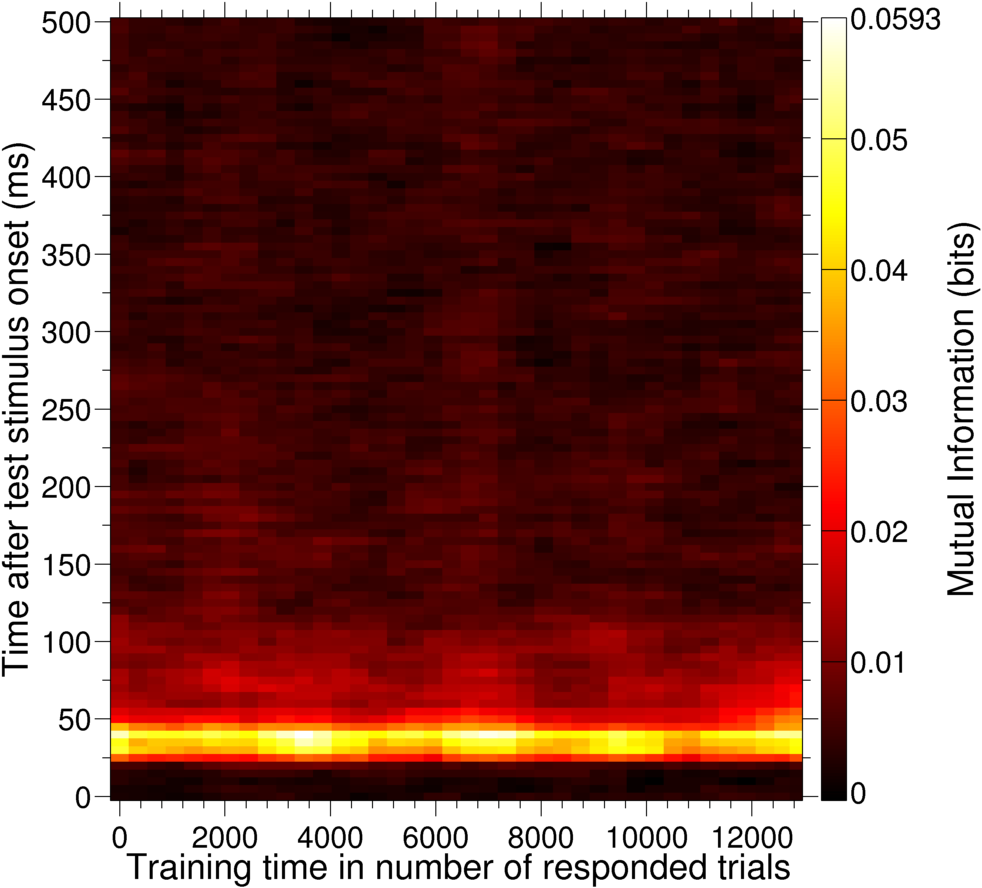
\includegraphics[scale=.25]{%
% % % ./figs/I_trialwise_blanco_v1_chmean23_s343-354,355.1,355.2,356-359_tp4_1bins_of_20ms_dr_pt_oc0_test_tc5-5-20,22-3-28,32,35-5-50,60,90_nt1400_ts350_rmvet1_rmvms0_pcolorhot_20120815T234452.png}
% % %         \caption{}
% % %         \label{fig:b1-1x20tp4ma}
% % %     \end{subfigure}
% % %     ~~
% % %     \begin{subfigure}[b]{0.5\linewidth}
% % %         \centering
% % %         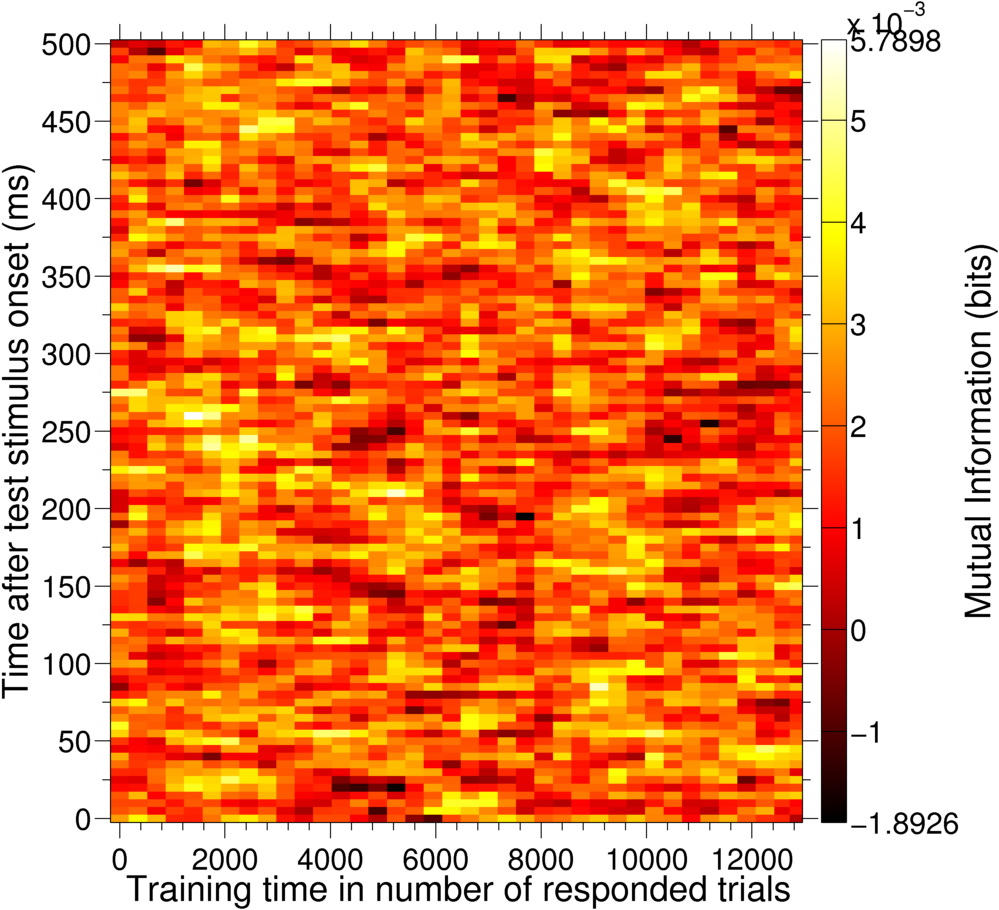
\includegraphics[scale=.25]{%
% % % ./figs/I_trialwise_blanco_v1_chmean23_s343-354,355.1,355.2,356-359_tp1_1bins_of_20ms_dr_pt_oc0_test_tc5-5-20,22-3-28,32,35-5-50,60,90_nt1400_ts350_rmvet1_rmvms0_pcolorhot_20120815T234326.png}
% % %         \caption{}
% % %         \label{fig:b1-1x20tp1ma}
% % %     \end{subfigure}
% % %     \\
% %     \begin{subfigure}[b]{0.5\linewidth}
% %         \centering
% %         \caption{}
% %         \label{fig:b1-1x20tp4}
% %         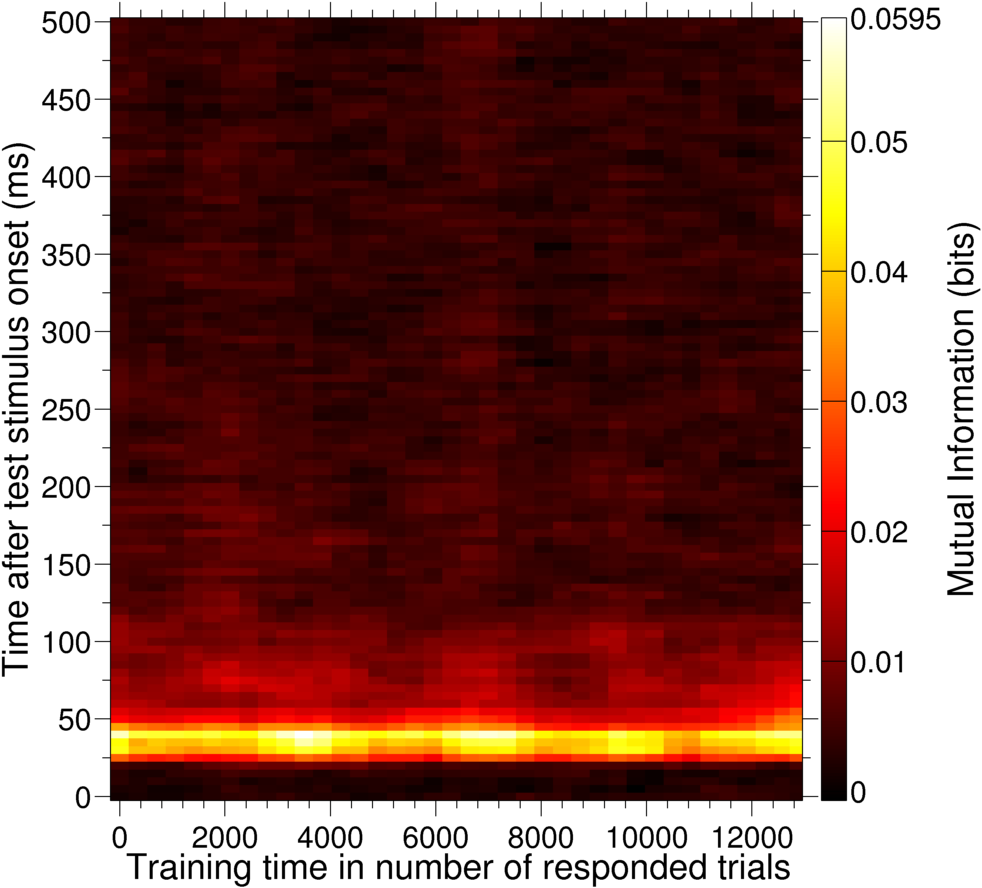
\includegraphics[scale=.25]{%
% % ./figs/I_trialwise_blanco_v1_chmean23_s343-354,355.1,355.2,356-359_tp4_1bins_of_20ms_dr_pt_oc0_test_tc5-5-20,22-3-28,32,35-5-50,60,90_nt1400_ts350_rmvet1_rmvms1_pcolorhot_20120815T234741.png}
% %     \end{subfigure}
% %     ~~
% %     \begin{subfigure}[b]{0.5\linewidth}
% %         \centering
% %         \caption{}
% %         \label{fig:b1-1x20tp1}
% %         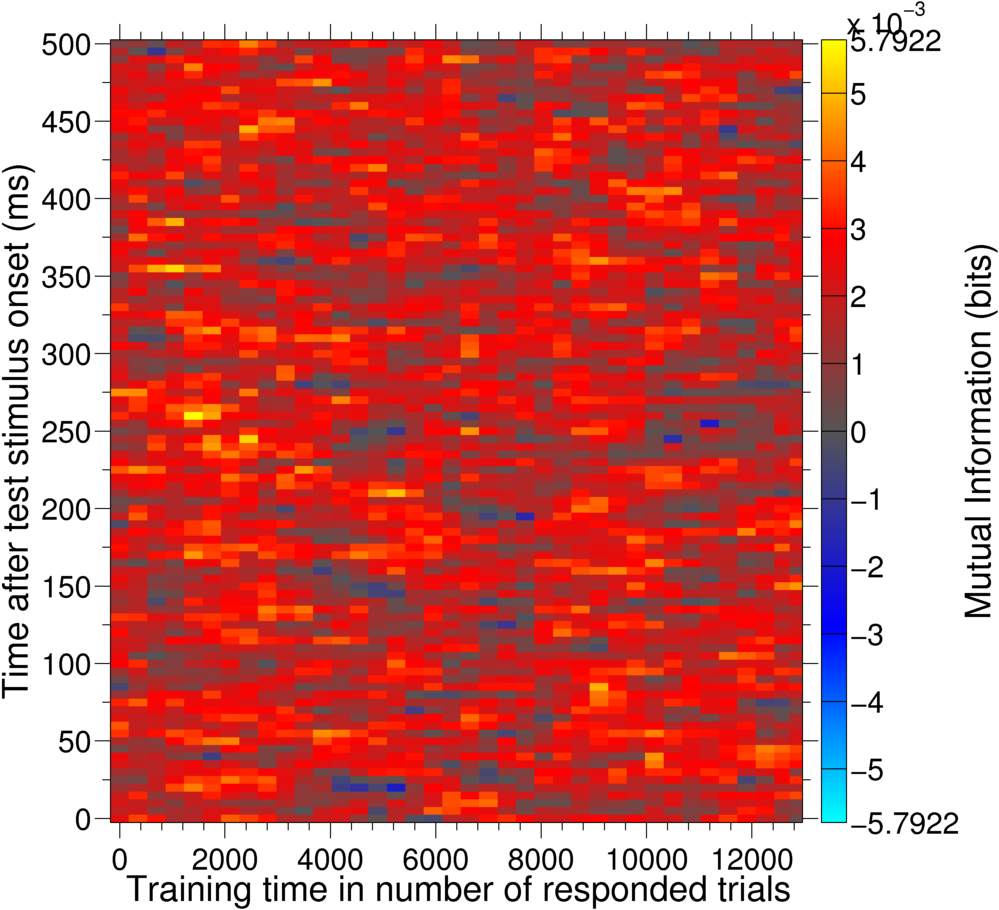
\includegraphics[scale=.25]{%
% % ./figs/I_trialwise_blanco_v1_chmean23_s343-354,355.1,355.2,356-359_tp1_1bins_of_20ms_dr_pt_oc0_test_tc5-5-20,22-3-28,32,35-5-50,60,90_nt1400_ts350_rmvet1_rmvms1_pcolorbp_20120816T175451.png}
% %     \end{subfigure}
% %     \\
% %     \begin{subfigure}[b]{0.5\linewidth}
% %         \centering
% %         \caption{}
% %         \label{fig:b1-5x4tp4}
% %         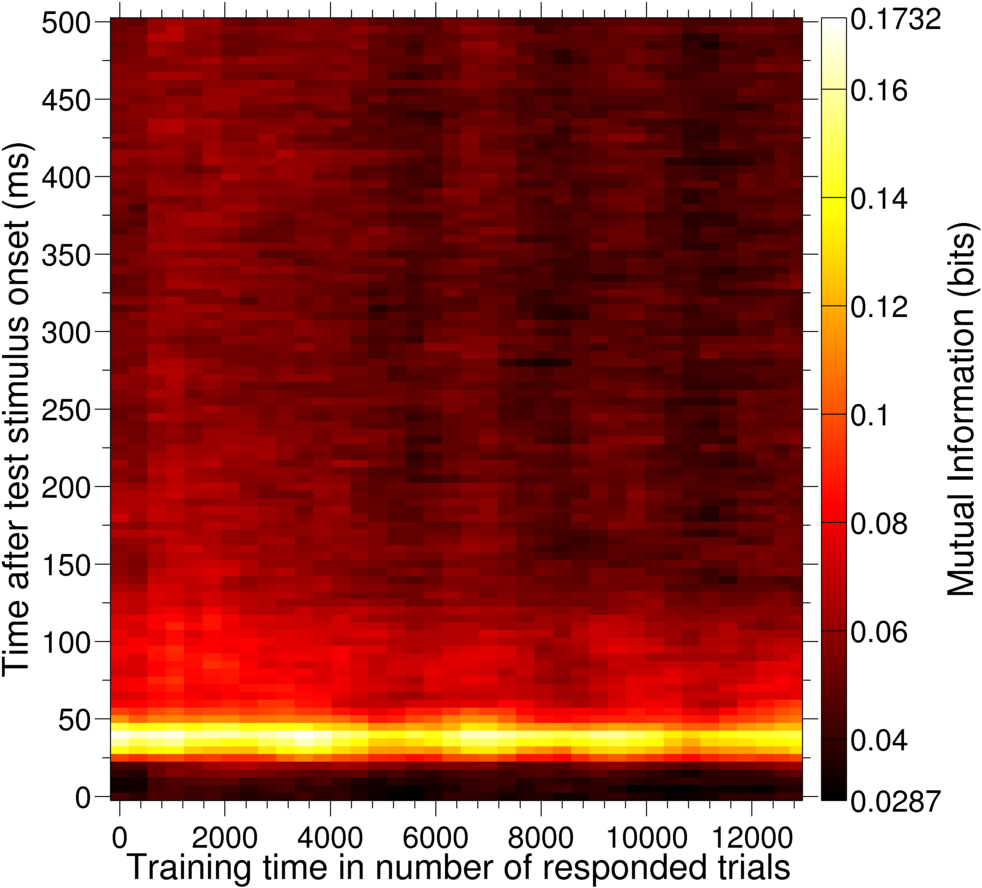
\includegraphics[scale=.25]{%
% % ./figs/I_trialwise_blanco_v1_chmean23_s343-354,355.1,355.2,356-359_tp4_5bins_of_4ms_dr_pt_oc0_test_tc5-5-20,22-3-28,32,35-5-50,60,90_nt1400_ts350_rmvet1_rmvms1_pcolorhot_20120815T234513.png}
% %     \end{subfigure}
% %     ~~
% %     \begin{subfigure}[b]{0.5\linewidth}
% %         \centering
% %         \caption{}
% %         \label{fig:b1-5x4tp1}
% %         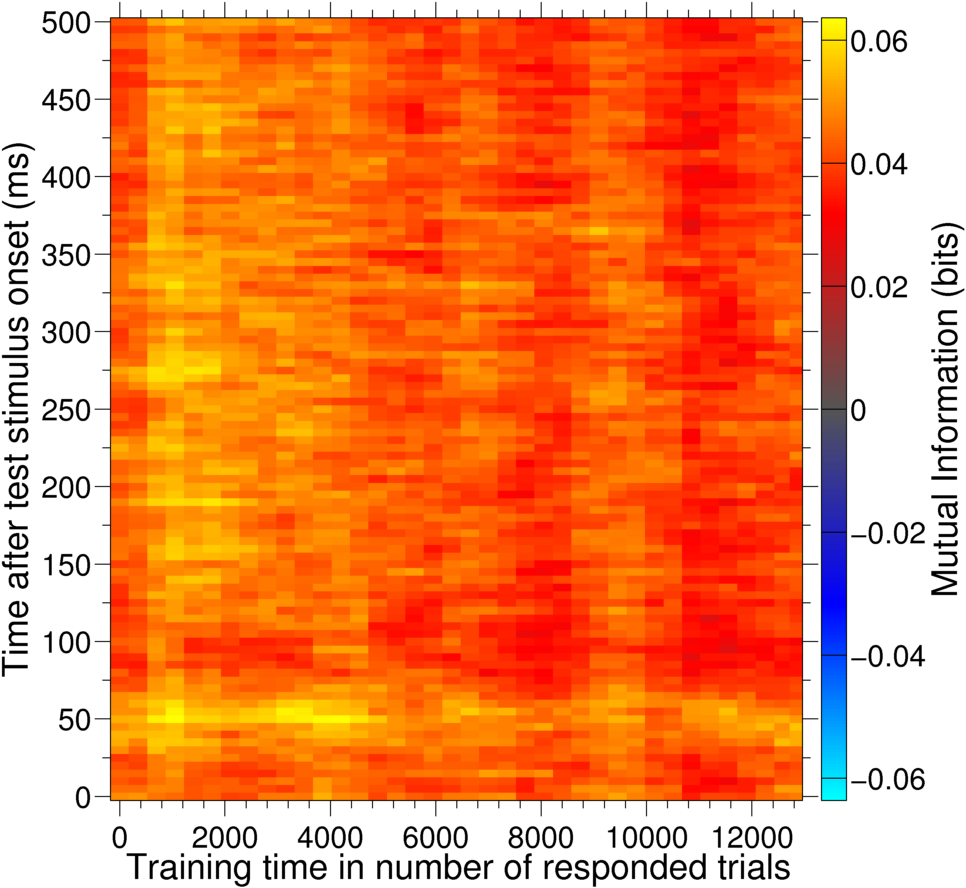
\includegraphics[scale=.25]{%
% % ./figs/I_trialwise_blanco_v1_chmean23_s343-354,355.1,355.2,356-359_tp1_5bins_of_4ms_dr_pt_oc0_test_tc5-5-20,22-3-28,32,35-5-50,60,90_nt1400_ts350_rmvet1_rmvms1_pcolorbp_20120816T175423.png}
% %     \end{subfigure}
% %     \caption{M1 V1: Mutual information between the test stimulus and \unit[20]{ms} of spiking activity, averaged across 23 channels.
% % The PT bias correction method was used in all estimates of the information, and the modification to the spiking data to remove the artifact as described in Sec.~\ref{sec:ma} was performed.
% % The neural code used in \ref{fig:b1-1x20tp4}, \ref{fig:b1-1x20tp1} is a spike count code, whilst in \ref{fig:b1-5x4tp4} and \ref{fig:b1-5x4tp1} it is a spike timing code where the \unit[20]{ms} window was subdivided into 5 bins each of \unit[4]{ms}.
% % In \ref{fig:b1-1x20tp4} and \ref{fig:b1-5x4tp4} the spike-train is taken from the test presentation part of the trial;
% % for \ref{fig:b1-1x20tp1} and \ref{fig:b1-5x4tp1} the spike-train is taken from spontaneous pre-stimulus activity.
% % The data is sampled in intervals of \unit[350]{trials} in the $x$-direction and \unit[5]{ms} in the $y$-direction, so there is significant correlation between any pair of pixels in the image with less than 4 pixels between them in either cartesian direction.
% % % In \ref{fig:b1-1x20tp4ma}, \ref{fig:b1-1x20tp4}, and \ref{fig:b1-5x4tp4}, the spike-train is taken from the test presentation part of the trial;
% % % for \ref{fig:b1-1x20tp1ma}, \ref{fig:b1-1x20tp1}, and \ref{fig:b1-5x4tp1}, the spike-train is taken from spontaneous pre-stimulus activity.
% % % In \ref{fig:b1-1x20tp4ma} and \ref{fig:b1-1x20tp1ma} no attempt was made to remove the monitor artifact from the raw data, whilst in the rest of the panels the data was modified to counter this as described in \ref{sec:ma}.
% % % \ref{fig:b1-1x20tp4ma}
% % % \ref{fig:b1-1x20tp1ma}
% % % \ref{fig:b1-1x20tp4}
% % % \ref{fig:b1-1x20tp1}
% % % \ref{fig:b1-5x4tp4}
% % % \ref{fig:b1-5x4tp1}
% % }
% %     \label{fig:b1-trialwise}
% % \end{figure}


% ./figs/I_trialwise_jack_v1_chmean25_s51-72_tp4_1bins_of_20ms_dr_pt_oc0_test_tc5-5-20,22-3-28,32,35-5-50,60,90_nt1400_ts350_rmvet1_rmvms0_pcolorhot_20120815T234410.png
% ./figs/I_trialwise_jack_v1_chmean25_s51-72_tp1_1bins_of_20ms_dr_pt_oc0_test_tc5-5-20,22-3-28,32,35-5-50,60,90_nt1400_ts350_rmvet1_rmvms0_pcolorhot_20120815T234245.png
% ./figs/I_trialwise_jack_v1_chmean25_s51-72_tp4_1bins_of_20ms_dr_pt_oc0_test_tc5-5-20,22-3-28,32,35-5-50,60,90_nt1400_ts350_rmvet1_rmvms1_pcolorhot_20120815T234701.png
% ./figs/I_trialwise_jack_v1_chmean25_s51-72_tp1_1bins_of_20ms_dr_pt_oc0_test_tc5-5-20,22-3-28,32,35-5-50,60,90_nt1400_ts350_rmvet1_rmvms1_pcolorbp_20120816T175411.png
% ./figs/I_trialwise_jack_v1_chmean25_s51-72_tp4_5bins_of_4ms_dr_pt_oc0_test_tc5-5-20,22-3-28,32,35-5-50,60,90_nt1400_ts350_rmvet1_rmvms1_pcolorhot_20120815T234434.png
% ./figs/I_trialwise_jack_v1_chmean25_s51-72_tp1_5bins_of_4ms_dr_pt_oc0_test_tc5-5-20,22-3-28,32,35-5-50,60,90_nt1400_ts350_rmvet1_rmvms1_pcolorbp_20120816T175343.png

% % \begin{figure}[htbp]
% % %     \begin{subfigure}[b]{0.5\linewidth}
% % %         \centering
% % %         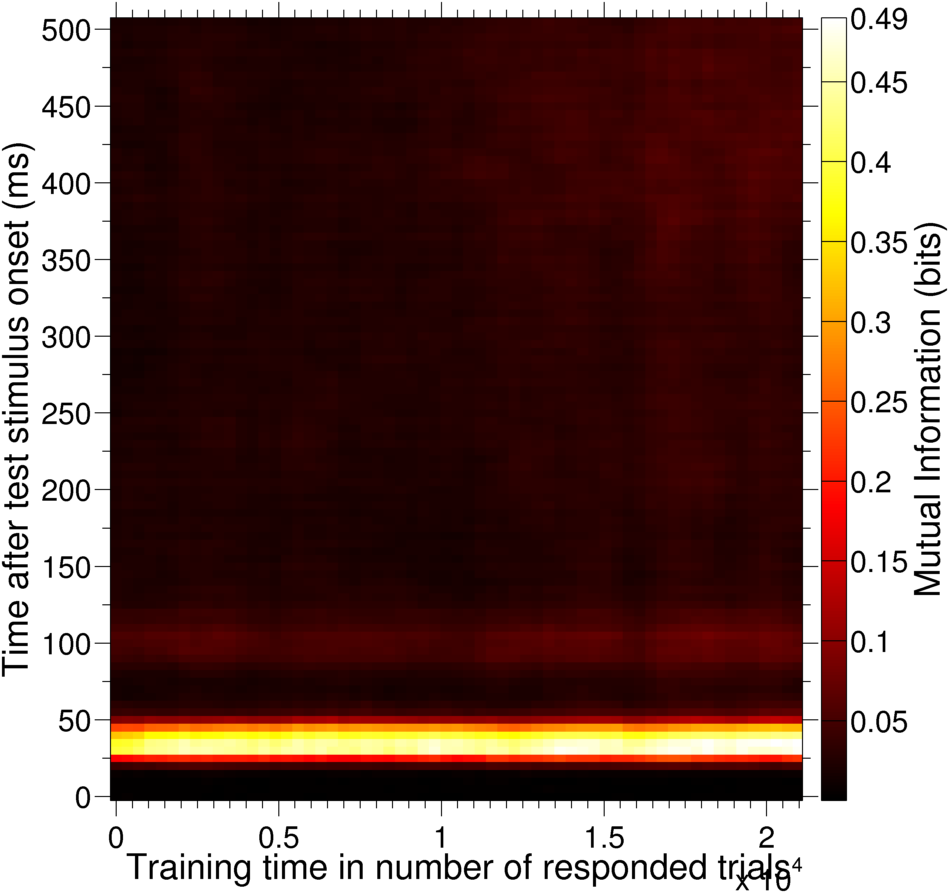
\includegraphics[scale=.25]{%
% % % ./figs/I_trialwise_jack_v1_chmean25_s51-72_tp4_1bins_of_20ms_dr_pt_oc0_test_tc5-5-20,22-3-28,32,35-5-50,60,90_nt1400_ts350_rmvet1_rmvms0_pcolorhot_20120815T234410.png}
% % %         \caption{}
% % %         \label{fig:j1-1x20tp4ma}
% % %     \end{subfigure}
% % %     ~~
% % %     \begin{subfigure}[b]{0.5\linewidth}
% % %         \centering
% % %         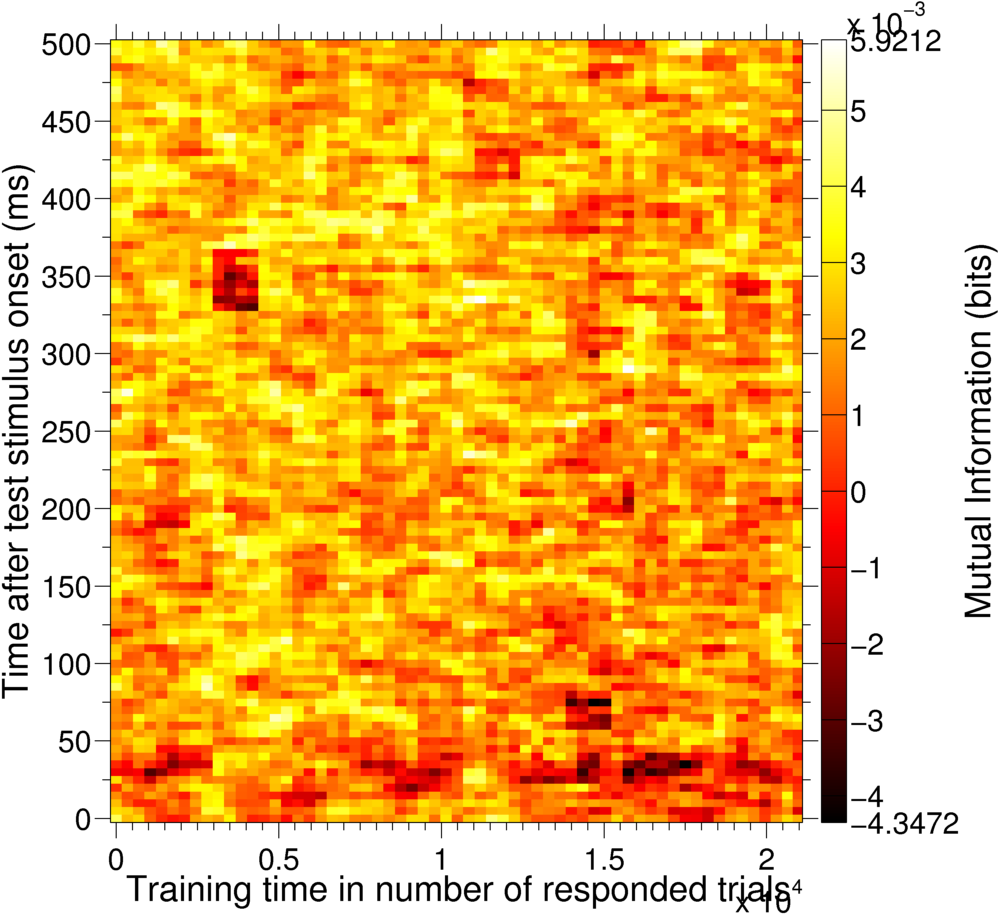
\includegraphics[scale=.25]{%
% % % ./figs/I_trialwise_jack_v1_chmean25_s51-72_tp1_1bins_of_20ms_dr_pt_oc0_test_tc5-5-20,22-3-28,32,35-5-50,60,90_nt1400_ts350_rmvet1_rmvms0_pcolorhot_20120815T234245.png}
% % %         \caption{}
% % %         \label{fig:j1-1x20tp1ma}
% % %     \end{subfigure}
% % %     \\
% %     \begin{subfigure}[b]{0.5\linewidth}
% %         \centering
% %         \caption{}
% %         \label{fig:j1-1x20tp4}
% %         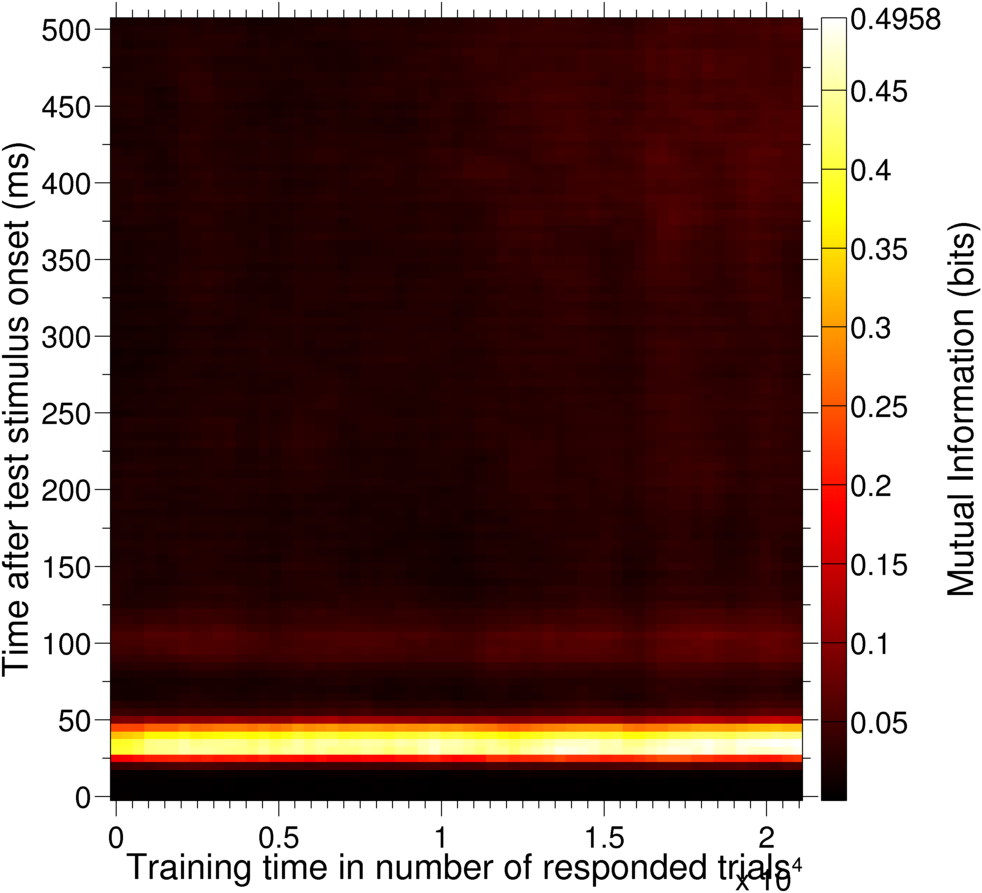
\includegraphics[scale=.25]{%
% % ./figs/I_trialwise_jack_v1_chmean25_s51-72_tp4_1bins_of_20ms_dr_pt_oc0_test_tc5-5-20,22-3-28,32,35-5-50,60,90_nt1400_ts350_rmvet1_rmvms1_pcolorhot_20120815T234701.png}
% %     \end{subfigure}
% %     ~~
% %     \begin{subfigure}[b]{0.5\linewidth}
% %         \centering
% %         \caption{}
% %         \label{fig:j1-1x20tp1}
% %         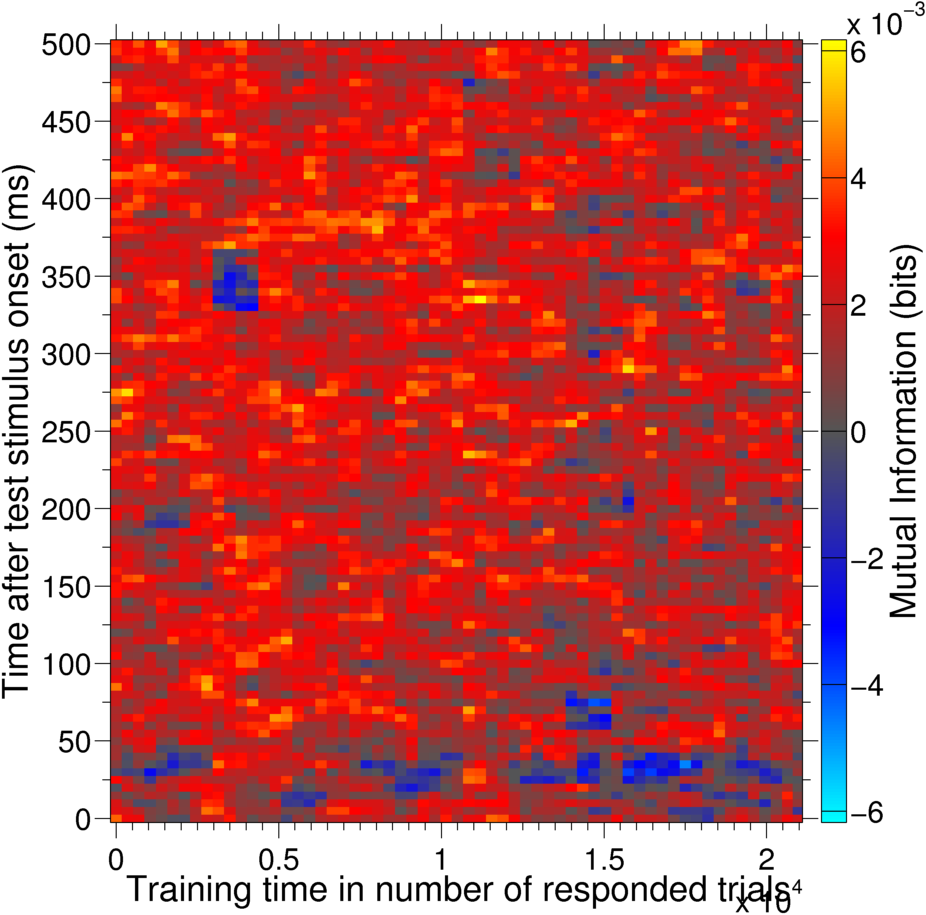
\includegraphics[scale=.25]{%
% % ./figs/I_trialwise_jack_v1_chmean25_s51-72_tp1_1bins_of_20ms_dr_pt_oc0_test_tc5-5-20,22-3-28,32,35-5-50,60,90_nt1400_ts350_rmvet1_rmvms1_pcolorbp_20120816T175411.png}
% %     \end{subfigure}
% %     \\
% %     \begin{subfigure}[b]{0.5\linewidth}
% %         \centering
% %         \caption{}
% %         \label{fig:j1-5x4tp4}
% %         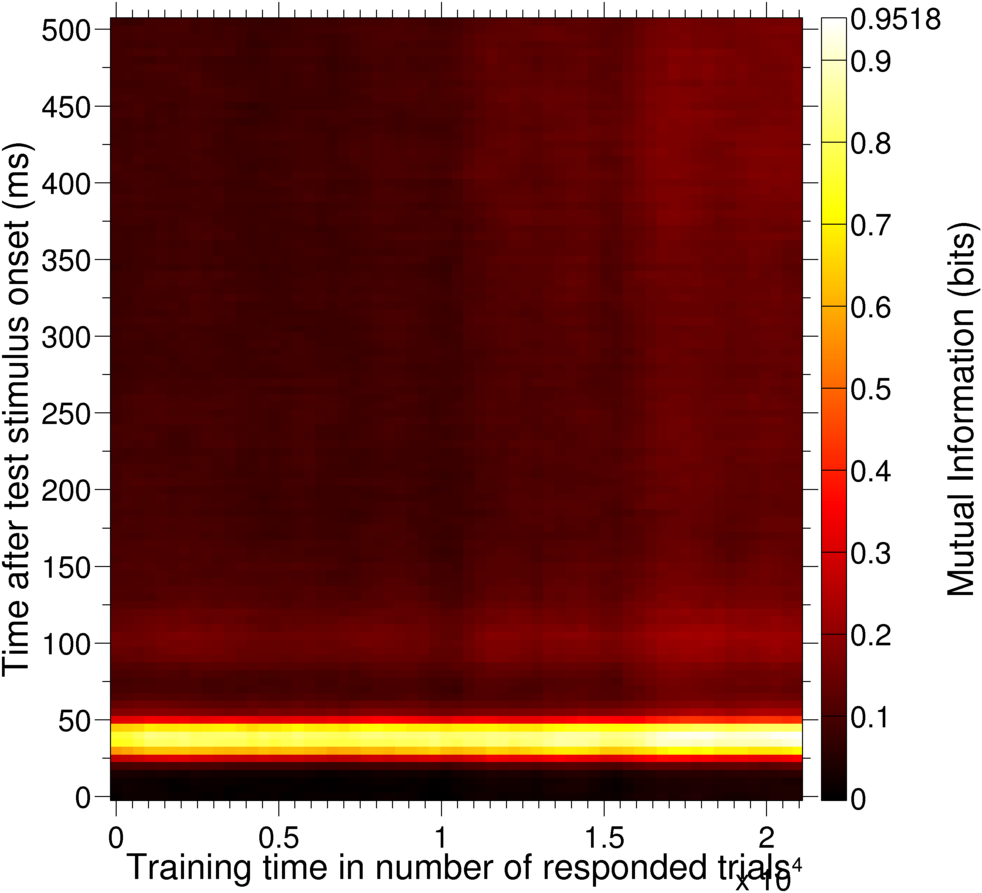
\includegraphics[scale=.25]{%
% % ./figs/I_trialwise_jack_v1_chmean25_s51-72_tp4_5bins_of_4ms_dr_pt_oc0_test_tc5-5-20,22-3-28,32,35-5-50,60,90_nt1400_ts350_rmvet1_rmvms1_pcolorhot_20120815T234434.png}
% %     \end{subfigure}
% %     ~~
% %     \begin{subfigure}[b]{0.5\linewidth}
% %         \centering
% %         \caption{}
% %         \label{fig:j1-5x4tp1}
% %         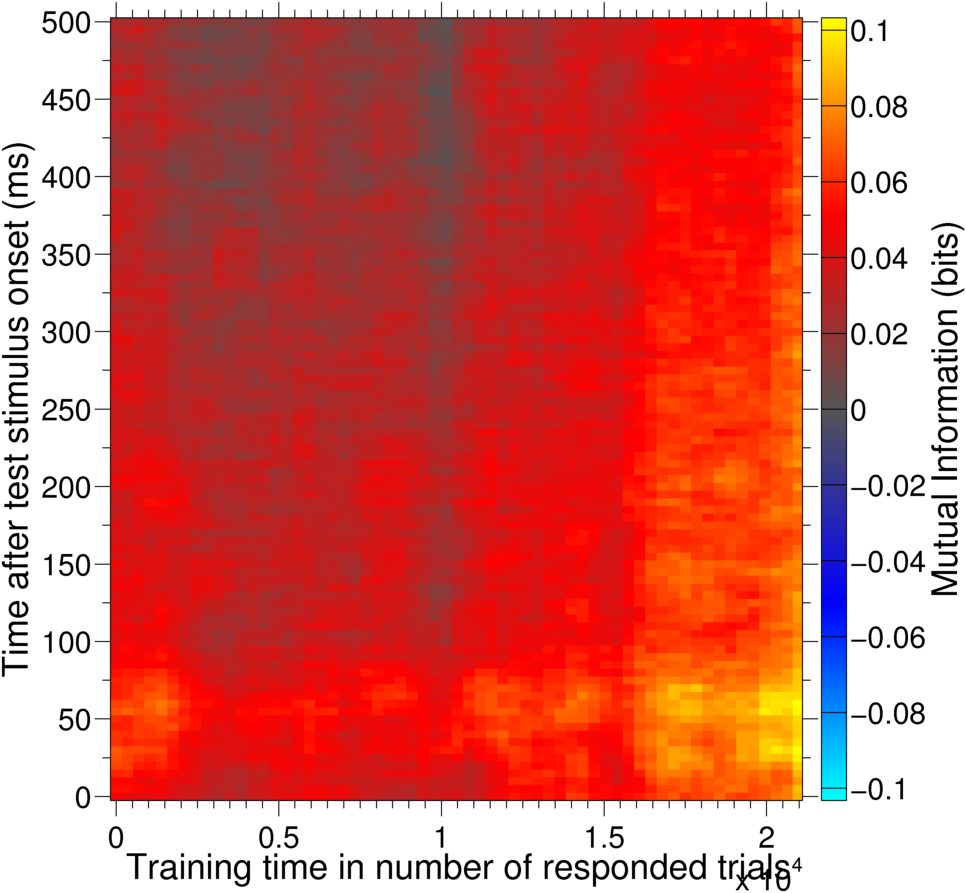
\includegraphics[scale=.25]{%
% % ./figs/I_trialwise_jack_v1_chmean25_s51-72_tp1_5bins_of_4ms_dr_pt_oc0_test_tc5-5-20,22-3-28,32,35-5-50,60,90_nt1400_ts350_rmvet1_rmvms1_pcolorbp_20120816T175343.png}
% %     \end{subfigure}
% %     \caption{M2 V1: Mutual information between the test stimulus and \unit[20]{ms} of spiking activity, averaged across 25 channels.
% % The PT bias correction method was used in all estimates of the information.
% % Panels \ref{fig:j1-1x20tp4}--\ref{fig:j1-5x4tp1} are the same as for Fig.~\ref{fig:b1-trialwise}.
% % % The neural code used in \ref{fig:j1-1x20tp4ma}--\ref{fig:j1-1x20tp1} is a spike count code, whilst in \ref{fig:j1-5x4tp4}, \ref{fig:j1-5x4tp1} it is a spike timing code where the \unit[20]{ms} window was subdivided into 5 bins each of \unit[4]{ms}.
% % % In \ref{fig:j1-1x20tp4ma}, \ref{fig:j1-1x20tp4}, and \ref{fig:j1-5x4tp4}, the spike-train is taken from the test presentation part of the trial;
% % % for \ref{fig:j1-1x20tp1ma}, \ref{fig:j1-1x20tp1}, and \ref{fig:j1-5x4tp1}, the spike-train is taken from spontaneous pre-stimulus activity.
% % % In \ref{fig:j1-1x20tp4ma} and \ref{fig:j1-1x20tp1ma} no attempt was made to remove the monitor artifact from the raw data, whilst in the rest of the panels the data was modified to counter this as described in \ref{sec:ma}.
% % % \ref{fig:j1-1x20tp4ma}
% % % \ref{fig:j1-1x20tp1ma}
% % % \ref{fig:j1-1x20tp4}
% % % \ref{fig:j1-1x20tp1}
% % % \ref{fig:j1-5x4tp4}
% % % \ref{fig:j1-5x4tp1}
% % }
% %     \label{fig:j1-trialwise}
% % \end{figure}

% ./figs/I_trialwise_blanco_v4_chmean31_s307,308,311,313,314,317,318,320,321,329-341_tp4_1bins_of_20ms_dr_pt_oc0_test_tc10-5-25,27-29,31-33,35,40-10-60_nt1400_ts350_rmvet1_rmvms0_pcolorhot_20120815T234508.png
% ./figs/I_trialwise_blanco_v4_chmean31_s307,308,311,313,314,317,318,320,321,329-341_tp1_1bins_of_20ms_dr_pt_oc0_test_tc10-5-25,27-29,31-33,35,40-10-60_nt1400_ts350_rmvet1_rmvms0_pcolorhot_20120815T234341.png
% ./figs/I_trialwise_blanco_v4_chmean31_s307,308,311,313,314,317,318,320,321,329-341_tp4_1bins_of_20ms_dr_pt_oc0_test_tc10-5-25,27-29,31-33,35,40-10-60_nt1400_ts350_rmvet1_rmvms1_pcolorhot_20120815T234756.png
% ./figs/I_trialwise_blanco_v4_chmean31_s307,308,311,313,314,317,318,320,321,329-341_tp1_1bins_of_20ms_dr_pt_oc0_test_tc10-5-25,27-29,31-33,35,40-10-60_nt1400_ts350_rmvet1_rmvms1_pcolorbp_20120816T175507.png
% ./figs/I_trialwise_blanco_v4_chmean31_s307,308,311,313,314,317,318,320,321,329-341_tp4_5bins_of_4ms_dr_pt_oc0_test_tc10-5-25,27-29,31-33,35,40-10-60_nt1400_ts350_rmvet1_rmvms1_pcolorhot_20120815T234528.png
% ./figs/I_trialwise_blanco_v4_chmean31_s307,308,311,313,314,317,318,320,321,329-341_tp1_5bins_of_4ms_dr_pt_oc0_test_tc10-5-25,27-29,31-33,35,40-10-60_nt1400_ts350_rmvet1_rmvms1_pcolorbp_20120816T175438.png

% % \cleartoevenpage

% % \begin{figure}[htbp]
% % %     \begin{subfigure}[b]{0.5\linewidth}
% % %         \centering
% % %         \includegraphics[scale=.25]{%
% % % ./figs/I_trialwise_blanco_v4_chmean31_s307,308,311,313,314,317,318,320,321,329-341_tp4_1bins_of_20ms_dr_pt_oc0_test_tc10-5-25,27-29,31-33,35,40-10-60_nt1400_ts350_rmvet1_rmvms0_pcolorhot_20120815T234508.png}
% % %         \caption{}
% % %         \label{fig:b4-1x20tp4ma}
% % %     \end{subfigure}
% % %     ~~
% % %     \begin{subfigure}[b]{0.5\linewidth}
% % %         \centering
% % %         \includegraphics[scale=.25]{%
% % % ./figs/I_trialwise_blanco_v4_chmean31_s307,308,311,313,314,317,318,320,321,329-341_tp1_1bins_of_20ms_dr_pt_oc0_test_tc10-5-25,27-29,31-33,35,40-10-60_nt1400_ts350_rmvet1_rmvms0_pcolorhot_20120815T234341.png}
% % %         \caption{}
% % %         \label{fig:b4-1x20tp1ma}
% % %     \end{subfigure}
% % %     \\
% %     \begin{subfigure}[b]{0.5\linewidth}
% %         \centering
% %         \caption{}
% %         \label{fig:b4-1x20tp4}
% %         \includegraphics[scale=.25]{%
% % ./figs/I_trialwise_blanco_v4_chmean31_s307,308,311,313,314,317,318,320,321,329-341_tp4_1bins_of_20ms_dr_pt_oc0_test_tc10-5-25,27-29,31-33,35,40-10-60_nt1400_ts350_rmvet1_rmvms1_pcolorhot_20120815T234756.png}
% %     \end{subfigure}
% %     ~~
% %     \begin{subfigure}[b]{0.5\linewidth}
% %         \centering
% %         \caption{}
% %         \label{fig:b4-1x20tp1}
% %         \includegraphics[scale=.25]{%
% % ./figs/I_trialwise_blanco_v4_chmean31_s307,308,311,313,314,317,318,320,321,329-341_tp1_1bins_of_20ms_dr_pt_oc0_test_tc10-5-25,27-29,31-33,35,40-10-60_nt1400_ts350_rmvet1_rmvms1_pcolorbp_20120816T175507.png}
% %     \end{subfigure}
% %     \\
% %     \begin{subfigure}[b]{0.5\linewidth}
% %         \centering
% %         \caption{}
% %         \label{fig:b4-5x4tp4}
% %         \includegraphics[scale=.25]{%
% % ./figs/I_trialwise_blanco_v4_chmean31_s307,308,311,313,314,317,318,320,321,329-341_tp4_5bins_of_4ms_dr_pt_oc0_test_tc10-5-25,27-29,31-33,35,40-10-60_nt1400_ts350_rmvet1_rmvms1_pcolorhot_20120815T234528.png}
% %     \end{subfigure}
% %     ~~
% %     \begin{subfigure}[b]{0.5\linewidth}
% %         \centering
% %         \caption{}
% %         \label{fig:b4-5x4tp1}
% %         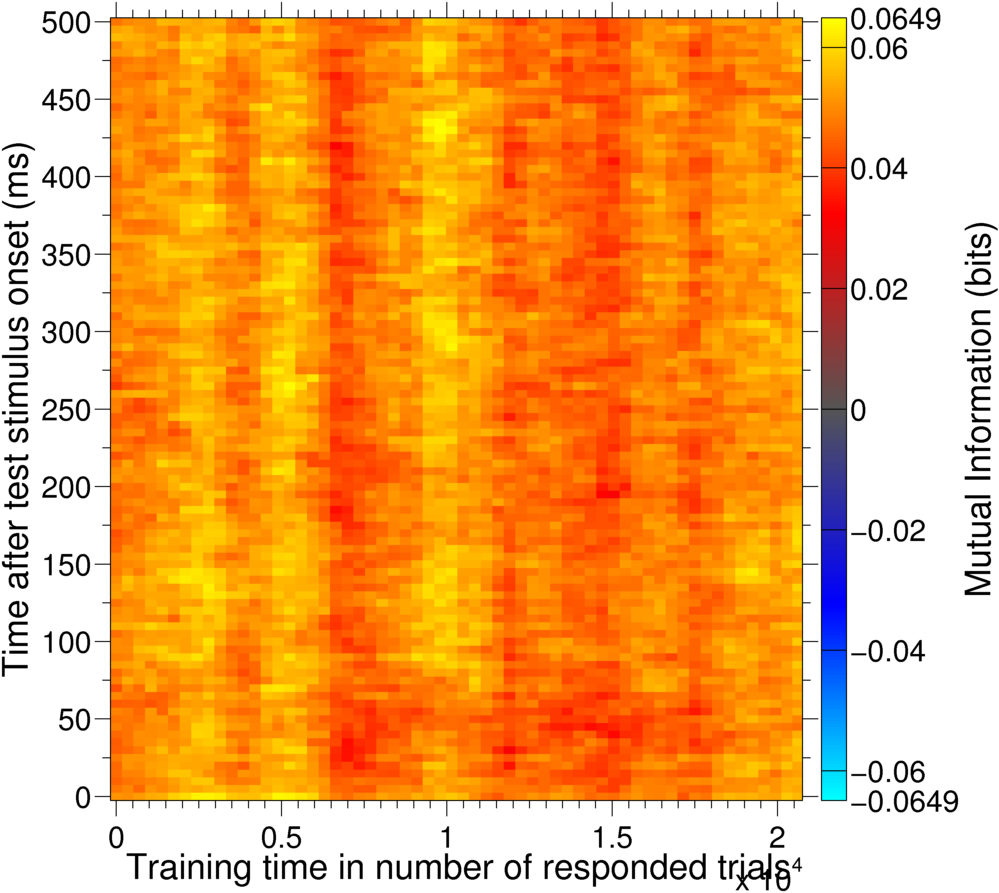
\includegraphics[scale=.25]{%
% % ./figs/I_trialwise_blanco_v4_chmean31_s307,308,311,313,314,317,318,320,321,329-341_tp1_5bins_of_4ms_dr_pt_oc0_test_tc10-5-25,27-29,31-33,35,40-10-60_nt1400_ts350_rmvet1_rmvms1_pcolorbp_20120816T175438.png}
% %     \end{subfigure}
% %     \caption{M1 V4: Mutual information between the test stimulus and \unit[20]{ms} of spiking activity, averaged across 30 channels.
% % The PT bias correction method was used in all estimates of the information.
% % Panels \ref{fig:b4-1x20tp4}--\ref{fig:b4-5x4tp1} are the same as for Fig.~\ref{fig:b1-trialwise}.
% % % The neural code used in \ref{fig:b4-1x20tp4ma}--\ref{fig:b4-1x20tp1} is a spike count code, whilst in \ref{fig:b4-5x4tp4}, \ref{fig:b4-5x4tp1} it is a spike timing code where the \unit[20]{ms} window was subdivided into 5 bins each of \unit[4]{ms}.
% % % In \ref{fig:b4-1x20tp4ma}, \ref{fig:b4-1x20tp4}, and \ref{fig:b4-5x4tp4}, the spike-train is taken from the test presentation part of the trial;
% % % for \ref{fig:b4-1x20tp1ma}, \ref{fig:b4-1x20tp1}, and \ref{fig:b4-5x4tp1}, the spike-train is taken from spontaneous pre-stimulus activity.
% % % In \ref{fig:b4-1x20tp4ma} and \ref{fig:b4-1x20tp1ma} no attempt was made to remove the monitor artifact from the raw data, whilst in the rest of the panels the data was modified to counter this as described in \ref{sec:ma}.
% % % \ref{fig:b4-1x20tp4ma}
% % % \ref{fig:b4-1x20tp1ma}
% % % \ref{fig:b4-1x20tp4}
% % % \ref{fig:b4-1x20tp1}
% % % \ref{fig:b4-5x4tp4}
% % % \ref{fig:b4-5x4tp1}
% % }
% %     \label{fig:b4-trialwise}
% % \end{figure}



% ./figs/I_trialwise_jack_v4_chmean20_s24-49_tp4_1bins_of_20ms_dr_pt_oc0_test_tc10-5-25,27-29,31-33,35,40-10-60_nt1400_ts350_rmvet1_rmvms0_pcolorhot_20120815T234433.png
% ./figs/I_trialwise_jack_v4_chmean20_s24-49_tp1_1bins_of_20ms_dr_pt_oc0_test_tc10-5-25,27-29,31-33,35,40-10-60_nt1400_ts350_rmvet1_rmvms1_pcolorbp_20120816T175433.png
% ./figs/I_trialwise_jack_v4_chmean20_s24-49_tp4_1bins_of_20ms_dr_pt_oc0_test_tc10-5-25,27-29,31-33,35,40-10-60_nt1400_ts350_rmvet1_rmvms1_pcolorhot_20120815T234723.png
% ./figs/I_trialwise_jack_v4_chmean20_s24-49_tp1_1bins_of_20ms_dr_pt_oc0_test_tc10-5-25,27-29,31-33,35,40-10-60_nt1400_ts350_rmvet1_rmvms1_pcolorhot_20120815T234559.png
% ./figs/I_trialwise_jack_v4_chmean20_s24-49_tp4_5bins_of_4ms_dr_pt_oc0_test_tc10-5-25,27-29,31-33,35,40-10-60_nt1400_ts350_rmvet1_rmvms1_pcolorhot_20120815T234455.png
% ./figs/I_trialwise_jack_v4_chmean20_s24-49_tp1_5bins_of_4ms_dr_pt_oc0_test_tc10-5-25,27-29,31-33,35,40-10-60_nt1400_ts350_rmvet1_rmvms1_pcolorbp_20120816T175404.png

% % \begin{figure}[htbp]
% % %     \begin{subfigure}[b]{0.5\linewidth}
% % %         \centering
% % %         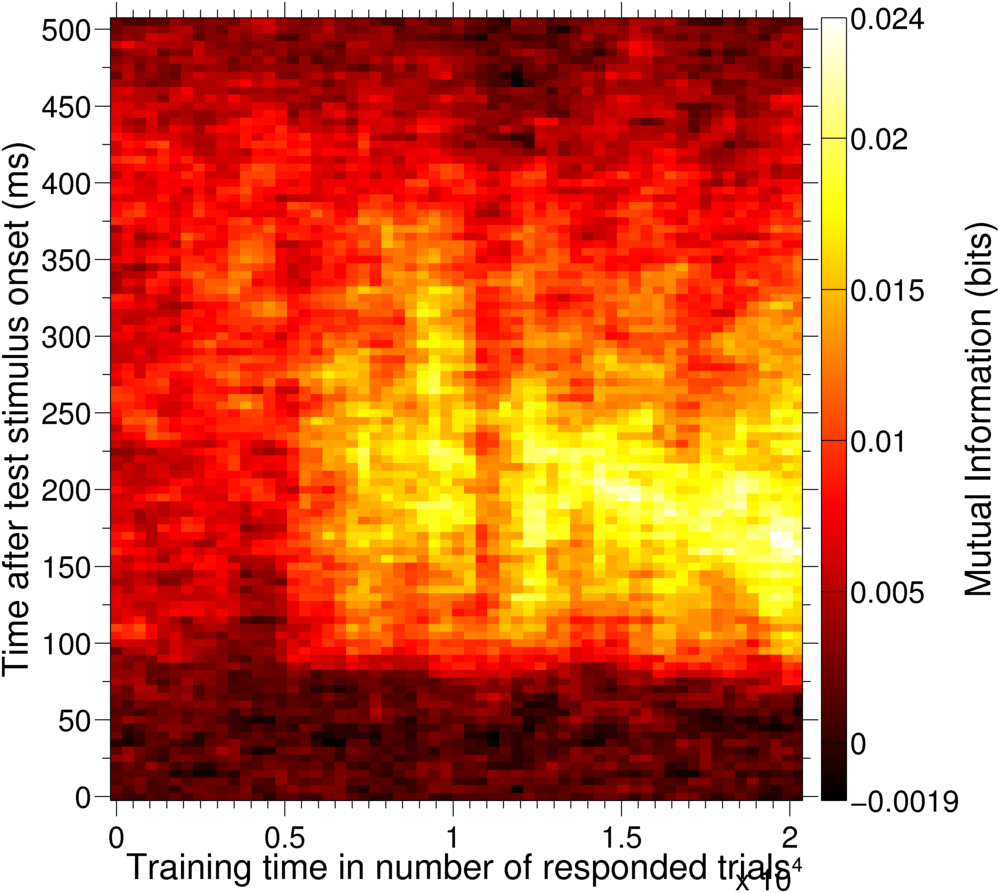
\includegraphics[scale=.25]{%
% % % ./figs/I_trialwise_jack_v4_chmean20_s24-49_tp4_1bins_of_20ms_dr_pt_oc0_test_tc10-5-25,27-29,31-33,35,40-10-60_nt1400_ts350_rmvet1_rmvms0_pcolorhot_20120815T234433.png}
% % %         \caption{}
% % %         \label{fig:j4-1x20tp4ma}
% % %     \end{subfigure}
% % %     ~~
% % %     \begin{subfigure}[b]{0.5\linewidth}
% % %         \centering
% % %         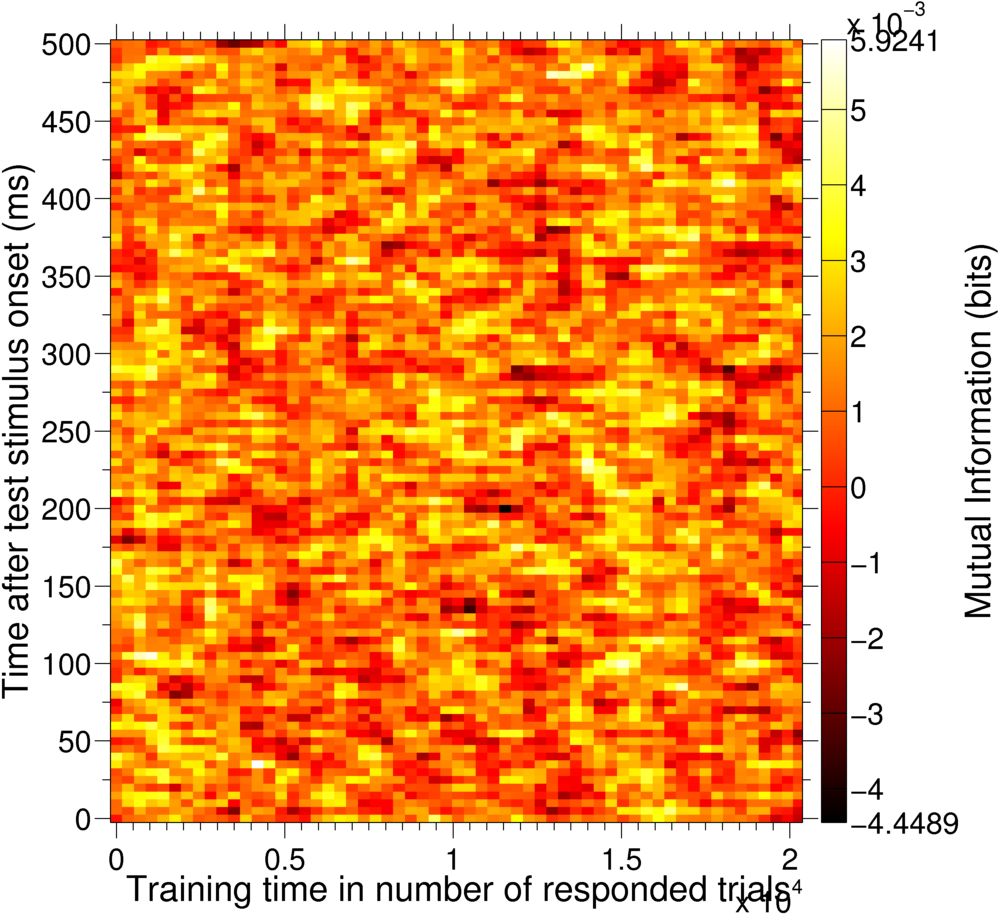
\includegraphics[scale=.25]{%
% % % ./figs/I_trialwise_jack_v4_chmean20_s24-49_tp1_1bins_of_20ms_dr_pt_oc0_test_tc10-5-25,27-29,31-33,35,40-10-60_nt1400_ts350_rmvet1_rmvms0_pcolorhot_20120815T234307.png}
% % %         \caption{}
% % %         \label{fig:j4-1x20tp1ma}
% % %     \end{subfigure}
% % %     \\
% %     \begin{subfigure}[b]{0.5\linewidth}
% %         \centering
% %         \caption{}
% %         \label{fig:j4-1x20tp4}
% %         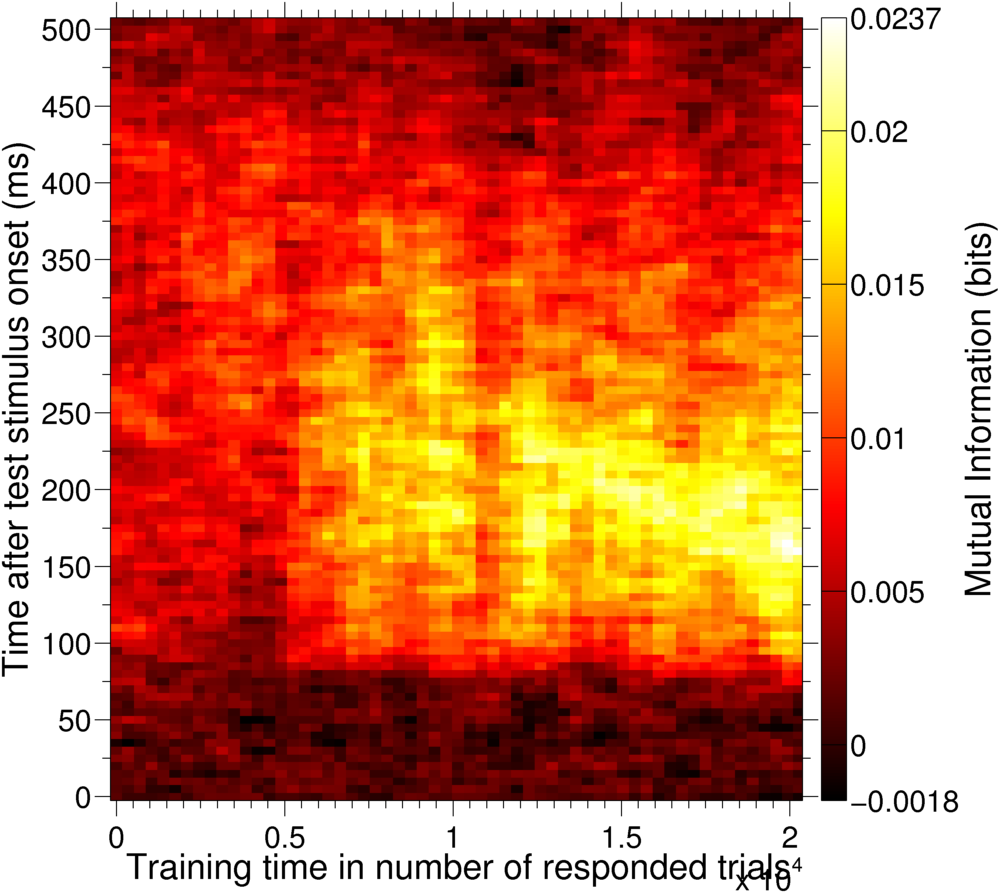
\includegraphics[scale=.25]{%
% % ./figs/I_trialwise_jack_v4_chmean20_s24-49_tp4_1bins_of_20ms_dr_pt_oc0_test_tc10-5-25,27-29,31-33,35,40-10-60_nt1400_ts350_rmvet1_rmvms1_pcolorhot_20120815T234723.png}
% %     \end{subfigure}
% %     ~~
% %     \begin{subfigure}[b]{0.5\linewidth}
% %         \centering
% %         \caption{}
% %         \label{fig:j4-1x20tp1}
% %         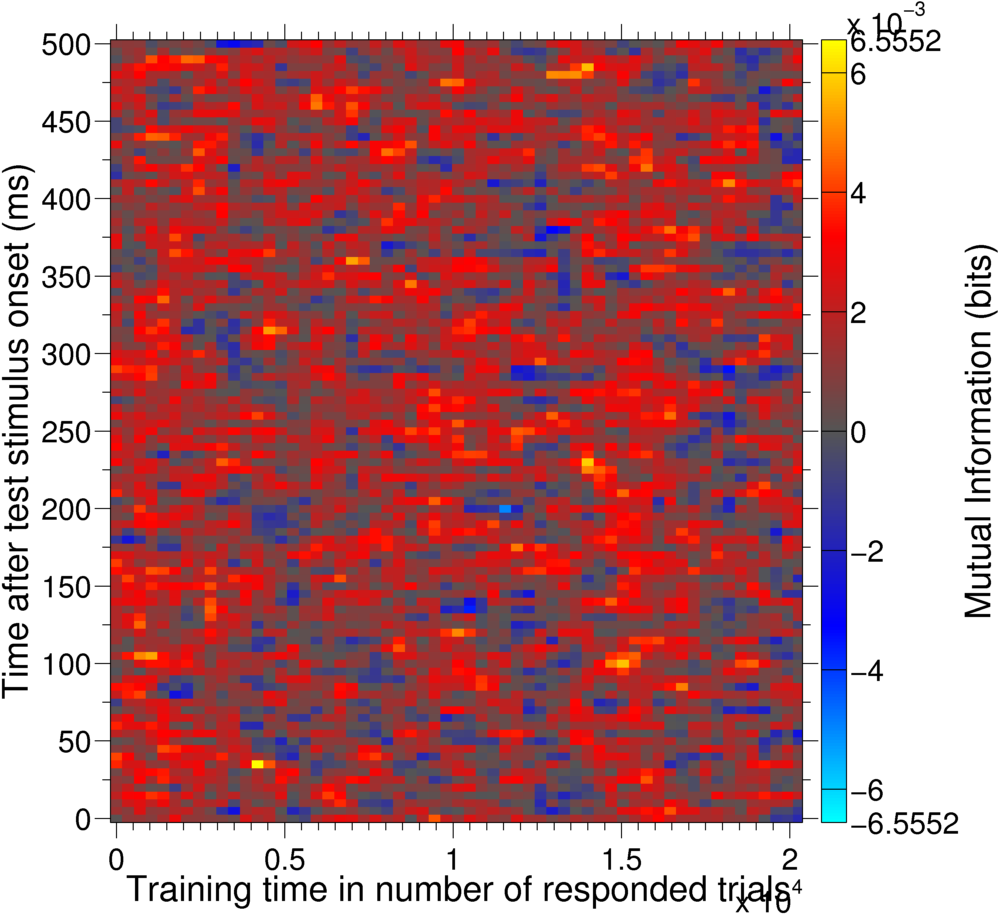
\includegraphics[scale=.25]{%
% % ./figs/I_trialwise_jack_v4_chmean20_s24-49_tp1_1bins_of_20ms_dr_pt_oc0_test_tc10-5-25,27-29,31-33,35,40-10-60_nt1400_ts350_rmvet1_rmvms1_pcolorbp_20120816T175433.png}
% %     \end{subfigure}
% %     \\
% %     \begin{subfigure}[b]{0.5\linewidth}
% %         \centering
% %         \caption{}
% %         \label{fig:j4-5x4tp4}
% %         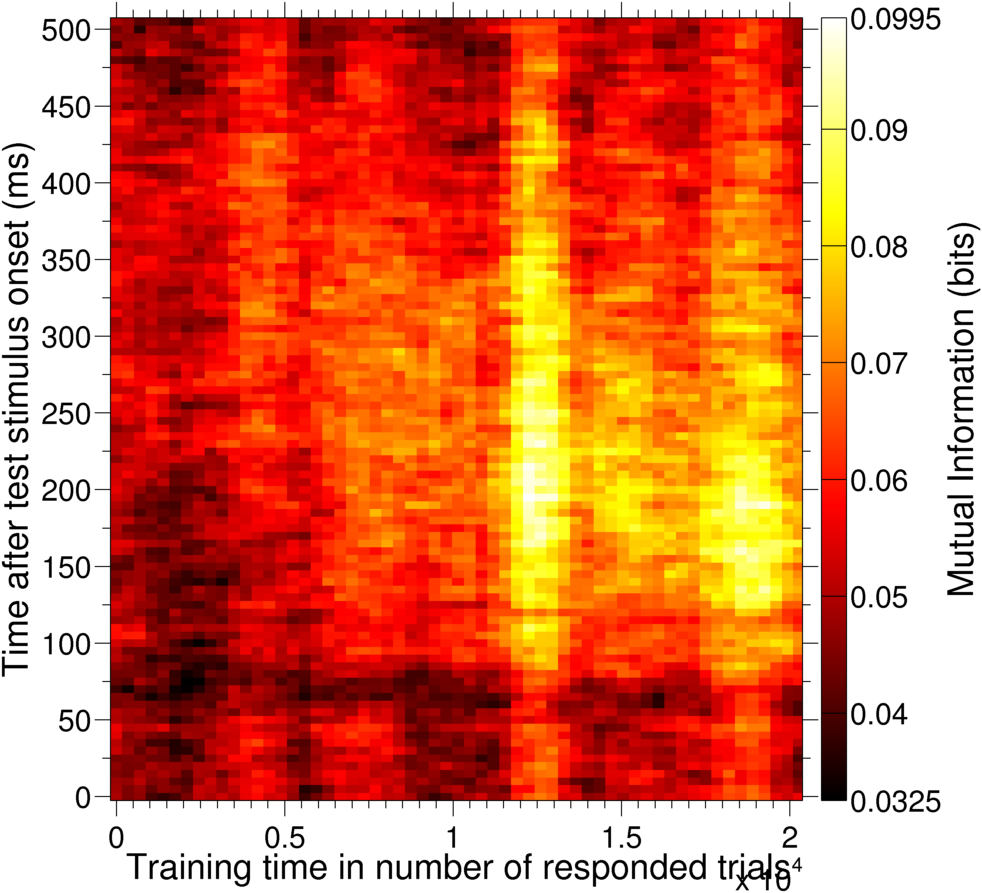
\includegraphics[scale=.25]{%
% % ./figs/I_trialwise_jack_v4_chmean20_s24-49_tp4_5bins_of_4ms_dr_pt_oc0_test_tc10-5-25,27-29,31-33,35,40-10-60_nt1400_ts350_rmvet1_rmvms1_pcolorhot_20120815T234455.png}
% %     \end{subfigure}
% %     ~~
% %     \begin{subfigure}[b]{0.5\linewidth}
% %         \centering
% %         \caption{}
% %         \label{fig:j4-5x4tp1}
% %         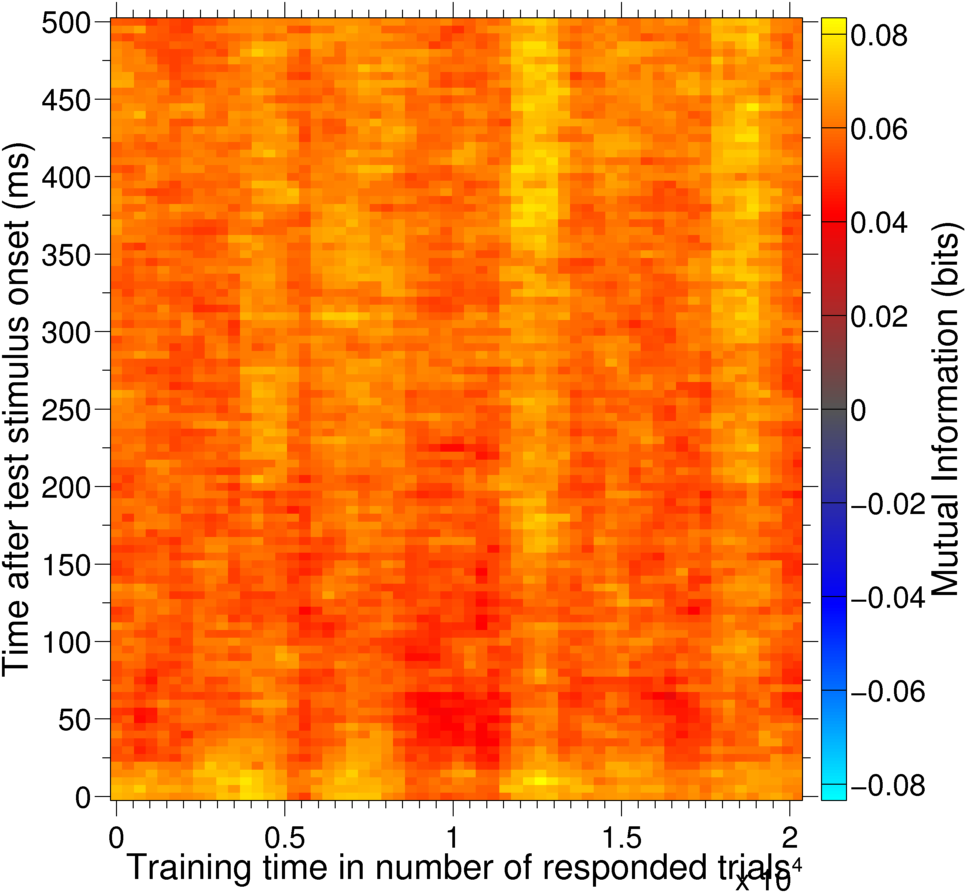
\includegraphics[scale=.25]{%
% % ./figs/I_trialwise_jack_v4_chmean20_s24-49_tp1_5bins_of_4ms_dr_pt_oc0_test_tc10-5-25,27-29,31-33,35,40-10-60_nt1400_ts350_rmvet1_rmvms1_pcolorbp_20120816T175404.png}
% %     \end{subfigure}
% %     \caption{M2 V4: Mutual information between the test stimulus and \unit[20]{ms} of spiking activity, averaged across 20 channels.
% % The PT bias correction method was used in all estimates of the information.
% % Panels \ref{fig:j4-1x20tp4}--\ref{fig:j4-5x4tp1} are the same as for Fig.~\ref{fig:b1-trialwise}.
% % % The neural code used in \ref{fig:j4-1x20tp4ma}--\ref{fig:j4-1x20tp1} is a spike count code, whilst in \ref{fig:j4-5x4tp4}, \ref{fig:j4-5x4tp1} it is a spike timing code where the \unit[20]{ms} window was subdivided into 5 bins each of \unit[4]{ms}.
% % % In \ref{fig:j4-1x20tp4ma}, \ref{fig:j4-1x20tp4}, and \ref{fig:j4-5x4tp4}, the spike-train is taken from the test presentation part of the trial;
% % % for \ref{fig:j4-1x20tp1ma}, \ref{fig:j4-1x20tp1}, and \ref{fig:j4-5x4tp1}, the spike-train is taken from spontaneous pre-stimulus activity.
% % % In \ref{fig:j4-1x20tp4ma} and \ref{fig:j4-1x20tp1ma} no attempt was made to remove the monitor artifact from the raw data, whilst in the rest of the panels the data was modified to counter this as described in \ref{sec:ma}.
% % % \ref{fig:j4-1x20tp4ma}
% % % \ref{fig:j4-1x20tp1ma}
% % % \ref{fig:j4-1x20tp4}
% % % \ref{fig:j4-1x20tp1}
% % % \ref{fig:j4-5x4tp4}
% % % \ref{fig:j4-5x4tp1}
% % }
% %     \label{fig:j4-trialwise}
% % \end{figure}

% 20, 30 and \unit[40]{ms} all tried. Mutual information increases as the duration increases as one would expect, but there is no other significant difference. Consequently only 20ms is shown in this section.

% More information with only correct trials used, but this could be due to differences in $P(S)$.

Turning our attention to the V4 results in Figs.~\ref{fig:b4-trialwise} and \ref{fig:j4-trialwise}, we can see the effect of the transient is present in M1's data (at the later start time of \unit[75]{ms}), but not in M2's. This is surprising because, looking at the rasters, in both animals there are some channels which exhibit a transient response and some which do not.

Similar to V1, it seems as if there is four times as much information in the timebinned code compared with the count code. However, there is much more information measured for the spontaneous activity data again. This is not reduced by increasing the number of trials either.

For the spike count code in M2, the spontaneous information is nearly distributed around 0, suggesting the bias has been all but removed and the data is of very high quality. For this animal, we can see a distinct increase in the information content with time, for both the spike count and timing codes. Simultaneously, there is a movement of the peak information to earlier times closer to the stimulus onset.

In M1, there is a small increase in the information content with time which may or may not significant. However, it is reassuring to see that this is not due to an improvement in the data with time, as the trend in the spontaneous activity information bias (Fig.~\ref{fig:j4-5x4tp1}) is a decrease with time.

%----------------------------------------------------------------------------------------------------------------------
\FloatBarrier
\subsubsection{Fine vs coarse contrast differences}

Comparing Figs.~\ref{fig:b1-1x20cc} and \ref{fig:j1-1x20cc} where the outer 6 contrasts are included with Figs.~\ref{fig:b1-1x20tp4} and \ref{fig:b1-1x20tp4} where all contrasts are included, it seems as if the amount of information has increased, which should not be possible. However, the difference will be due to the difference in trials contained in each of the analyses. In each case, an average of 100 trials per stimulus is used, but since the easier test conditions are presented less frequently, they are under-represented in Figs.~\ref{fig:b1-1x20tp4} and \ref{fig:b1-1x20tp4} (about 75 trials per stimulus). Obviously these are more discriminable, so the under-representation comparably reduces the information.

Looking at V1 (Fig.~\ref{fig:v1-fvc}), we observe there is much more information for M2 than M1, as we found before. The quality of the data seems to have severely hampered the analysis for M1, destroying the the fine differences in the data needed to evaluate the information contained about fine contrast differences (Fig.~\ref{fig:b1-1x20fc}).

Unsurprisingly, there is more information when considering the coarsely distinct contrasts than the finer differences, as the neural activity is bound to be more discriminable for these. For M2, there is a small upward trend again for both coarse and fine contrast differences, which may or may not be genuine.

% ./figs/I_trialwise_blanco_v1_chmean23_s343-354,355.1,355.2,356-359_tp4_1bins_of_20ms_dr_pt_oc0_test_tc5,15,22,40,50,90_nt600_ts150_rmvet1_rmvms1_pcolorhot_20120816T011936.png
% ./figs/I_trialwise_blanco_v1_chmean23_s343-354,355.1,355.2,356-359_tp4_1bins_of_20ms_dr_pt_oc0_test_tc22-3-28,32,35,40_nt600_ts150_rmvet1_rmvms1_pcolorhot_20120816T011920.png
% ./figs/I_trialwise_jack_v1_chmean25_s51-72_tp4_1bins_of_20ms_dr_pt_oc0_test_tc5,15,22,40,50,90_nt600_ts150_rmvet1_rmvms1_pcolorhot_20120816T011822.png
% ./figs/I_trialwise_jack_v1_chmean25_s51-72_tp4_1bins_of_20ms_dr_pt_oc0_test_tc22-3-28,32,35,40_nt600_ts150_rmvet1_rmvms1_pcolorhot_20120816T011800.png

% % \begin{figure}[htbp]
% %     \begin{subfigure}[b]{0.5\linewidth}
% %         \centering
% %         \caption{}
% %         \label{fig:b1-1x20cc}
% %         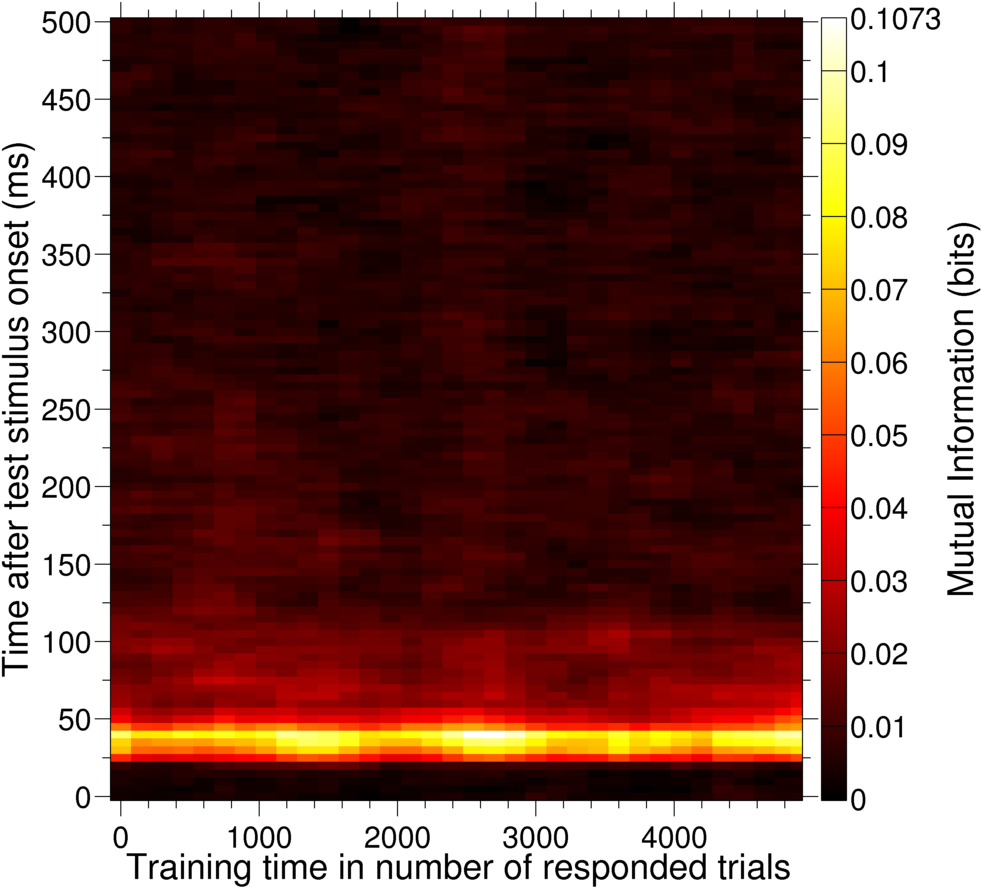
\includegraphics[scale=.25]{%
% % ./figs/I_trialwise_blanco_v1_chmean23_s343-354,355.1,355.2,356-359_tp4_1bins_of_20ms_dr_pt_oc0_test_tc5,15,22,40,50,90_nt600_ts150_rmvet1_rmvms1_pcolorhot_20120816T011936.png}
% %     \end{subfigure}
% %     ~~
% %     \begin{subfigure}[b]{0.5\linewidth}
% %         \centering
% %         \caption{}
% %         \label{fig:j1-1x20cc}
% %         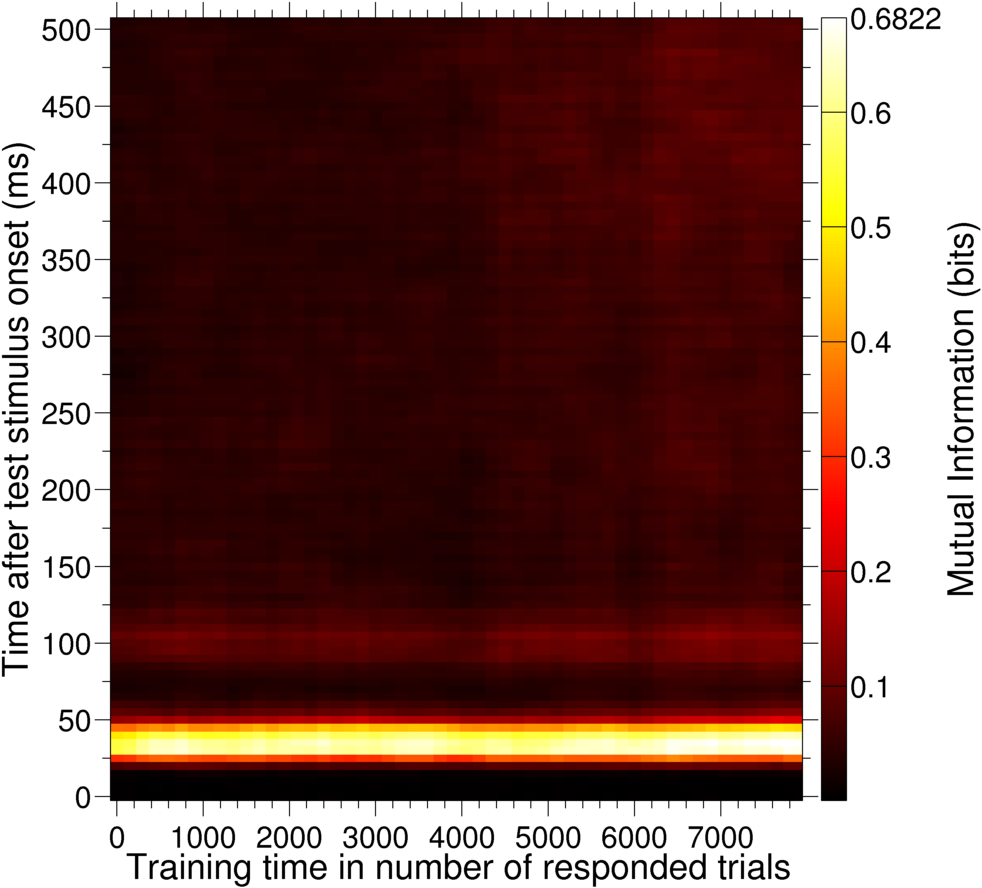
\includegraphics[scale=.25]{%
% % ./figs/I_trialwise_jack_v1_chmean25_s51-72_tp4_1bins_of_20ms_dr_pt_oc0_test_tc5,15,22,40,50,90_nt600_ts150_rmvet1_rmvms1_pcolorhot_20120816T011822.png}
% %     \end{subfigure}
% %     \\
% %     \begin{subfigure}[b]{0.5\linewidth}
% %         \centering
% %         \caption{}
% %         \label{fig:b1-1x20fc}
% %         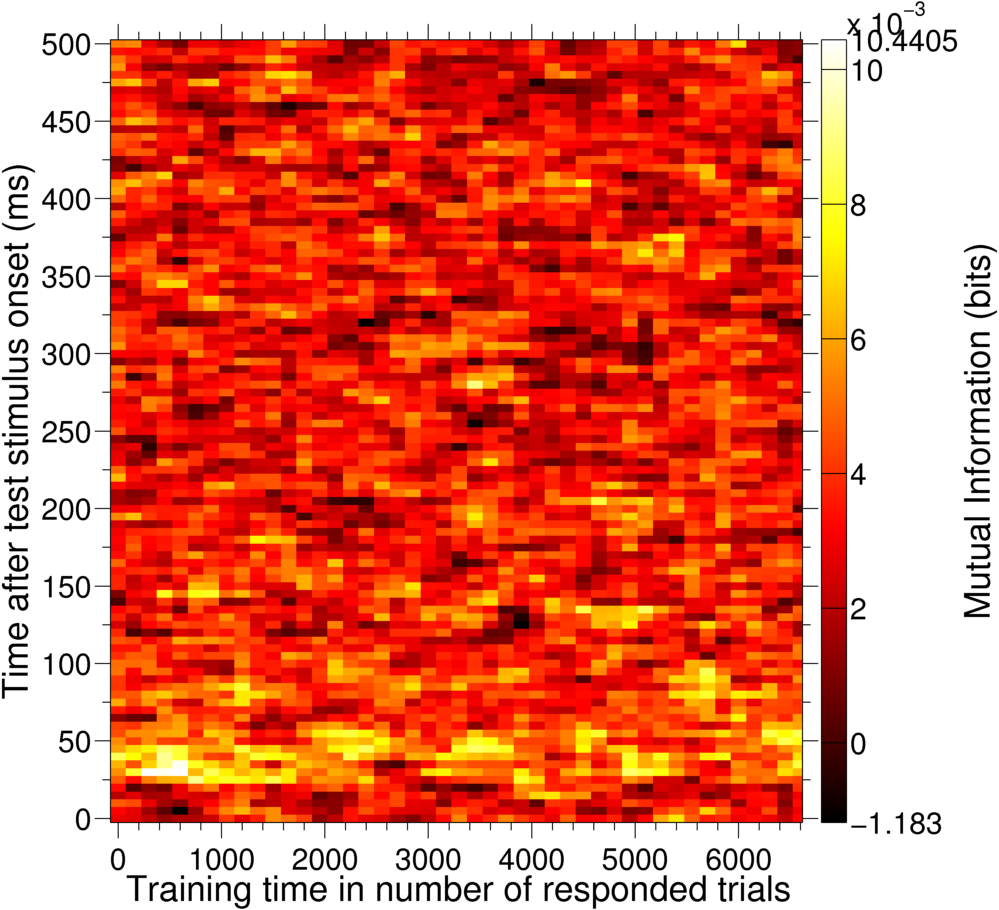
\includegraphics[scale=.25]{%
% % ./figs/I_trialwise_blanco_v1_chmean23_s343-354,355.1,355.2,356-359_tp4_1bins_of_20ms_dr_pt_oc0_test_tc22-3-28,32,35,40_nt600_ts150_rmvet1_rmvms1_pcolorhot_20120816T011920.png}
% %     \end{subfigure}
% %     ~~
% %     \begin{subfigure}[b]{0.5\linewidth}
% %         \centering
% %         \caption{}
% %         \label{fig:j1-1x20fc}
% %         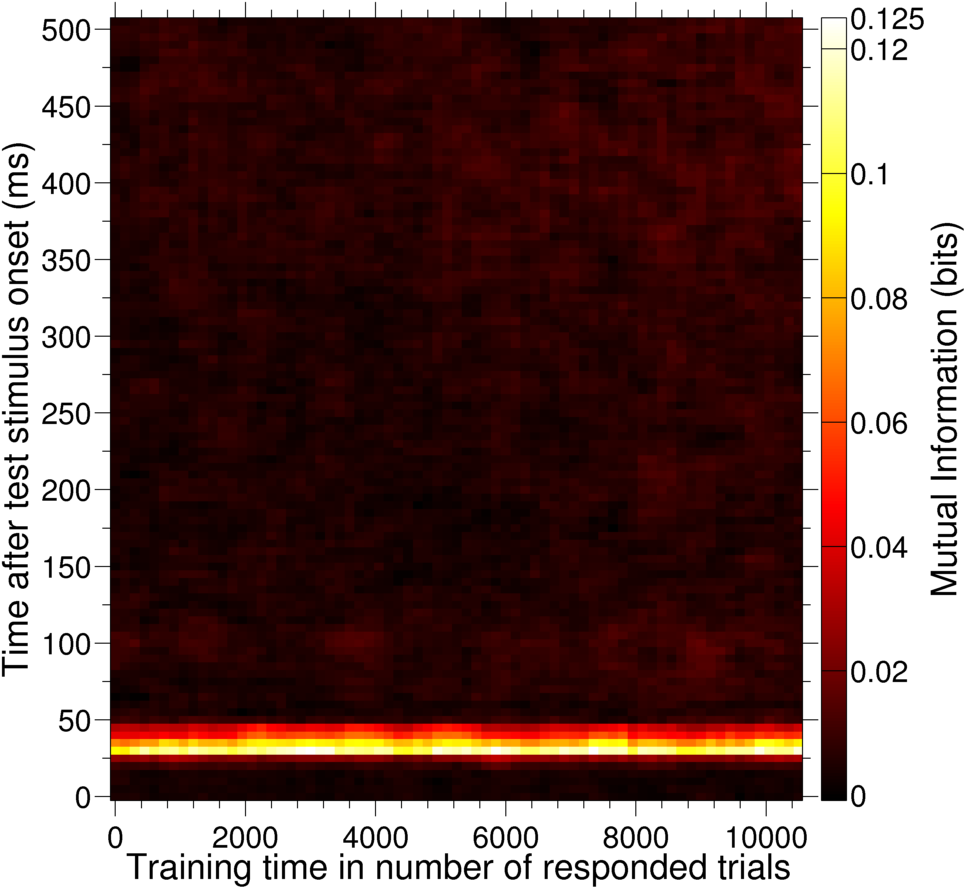
\includegraphics[scale=.25]{%
% % ./figs/I_trialwise_jack_v1_chmean25_s51-72_tp4_1bins_of_20ms_dr_pt_oc0_test_tc22-3-28,32,35,40_nt600_ts150_rmvet1_rmvms1_pcolorhot_20120816T011800.png}
% %     \end{subfigure}
% %     \caption{V1: Fine vs. coarse contrast differences.
% % % Mutual information between the test stimulus and \unit[20]{ms} of spiking activity.
% % % The PT bias correction method was used in all estimates of the information.
% % In the top panels, the six contrasts included are \{5, 15, 22, 40, 50, 90\}\%; bottom panels \{22, 25, 28, 32, 35, 40\}\%. An average of 100 trials per stimulus is used in each of these.
% % Left panels are for M1, right are M2.
% % In each case, mutual information between the six test stimuli and \unit[20]{ms} of spiking activity was measured using a spike count code, and bias corrected using the PT method.
% % % Panels \ref{fig:b1-1x20cc} and \ref{fig:b1-1x20fc} are for M1, \ref{fig:b1-1x20cc} and \ref{fig:b1-1x20fc} for M2.
% % }
% %     \label{fig:v1-fvc}
% % \end{figure}


% ./figs/I_trialwise_blanco_v4_chmean31_s307,308,311,313,314,317,318,320,321,329-341_tp4_1bins_of_20ms_dr_pt_oc0_test_tc10-5-20,40-10-60_nt600_ts150_rmvet1_rmvms1_pcolorhot_20120816T012120.png
% ./figs/I_trialwise_blanco_v4_chmean31_s307,308,311,313,314,317,318,320,321,329-341_tp4_1bins_of_20ms_dr_pt_oc0_test_tc27-29,31-33_nt600_ts150_rmvet1_rmvms1_pcolorhot_20120816T011952.png
% ./figs/I_trialwise_jack_v4_chmean20_s24-49_tp4_1bins_of_20ms_dr_pt_oc0_test_tc10-5-20,40-10-60_nt600_ts150_rmvet1_rmvms1_pcolorhot_20120816T011902.png
% ./figs/I_trialwise_jack_v4_chmean20_s24-49_tp4_1bins_of_20ms_dr_pt_oc0_test_tc27-29,31-33_nt600_ts150_rmvet1_rmvms1_pcolorhot_20120816T011843.png

% % \begin{figure}[htbp]
% %     \begin{subfigure}[b]{0.5\linewidth}
% %         \centering
% %         \caption{}
% %         \label{fig:b4-1x20cc}
% %         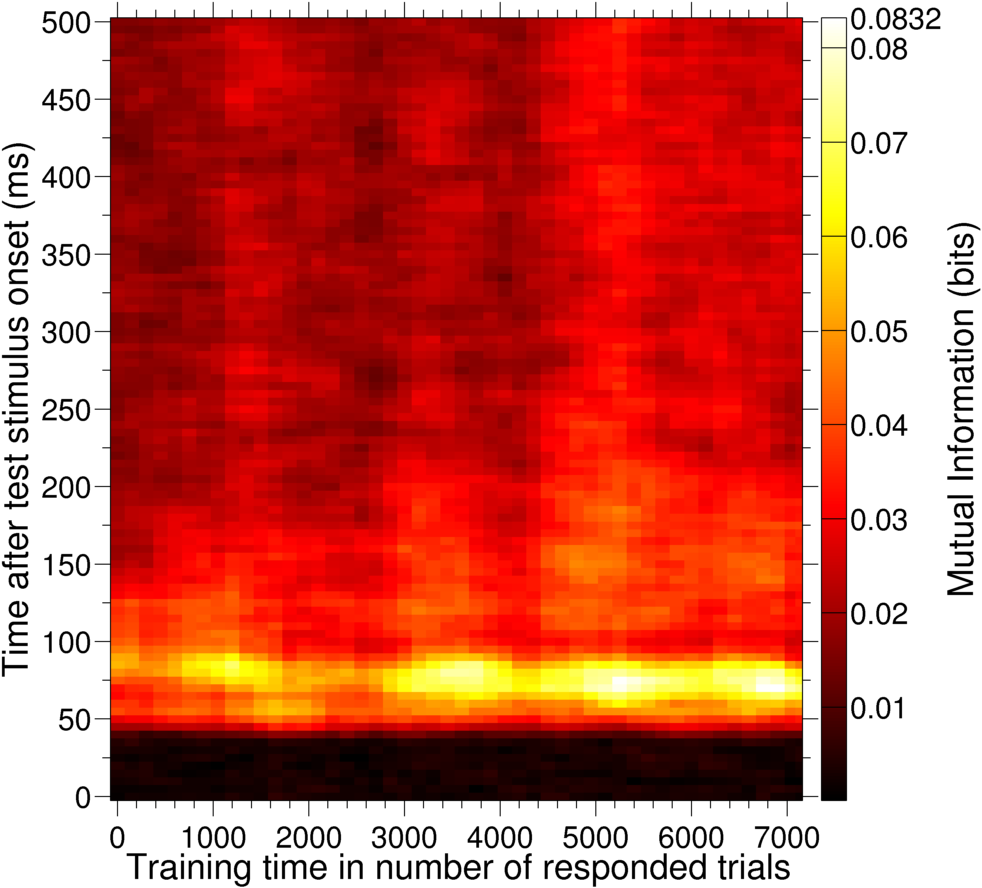
\includegraphics[scale=.25]{%
% % ./figs/I_trialwise_blanco_v4_chmean31_s307,308,311,313,314,317,318,320,321,329-341_tp4_1bins_of_20ms_dr_pt_oc0_test_tc10-5-20,40-10-60_nt600_ts150_rmvet1_rmvms1_pcolorhot_20120816T012120.png}
% %     \end{subfigure}
% %     ~~
% %     \begin{subfigure}[b]{0.5\linewidth}
% %         \centering
% %         \caption{}
% %         \label{fig:j4-1x20cc}
% %         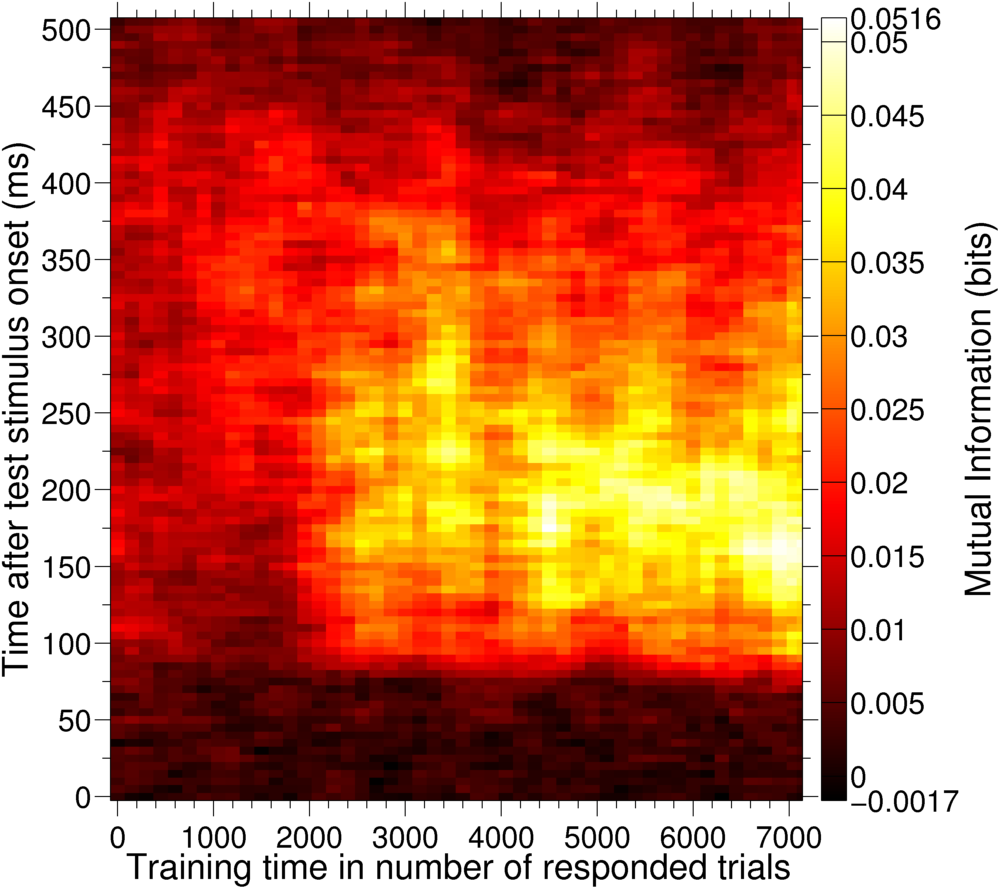
\includegraphics[scale=.25]{%
% % ./figs/I_trialwise_jack_v4_chmean20_s24-49_tp4_1bins_of_20ms_dr_pt_oc0_test_tc10-5-20,40-10-60_nt600_ts150_rmvet1_rmvms1_pcolorhot_20120816T011902.png}
% %     \end{subfigure}
% %     \\
% %     \begin{subfigure}[b]{0.5\linewidth}
% %         \centering
% %         \caption{}
% %         \label{fig:b4-1x20fc}
% %         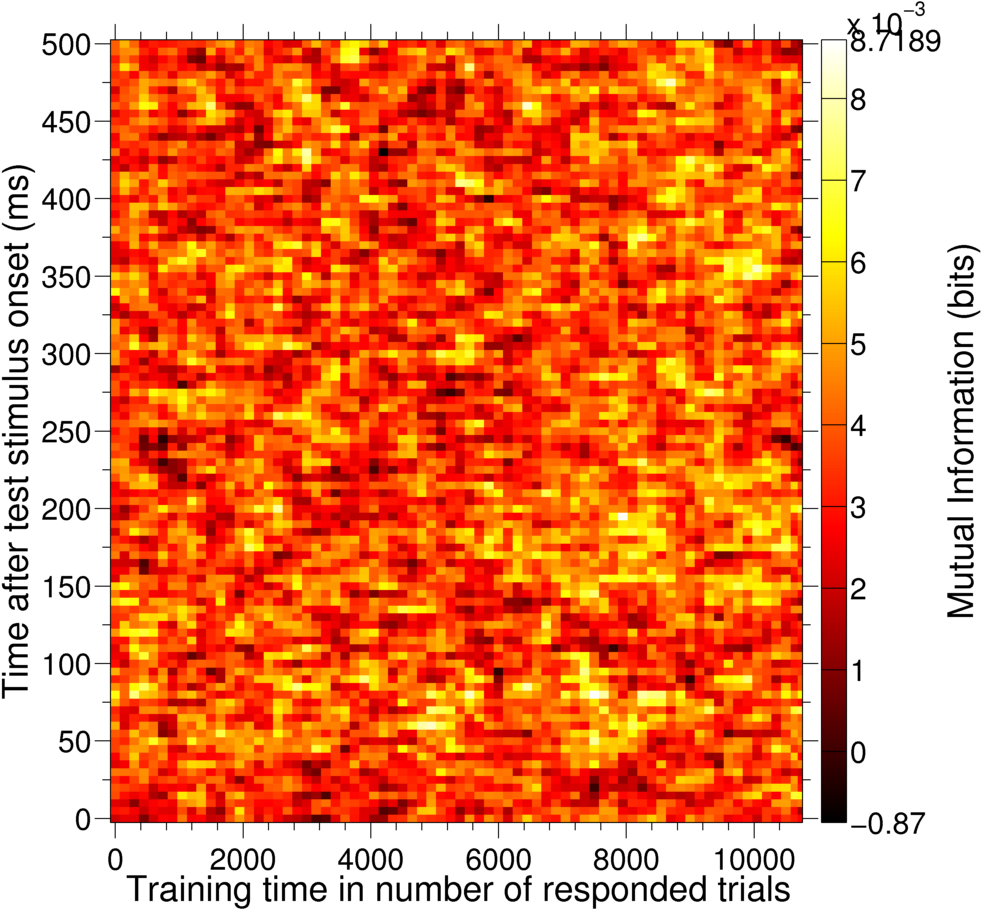
\includegraphics[scale=.25]{%
% % ./figs/I_trialwise_blanco_v4_chmean31_s307,308,311,313,314,317,318,320,321,329-341_tp4_1bins_of_20ms_dr_pt_oc0_test_tc27-29,31-33_nt600_ts150_rmvet1_rmvms1_pcolorhot_20120816T011952.png}
% %     \end{subfigure}
% %     ~~
% %     \begin{subfigure}[b]{0.5\linewidth}
% %         \centering
% %         \caption{}
% %         \label{fig:j4-1x20fc}
% %         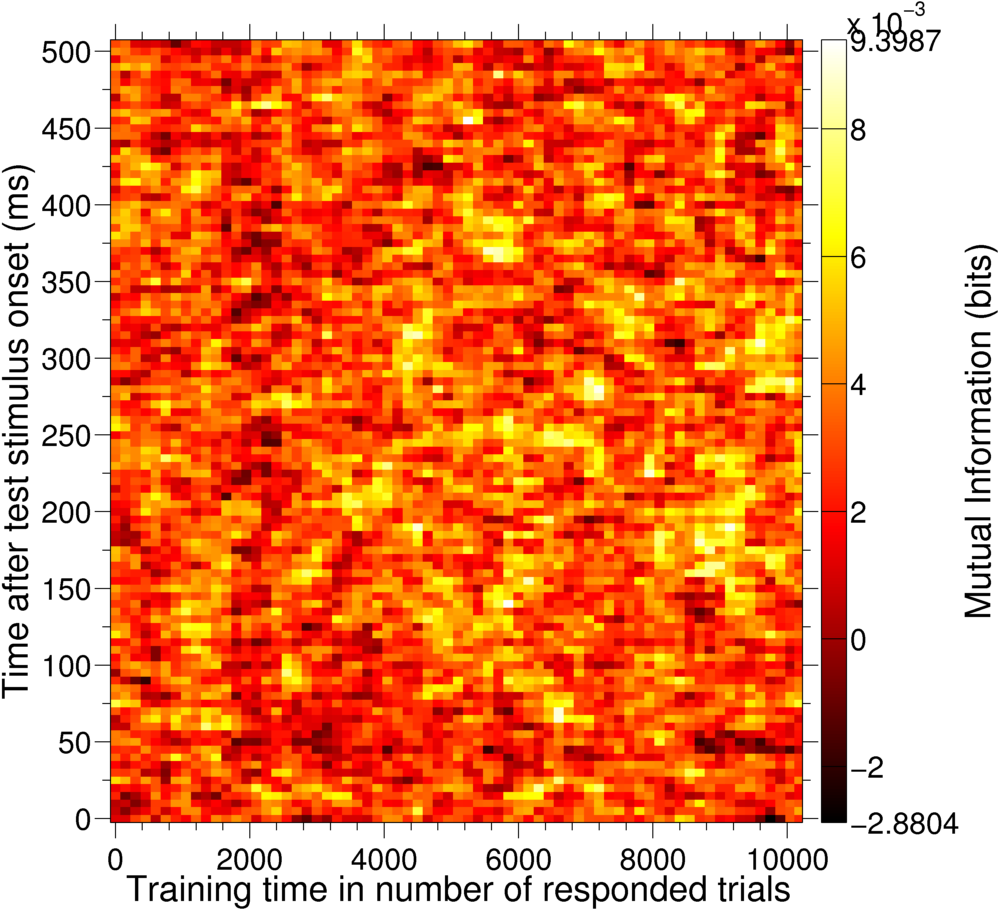
\includegraphics[scale=.25]{%
% % ./figs/I_trialwise_jack_v4_chmean20_s24-49_tp4_1bins_of_20ms_dr_pt_oc0_test_tc27-29,31-33_nt600_ts150_rmvet1_rmvms1_pcolorhot_20120816T011843.png}
% %     \end{subfigure}
% %     \caption{V4: Fine vs coarse contrast differences.
% % % Mutual information between the test stimulus and \unit[20]{ms} of spiking activity.
% % % The PT bias correction method was used in all estimates of the information.
% % In the top panels, the six contrasts included are \{10, 15, 20, 40, 50, 60\}\%; bottom panels \{27, 28, 29, 31, 32, 33\}\%. An average of 100 trials per stimulus is used in each of these.
% % Left panels are for M1, right are M2.
% % In each case, mutual information between the six test stimuli and \unit[20]{ms} of spiking activity was measured using a spike count code, and bias corrected using the PT method.
% % % Panels \ref{fig:b1-1x20cc} and \ref{fig:b1-1x20fc} are for M1, \ref{fig:b1-1x20cc} and \ref{fig:b1-1x20fc} for M2.
% % }
% %     \label{fig:v4-fvc}
% % \end{figure}

For V4, we find there is no information about fine contrast differences in either animal (Figs.~\ref{fig:b4-1x20fc} and \ref{fig:j4-1x20fc}). The information about the coarse differences is higher than when all conditions are considered, for reasons discussed above, and these show the same trends as when we analysed all the conditions, in Figs.~\ref{fig:b4-1x20tp4} and \ref{fig:j4-1x20tp4}.

%----------------------------------------------------------------------------------------------------------------------
\FloatBarrier
\subsubsection{Information in millisecond-level spike timing}

For M2 V1, there seems to be some information in the millisecond-level timing of the spikes during the transient response, but not afterward this has elapsed (Fig.~\ref{fig:v1-dif}, right-hand panels). This band due to the transient is clearly well above the variance of the sampling for the rest of the window offsets.
However, the information in the transient is only present for the coarse contrasts and not for the fine contrasts.
For the fine contrast discrimination in M2 V1, shown in Fig.~\ref{fig:j1-fdif}, (and possibly to a lesser degree on a couple of the other figures) there is an unusual effect where there seems to be more information in the shuffled bins than the unshuffled bins.\footnote{When this is analysed for the raw data with the artifact included, this is subtly more prominently on several of the plots.}

For M1 V1, and also M1 V4, there seems to be an increase in the information contained in the spike timing during the transient also. However, these results are not as clear-cut as in M2 V1.

% ./figs/I_diff_trialwise_dur=20ms_nshuf=1_blanco_v1_chmean23_s343-354,355.1,355.2,356-359_tp4_dr_pt_oc0_test_tc5-5-20,22-3-28,32,35-5-50,60,90_nt1400_ts350_rmvet1_rmvms1_pcolorbp_20120816T010538.png
% ./figs/I_diff_trialwise_dur=20ms_nshuf=1_blanco_v1_chmean23_s343-354,355.1,355.2,356-359_tp4_dr_pt_oc0_test_tc5,15,22,40,50,90_nt600_ts150_rmvet1_rmvms1_pcolorbp_20120816T004933.png
% ./figs/I_diff_trialwise_dur=20ms_nshuf=1_blanco_v1_chmean23_s343-354,355.1,355.2,356-359_tp4_dr_pt_oc0_test_tc22-3-28,32,35,40_nt600_ts150_rmvet1_rmvms1_pcolorbp_20120816T004908.png
% 
% ./figs/I_diff_trialwise_dur=20ms_nshuf=1_jack_v1_chmean25_s51-72_tp4_dr_pt_oc0_test_tc5-5-20,22-3-28,32,35-5-50,60,90_nt1400_ts350_rmvet1_rmvms1_pcolorbp_20120816T004517.png
% ./figs/I_diff_trialwise_dur=20ms_nshuf=1_jack_v1_chmean25_s51-72_tp4_dr_pt_oc0_test_tc5,15,22,40,50,90_nt600_ts150_rmvet1_rmvms1_pcolorbp_20120816T010526.png
% ./figs/I_diff_trialwise_dur=20ms_nshuf=1_jack_v1_chmean25_s51-72_tp4_dr_pt_oc0_test_tc22-3-28,32,35,40_nt600_ts150_rmvet1_rmvms1_pcolorbp_20120816T004555.png

% % \begin{figure}[htbp]
% %     \begin{subfigure}[b]{0.5\linewidth}
% %         \centering
% %         \caption{}
% %         \label{fig:b1-alldif}
% %         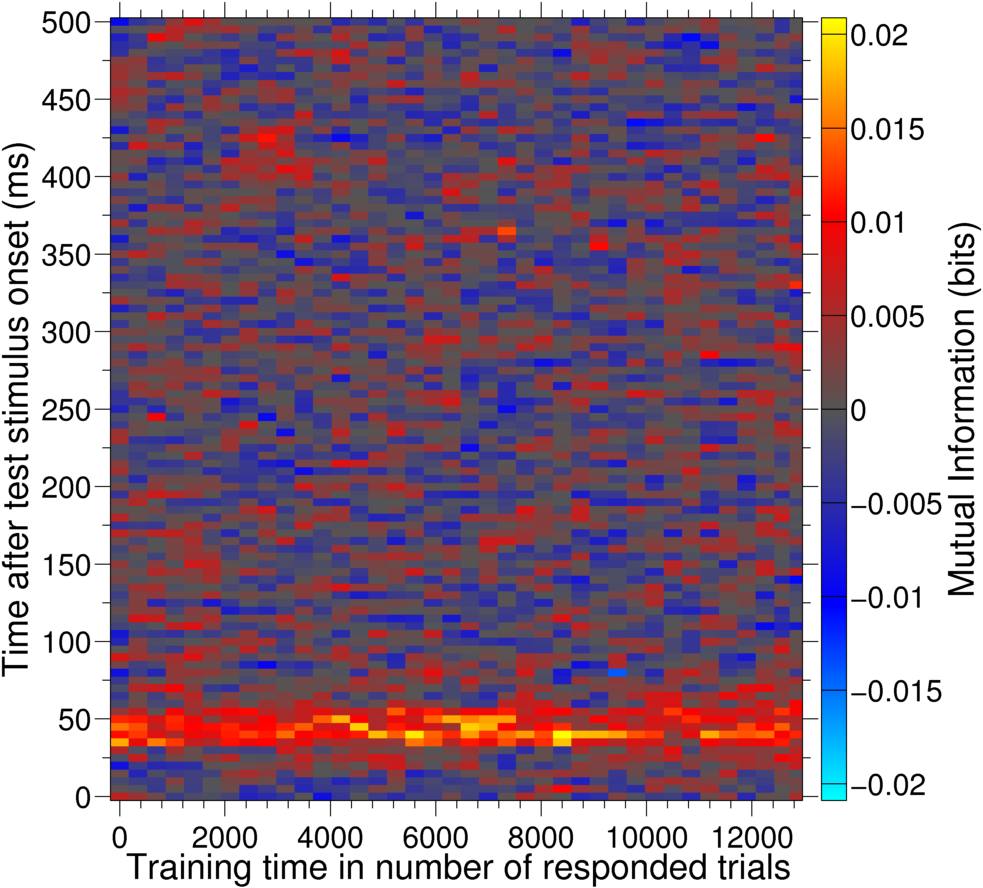
\includegraphics[scale=.25]{%
% % ./figs/I_diff_trialwise_dur=20ms_nshuf=1_blanco_v1_chmean23_s343-354,355.1,355.2,356-359_tp4_dr_pt_oc0_test_tc5-5-20,22-3-28,32,35-5-50,60,90_nt1400_ts350_rmvet1_rmvms1_pcolorbp_20120816T010538.png}
% %     \end{subfigure}
% %     ~~
% %     \begin{subfigure}[b]{0.5\linewidth}
% %         \centering
% %         \caption{}
% %         \label{fig:j1-alldif}
% %         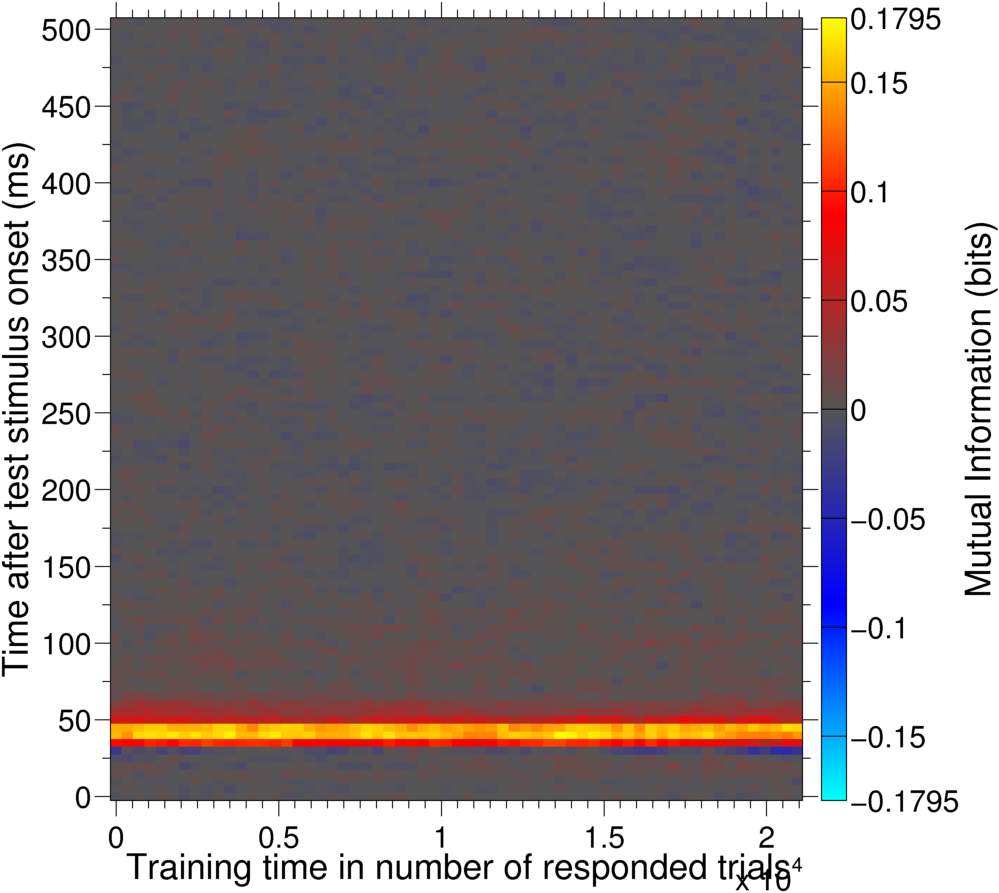
\includegraphics[scale=.25]{%
% % ./figs/I_diff_trialwise_dur=20ms_nshuf=1_jack_v1_chmean25_s51-72_tp4_dr_pt_oc0_test_tc5-5-20,22-3-28,32,35-5-50,60,90_nt1400_ts350_rmvet1_rmvms1_pcolorbp_20120816T004517.png}
% %     \end{subfigure}
% %     \\
% %     \begin{subfigure}[b]{0.5\linewidth}
% %         \centering
% %         \caption{}
% %         \label{fig:b1-cdif}
% %         \includegraphics[scale=.25]{%
% % ./figs/I_diff_trialwise_dur=20ms_nshuf=1_blanco_v1_chmean23_s343-354,355.1,355.2,356-359_tp4_dr_pt_oc0_test_tc5,15,22,40,50,90_nt600_ts150_rmvet1_rmvms1_pcolorbp_20120816T004933.png}
% %     \end{subfigure}
% %     ~~
% %     \begin{subfigure}[b]{0.5\linewidth}
% %         \centering
% %         \caption{}
% %         \label{fig:j1-cdif}
% %         \includegraphics[scale=.25]{%
% % ./figs/I_diff_trialwise_dur=20ms_nshuf=1_jack_v1_chmean25_s51-72_tp4_dr_pt_oc0_test_tc5,15,22,40,50,90_nt600_ts150_rmvet1_rmvms1_pcolorbp_20120816T010526.png}
% %     \end{subfigure}
% %     \\
% %     \begin{subfigure}[b]{0.5\linewidth}
% %         \centering
% %         \caption{}
% %         \label{fig:b1-fdif}
% %         \includegraphics[scale=.25]{%
% % ./figs/I_diff_trialwise_dur=20ms_nshuf=1_blanco_v1_chmean23_s343-354,355.1,355.2,356-359_tp4_dr_pt_oc0_test_tc22-3-28,32,35,40_nt600_ts150_rmvet1_rmvms1_pcolorbp_20120816T004908.png}
% %     \end{subfigure}
% %     ~~
% %     \begin{subfigure}[b]{0.5\linewidth}
% %         \centering
% %         \caption{}
% %         \label{fig:j1-fdif}
% %         \includegraphics[scale=.25]{%
% % ./figs/I_diff_trialwise_dur=20ms_nshuf=1_jack_v1_chmean25_s51-72_tp4_dr_pt_oc0_test_tc22-3-28,32,35,40_nt600_ts150_rmvet1_rmvms1_pcolorbp_20120816T004555.png}
% %     \end{subfigure}
% %     \caption{V1: Information in millisecond level spike timing.
% % % Mutual information between the test stimulus and \unit[20]{ms} of spiking activity.
% % % The PT bias correction method was used in all estimates of the information.
% % The information with time-wise shuffled bins was subtracted from information in the spike time code with a \unit[20]{ms} window subdivided into 5 bins.
% % Information was bias corrected using the PT method.
% % Left panels: M1; Right: M2.
% % Top panels: all contrasts, \{10, 15, 20, 25, 27, 28, 29, 31, 32, 33, 35, 40, 50, 60\}\%.
% % Centre panels: \{5, 15, 22, 40, 50, 90\}\%.
% % Bottom panels: \{22, 25, 28, 32, 35, 40\}\%.
% % An average of 100 trials per stimulus is used in the analysis for each.
% % % Panels \ref{fig:b1-1x20cc} and \ref{fig:b1-1x20fc} are for M1, \ref{fig:b1-1x20cc} and \ref{fig:b1-1x20fc} for M2.
% % }
% %     \label{fig:v1-dif}
% % \end{figure}


% ./figs/I_diff_trialwise_dur=20ms_nshuf=1_blanco_v4_chmean31_s307,308,311,313,314,317,318,320,321,329-341_tp4_dr_pt_oc0_test_tc10-5-20,40-10-60_nt600_ts150_rmvet1_rmvms1_pcolorbp_20120816T011506.png
% ./figs/I_diff_trialwise_dur=20ms_nshuf=1_blanco_v4_chmean31_s307,308,311,313,314,317,318,320,321,329-341_tp4_dr_pt_oc0_test_tc10-5-25,27-29,31-33,35,40-10-60_nt1400_ts350_rmvet1_rmvms1_pcolorbp_20120816T004958.png
% ./figs/I_diff_trialwise_dur=20ms_nshuf=1_blanco_v4_chmean31_s307,308,311,313,314,317,318,320,321,329-341_tp4_dr_pt_oc0_test_tc27-29,31-33_nt600_ts150_rmvet1_rmvms1_pcolorbp_20120816T005048.png
% 
% ./figs/I_diff_trialwise_dur=20ms_nshuf=1_jack_v4_chmean20_s24-49_tp4_dr_pt_oc0_test_tc10-5-20,40-10-60_nt600_ts150_rmvet1_rmvms1_pcolorbp_20120816T213446.png
% ./figs/I_diff_trialwise_dur=20ms_nshuf=1_jack_v4_chmean20_s24-49_tp4_dr_pt_oc0_test_tc10-5-25,27-29,31-33,35,40-10-60_nt1400_ts350_rmvet1_rmvms1_pcolorbp_20120816T004709.png
% ./figs/I_diff_trialwise_dur=20ms_nshuf=1_jack_v4_chmean20_s24-49_tp4_dr_pt_oc0_test_tc27-29,31-33_nt600_ts150_rmvet1_rmvms1_pcolorbp_20120816T004741.png

% % \begin{figure}[htbp]
% %     \begin{subfigure}[b]{0.5\linewidth}
% %         \centering
% %         \caption{}
% %         \label{fig:b4-alldif}
% %         \includegraphics[scale=.25]{%
% % ./figs/I_diff_trialwise_dur=20ms_nshuf=1_blanco_v4_chmean31_s307,308,311,313,314,317,318,320,321,329-341_tp4_dr_pt_oc0_test_tc10-5-25,27-29,31-33,35,40-10-60_nt1400_ts350_rmvet1_rmvms1_pcolorbp_20120816T004958.png}
% %     \end{subfigure}
% %     ~~
% %     \begin{subfigure}[b]{0.5\linewidth}
% %         \centering
% %         \caption{}
% %         \label{fig:j4-alldif}
% %         \includegraphics[scale=.25]{%
% % ./figs/I_diff_trialwise_dur=20ms_nshuf=1_jack_v4_chmean20_s24-49_tp4_dr_pt_oc0_test_tc10-5-25,27-29,31-33,35,40-10-60_nt1400_ts350_rmvet1_rmvms1_pcolorbp_20120816T004709.png}
% %     \end{subfigure}
% %     \\
% %     \begin{subfigure}[b]{0.5\linewidth}
% %         \centering
% %         \caption{}
% %         \label{fig:b4-cdif}
% %         \includegraphics[scale=.25]{%
% % ./figs/I_diff_trialwise_dur=20ms_nshuf=1_blanco_v4_chmean31_s307,308,311,313,314,317,318,320,321,329-341_tp4_dr_pt_oc0_test_tc10-5-20,40-10-60_nt600_ts150_rmvet1_rmvms1_pcolorbp_20120816T011506.png}
% %     \end{subfigure}
% %     ~~
% %     \begin{subfigure}[b]{0.5\linewidth}
% %         \centering
% %         \caption{}
% %         \label{fig:j4-cdif}
% %         \includegraphics[scale=.25]{%
% % ./figs/I_diff_trialwise_dur=20ms_nshuf=1_jack_v4_chmean20_s24-49_tp4_dr_pt_oc0_test_tc10-5-20,40-10-60_nt600_ts150_rmvet1_rmvms1_pcolorbp_20120816T213446.png}
% %     \end{subfigure}
% %     \\
% %     \begin{subfigure}[b]{0.5\linewidth}
% %         \centering
% %         \caption{}
% %         \label{fig:b4-fdif}
% %         \includegraphics[scale=.25]{%
% % ./figs/I_diff_trialwise_dur=20ms_nshuf=1_blanco_v4_chmean31_s307,308,311,313,314,317,318,320,321,329-341_tp4_dr_pt_oc0_test_tc27-29,31-33_nt600_ts150_rmvet1_rmvms1_pcolorbp_20120816T005048.png}
% %     \end{subfigure}
% %     ~~
% %     \begin{subfigure}[b]{0.5\linewidth}
% %         \centering
% %         \caption{}
% %         \label{fig:j4-fdif}
% %         \includegraphics[scale=.25]{%
% % ./figs/I_diff_trialwise_dur=20ms_nshuf=1_jack_v4_chmean20_s24-49_tp4_dr_pt_oc0_test_tc27-29,31-33_nt600_ts150_rmvet1_rmvms1_pcolorbp_20120816T004741.png}
% %     \end{subfigure}
% %     \caption{V4: Information in millisecond level spike timing.
% % % Mutual information between the test stimulus and \unit[20]{ms} of spiking activity.
% % % The PT bias correction method was used in all estimates of the information.
% % The information with time-wise shuffled bins was subtracted from information in the spike time code with a \unit[20]{ms} window subdivided into 5 bins.
% % Information was bias corrected using the PT method.
% % Left panels: M1; Right: M2.
% % Top panels: all contrasts, \{5, 10, 15, 20, 22, 25, 28, 32, 35, 40, 45, 50, 60, 90\}\%.
% % Centre panels: \{10, 15, 20, 40, 50, 60\}\%.
% % Bottom panels: \{27, 28, 29, 31, 32, 33\}\%.
% % An average of 100 trials per stimulus is used in the analysis for each.
% % % Panels \ref{fig:b1-1x20cc} and \ref{fig:b1-1x20fc} are for M1, \ref{fig:b1-1x20cc} and \ref{fig:b1-1x20fc} for M2.
% % }
% %     \label{fig:v4-dif}
% % \end{figure}


For M2 V4, there is no information in the spike timing measured on the millisecond timescale: not even during the transient response.

For any of these figures there certainly does not seem to be any change in the information contained in the spike timing alone, so it does not seem to be a trait which can be learned.

% This is true even if we only consider fine contrast differences as well, refuting our hypothesis that there will be more information in the spike timing for more finely differing stimuli contrasts.
% 
% %----------------------------------------------------------------------------------------------------------------------
% %----------------------------------------------------------------------------------------------------------------------
% %----------------------------------------------------------------------------------------------------------------------
% \chapter{$d'$ Analysis}
% %----------------------------------------------------------------------------------------------------------------------
% 
% In an attempt to clean up the data and only use the channels and sessions which provide the most relevant results
% 
% Discriminating based on the information content in the channels would allow us to ``cherry-pick'' the best data and artificially inflate the results, so an independent metric of data quality was sought. Since we are interested in the channels where the data is of reasonable quality and the neurons represented by the channel are responsive to the stimulus, $d'$ was used.
% 
% $d'$ is ...
% 
% %----------------------------------------------------------------------------------------------------------------------
% \subsection{Methods}
% 
% % How is it computed?
% 
% % $$
% % \mu_{stim} = mean(a_{stim});
% % \mu_{spon} = mean(a_{spon});
% % 
% % % Combine the standard deviations of the two sets of trials
% % % Have to do a weighted average of the variances
% % stdev_joint = sqrt(...
% %     ( (n_stim-1)*var(act_stim) + (n_spon-1)*var(act_spon) ) ...
% %     / (n_stim + n_spon - 2) ...
% %     );
% 
% $$
% d\,' = \frac{\mu_{stim} - \mu_{spon}}{\sigma_{joint}}
% ,$$
% where the joint standard deviation over both populations is given by 
% $$
% \sigma_{joint} = \sqrt
%     \frac{ (n_{stim}-1) \, \sigma_{stim} + (n_{spon}-1) \, \sigma_{spon} }
%     { n_{stim} + n_{spon} - 2}
% $$
% so that it is weighted by the number of datapoints, $n_{stim}$ and $n_{spon}$, for both the stimulus presentation and spontaneous activity 
% 
% References
% Compared the mean firing rate for spontaneous activity and the sample stimulus of 30\% contrast
% Compared the mean firing rate for spontaneous activity and the highest contrast test stimulus
% 
% %----------------------------------------------------------------------------------------------------------------------
% \subsection{Results}
% 
% d' increases with learning
% 
% Just using channels with a session-wise mean d' > X gives us cleaner results
